\documentclass[10pt]{book}
\usepackage[utf8]{inputenc}
\usepackage[T2A]{fontenc}
\usepackage[russian]{babel}
\usepackage{amsmath,amssymb}
\usepackage{jeolm}
\usepackage{jeolm-tourn-limited}
\usepackage{parskip}
\usepackage{graphicx}
\usepackage{multicol}
\pagestyle{empty}

\usepackage{hyperref}
\hypersetup{
    colorlinks,
    citecolor=black,
    filecolor=black,
    linkcolor=black,
    urlcolor=black
}
% \usepackage[a5paper,margin=2em]{geometry}

% \usepackage{pgfpages}
\usepackage{epigraph}
%\pgfpagesuselayout{2 on 1}[a4paper,landscape]

%\def\jeolmleague{7 класс}

\makeatletter

\newcommand{\l@abcd}[2]{\hbox to\textwidth{#1 \dotfill\textbf{ #2}}}

\begin{document}

\begin{center}
	\Huge{\bf 32-я Летняя Многопредметная Школа}\\
	\Large{\bf 7 класс}\\ \vspace{.3cm}
	
\includegraphics[width=\textwidth]{logo}
	\begin{multicols}{2}
		Будимир Баев \\
		Владимир Брагин \\
		Надежда Власова \\
		Александр Голованов \\
		Алексей Ильин \\
		Вера Катякова \\
		Николай Крохмаль \\
		Диана Нигметзянова \\
		Леонид Попов \\
		Анна Рогозина \\
		Вадим Русаков \\
		Полина Святокум \\
		Александр Смирнов \\
	\end{multicols}
\end{center}

\newpage

\begin{center}
На краю \\
Пучины дикой~--- зыбки, а быть может~--- \\
Могилы Мирозданья, где огня\\
И воздуха, материков, морей\\
В помине даже нет, но все они\\
В правеществе зачаточно кишат,\\
Смесившись и воюя меж собой,\\
Пока Творец Всевластный не велит\\
Им новые миры образовать;\\
У этой бездны осторожный Враг,\\
С порога Ада созерцая даль,\\
Обмысливал свой предстоящий путь...
\end{center}

\tableofcontents\newpage

\renewcommand{\@oddhead}{\vbox{\hbox to \textwidth{{\raisebox{1.8mm}{\strut{\small\bfseries Кировская ЛМШ 2016, 7 класс}}\hfil\raisebox{1.8mm}{\strut\bfseries\thepage}}}\hrule}}
\renewcommand{\@evenhead}{\vbox{\hbox to \textwidth{{\raisebox{1.8mm}{\strut\bfseries\thepage}\hfil\raisebox{1.8mm}{\strut{\small\bfseries Кировская ЛМШ 2016, 7 класс}}}}\hrule}}

\addcontentsline{toc}{abcd}{\bf Делимость. 4 июля}
\begin{center}
\textbf{\Large Делимость}\\
%\textit{Профи}\\
\textit{04.07.16}
\end{center}

\epigraph{\it Как зарплату делить будем? Поровну, по-честному, по-братски или по справедливости?}{@shhdup}

\begin{problems}
\item Пусть $a$~--- чётное число, не кратное $4$. Докажите, что разность $a^2 - 4$ делится на $32$.
\item Известно, что $5x+8y-1$ делится на $13$.\\ \textbf{a)} Докажите, что $5x+60y-1$ делится на $13$.\\ \textbf{b)} Найдите остаток от деления $18x-31y$ на $13$. \\ \textbf{c)} Найдите остаток от деления $x-y$ на $13$.
\item Вася написал на доске два числа, перемножил их и получил четырёхзначное число. После этого он заменил буквы на числа, причём разным числам соответствуют разные буквы. В итоге получилось $AB \cdot CD = EEFF$. Докажите, что Вася ошибся.
\item На очень большой и длинной доске записано число $11^{2016}$. Потом вместо этого числа записали сумму его цифр. Затем снова вместо полученного числа записали сумму его цифр. Этот процесс продолжается до тех пор, пока не останется однозначное число. Найдите это число. 
\item На доске записаны два числа: единица и двойка. Каждую минуту Маша умножает два самых больших числа, написанных на доске, прибавляет к ним $1$ и записывает полученное число на доску. Докажите, что Маша никогда не запишет число, делящееся на $4$.
\item Пусть $k>2$~--- нечётное натуральное число. Докажите, что для любого натурального $n$ число $1^{k^n}+2^{k^n}+...+(k-1)^{k^n}$ делится на $k$.
\item Может ли $5^n-1$ делиться на $4^n-1$ при натуральном $n$? 
\item В ряд записана последовательность чисел $a_n$, причём оказалось, что для любого числа, начиная с третьего, справедлива формула $a_n=a_{n-2}+2a_{n-1}$. Оказалось, что первые два члена~--- простые числа. Какое максимальное количество подряд идущих простых чисел может еще встретиться после них?
%\item Можно ли числа $1, 2, 3, . . . , 20$ так расставить в вершинах и серединах ребер куба так, чтобы каждое число, стоящее в середине ребра, равнялось полусумме чисел на концах этого ребра? (не совсем делимость, халява)
% \item Назовем число $n$ \textit{удобным}, если $n^2+1$ делится на $1000001$. Докажите, что среди чисел $1, 2, ..., 1000000$ четное число удобных.
% \item Назовем число совершенно простым, если оно простое и если при любой перестановке его цифр снова получается простое число. Докажите, что в записи абсолютно простого числа не может содержаться более трех различных цифр.
% \item Из трех различных цифр составили шесть различных двузначных чисел (каждая цифра входит в запись по одному разу). Докажите, что если сложить какие-то три из этих чисел и вычесть сумму трех оставшихся, то полученный ответ будет делиться на $18$. 

\end{problems}

\resetproblem
\vspace{1cm}
\addcontentsline{toc}{abcd}{\bf Вступительная олимпиада. 4 июля}
\begin{center}
\textbf{\Large Вступительная олимпиада}\\
%\textit{Профи}\\
\textit{04.07.16}
\end{center}


\begin{problems}

\item На острове Мадагаскар есть Холм и Озеро. Глория идет от Холма к Озеру, а навстречу ей от Озера бежит Алекс. Известно, что Глория проходит этот путь за 5 часов, а Алекс всего за час. Через 50 минут после встречи Глории и Алекса Марти также прошел от Озера к Холму, причем это расстояние Марти проходил 1 час 40 минут. Через сколько минут после встречи с Глорией Марти дойдет до Холма, если Глория и Алекс начали движение одновременно? Ответ обоснуйте.

%\item Вася и Петя получили от своих родителей по 100 рублей и решили покататься по городу. Вася катался на маршрутках за 17 и за 10 рублей, а Петя~--- на автобусах за 12 рублей. К вечеру оказалось, что они поездили одинаковое количество раз и потратили одинаковое количество денег. Сколько у них осталось?

%\item На главной диагонали шашечной доски $10\times 10$ стоит 10 шашек (все в разных клетках). За один ход разрешается взять любую пару шашек и передвинуть каждую из них на одну клетку вниз. Можно ли за несколько ходов поставить все шашки на нижнюю горизонталь?

%\item На столе в виде треугольника выложены 28 монет одинакового размера (рис.). Известно, что суммарная масса любой тройки монет, которые попарно касаются друг друга, равна 10  г. Найдите суммарную массу всех 18  монет на границе треугольника.
%\begin{figure}[h!]
%\center{\includegraphics[scale=0.5]{coins.png}}
%\end{figure}\\

\item Натуральные числа от 1 до 20 расставили по кругу в некотором порядке, а затем покрасили в красный цвет те из них, которые являются делителями своего правого соседа. Какое наибольшее количество красных чисел могло получиться?

\item В выпуклом пятиугольнике $ABCDE$ углы $ABC$ и $CDE$ равны, $AB=ED$, $BC=CD$. Докажите, что отрезки $AD$ и $BE$ равны.

\item Пусть $d_1, d_2 , d_3$ и $d_4$~--- наименьшие различные делители натурального числа $n$. Оказалось, что $d_1^2+d_2^2+d_3^2+d_4^2=n$. Чему могло быть равно $n$ (укажите все варианты)?

\item Если в детектор фальшивых монет опустить 5 монет весом $a, b, c, d, e$ граммов, где $a<b<c<d<e$, то он сбросит монеты весом $b$ и $c$ граммов в правую чашу, а остальные в левую. Есть 50 монет попарно различных по весу, они пронумерованы и легко различаются по внешнему виду. Как при помощи детектора определить самую легкую монету?

\item На острове рыцарей (которые говорят только правду) и лжецов (которые всегда
лгут) состоялся шахматный фестиваль. 64 любителя шахмат встали по
одному на клетки большой шахматной доски. После этого каждый сказал:
``{\it Среди людей, стоящих со мной на одной горизонтали, больше лжецов, чем
среди людей, стоящих со мной на одной вертикали}''. Докажите, что
количество рыцарей делится на~8.

\end{problems}

\resetproblem
\vspace{1cm}
\addcontentsline{toc}{abcd}{\bf Геометрические неравенства. 5 июля}
\begin{center}
\textbf{\Large Геометрические неравенства}\\
%\textit{Профи}\\
\textit{05.07.16}
\end{center}
\epigraph{\textit{По этим причинам Геральт был слабо знаком с местностью в Эмблонии или, в соответствии с более поздними картами, Понтарии и Приречья. Он не имел ни малейшего понятия, до какого из указанных на столбе населённых пунктов ближе и в какую сторону он должен двинуться с перекрестка, чтобы как можно скорее попрощаться с безлюдной пустошью и добраться до какой-либо цивилизации.}}{А. Сапковский, ``Сезон гроз''}

{\bf 1. Все должны знать.} \\
Пусть  $ABC$~--- треугольник. Тогда для его сторон справедливо неравенство $$AB+BC > AC >|AB-BC|.$$

В треугольнике напротив большей стороны лежит больший угол.

{\bf 2. Задача из теста.}\\
Докажите, что длина медианы меньше полусуммы прилегающих сторон.

\begin{problems}
 
\item В результате измерения четырёх сторон и одной из диагоналей некоторого четырехугольника получились числа: 1, 2, 2.8, 5, 7.5.
Чему равна длина измеренной диагонали?
% простая на нер-во треугольника, перебор

\item а) Докажите, что сумма диагоналей выпуклого четырехугольника меньше периметра.\\
б) Докажите, что сумма диагоналей выпуклого четырехугольника больше полупериметра.
% чуть сложнее, сложение неравенств

\item Внутри треугольника взяли две произвольные точки. Докажите, что расстояние между ними не превосходит наибольшей стороны треугольника.
%на применение предыдущей

\item Внутри треугольника взяли две произвольные точки. Докажите, что расстояние между ними не превосходит полупериметра треугольника. 
%дополнительное построение - 3

\item а) Точка $M$ расположена внутри треугольника $ABC$. Докажите, что \\ $~BM~+~CM~<~AB~+~AC$. \\
б) Докажите, что сумма расстояний от любой точки внутри треугольника до трех его вершин меньше периметра.
%дополнительное построение - 4

\item Четыре дома находятся в вершинах выпуклого четырехугольника. Где выкопать колодец, чтобы сумма расстояний от него до домов была минимальной? 
%на минимум простая

\item а) Коля и Вася живут по одну сторону от дороги. Вася хочет прийти к Коле в гости, купив по пути конфеты. Где нужно построить магазин, чтобы Вася прошел самое маленькое расстояние? (Магазин можно строить только у дороги).\\
б) Васин дом и школа находятся по разные стороны от большой дороги. Вася примерный мальчик и переходит дорогу только по пешеходному переходу (перпендикулярно дороге). В каком месте дороги нужно сделать пешеходный переход, чтобы Васин путь до школы был минимален?
%на минимум средняя

\item Полуостров, на котором живет Коля, представляет из себя острый угол. Коля хочет побывать у двух берегов и вернуться домой таким образом, чтобы длина пути была наименьшей. Как ему это сделать? (Коля ходит по прямой)
%на минимум сложная

\item На основании $AC$ равнобедренного треугольника $ABC$ отметили точку $D$, а на продолжении стороны $AC$ за точку $C$~--- точку $E$ таким образом, что $AD=CE$. Докажите, что $BD+BE>BA+BC$.

\item Точка $D$~--- середина основания $AC$ равнобедренного треугольника
$ABC$. Точка $E$~--- основание перпендикуляра, опущенного из точки $D$ на
сторону $BC$. Отрезки $AE$ и $BD$ пересекаются в точке $F$. Установите,
какой из отрезков $BF$ или $BE$ длиннее.

\item В выпуклом четырехугольнике $ABCD$ $\angle ABC= \angle BCD=120^{\circ}$. Докажите, что $AC+BD \geq AB+BC+CD $.

\item Расставьте на сторонах равностороннего треугольника $ABC$ точки $X$, $Y$ и $Z$ ($X$ на $BC$, $Y$ на $CA$ и $Z$ на $AB$) таким образом, чтобы периметр треугольника $XYZ$ был наименьшим.

\end{problems}
\resetproblem
\vspace{1cm}
\addcontentsline{toc}{abcd}{\bf Сравнения. 5 июля}
\begin{center}
\textbf{\Large Сравнения}\\
%\textit{Профи}\\
\textit{05.07.16}
\end{center}

\epigraph{\textit{Посмотрите на своего мужчину, а теперь на меня. И снова на своего мужчину, и снова на меня.}}{Реклама Old Spice}

\textbf{Определение.} Если два числа дают одинаковые остатки при делении на число $n,$ то говорят, что они сравнимы по модулю $m.$ Записывают это так: ~$a\mathop{\equiv}\limits_m b$ или $a\equiv b\,(mod\,m).$\\
\textbf{Упражнение 1.} Числа $a$ и $b$ сравнимы по модулю $n$ тогда и только тогда, когда число $a-b$ сравнимо с $0$ по модулю $n$.\\
\textbf{Свойства сравнений:}\\
a) если $a \mathop{\equiv}\limits_m b ,$ $b \mathop{\equiv}\limits_m c,$ то $a \mathop{\equiv}\limits_m c  ;$\quad  b) $a \mathop{\equiv}\limits_m a + km  ,$ где $k$~--- целое число;

c) если $a \mathop{\equiv}\limits_m b  ,$ то $a + c  \mathop{\equiv}\limits_m b + c  ;$\quad d) если $a \mathop{\equiv}\limits_m b$   и $c \mathop{\equiv}\limits_m d  ,$ то $a + c \mathop{\equiv}\limits_m b + d  ;$

e) если $a \mathop{\equiv}\limits_m b,$   то $ac \mathop{\equiv}\limits_m bc  ;$\quad f) если $a \mathop{\equiv}\limits_m b$ и $c \mathop{\equiv}\limits_m d  ,$ то $ac \mathop{\equiv}\limits_m bd  ;$



\begin{problems}

\item Доказать упражнение и все свойства сравнений. 
\item Докажите, что:

\textbf{a)} если $a  \mathop{\equiv}\limits_m b,$   то $a^k  \mathop{\equiv}\limits_m b^k,$  где $k$~--- натуральное число;

\textbf{b)} привести пример, когда $ac \mathop{\equiv}\limits_m bc  ,$ но не выполняется $a \mathop{\equiv}\limits_m b  .$

\textbf{c)} сформулируйте, когда можно сокращать на одно и то же число обе части сравнения, и докажите это свойство.
\item Найдите остаток от деления:\\
\textbf{a)} $2015 \cdot 2016 \cdot 2017 \cdot 2018 \cdot 2019$ на $11$.\\
\textbf{b)} $1001 \cdot 1002 \cdot 1003+2001 \cdot 2002 \cdot 2003\cdot 2004$ на $1000$.\\
\textbf{c)} $2015 \cdot 2014 \cdot 2013+2017 \cdot 2018 \cdot 2019$ на $2016$.
\item Найдите остаток от деления:\\
\textbf{a)} $9^{2016}+13^{2016}$ на $11$.\\
\textbf{b)} $9^{2015}+13^{2015}$ на $11$.
\item Докажите, что \textbf{a)} $2^{2016} \mathop{\equiv}\limits_5 3^{2016}$; \textbf{b)} $2^{2016} \mathop{\equiv}\limits_{13} 3^{2016}$;  \textbf{c)} найдите еще хотя бы одно простое число $p$, для которого $2^{2016} \mathop{\equiv}\limits_{p} 3^{2016}$.
\item  Пусть $A$~--- произведение всех нечётных чисел от $1$ до $2017$, а $B$~--- произведение всех чётных чисел от $2$ до $2018$. Докажите, что $A + B$ делится на $2019$.

\end{problems}

\begin{center}
\textbf{На подумать}\\
\end{center}

\begin{problems}
\item Докажите, что число $(5^n-1)^n-6$ делится на $5^n-6$. 

\item Радиолампа имеет $1001$ контакт, расположенных по кругу и включаемых в штепсель, имеющий $1001$ отверстие. Можно ли так занумеровать контакты лампы и отверстия штепселя, чтобы при любом включении лампы хотя бы один контакт попал на свое место (т.е. в отверстие с тем же номером)?  

\item Первоклассник Петя знает только цифры $1$ и $2$. Докажите, что он может написать число, делящееся на $123456789$.

\item Число $1\underbrace{33...33}_k$~--- простое. Докажите, что $k$~--- нечетное. 
\end{problems}

\resetproblem
\vspace{1cm}
\addcontentsline{toc}{abcd}{\bf Инвариант. 6 июля}
\begin{center}
\textbf{\Large Инвариант}\\
%\textit{Обычные группы}\\
\textit{06.07.16}
\end{center}

\epigraph{\it А вы, друзья, как ни садитесь,\\
Всё в музыканты не годитесь.}{И. А. Крылов, ``Квартет''}

{\bf Задачи на разбор.}
\begin{problems}
\item На шести елках сидят шесть чижей, на каждой елке - по чижу. Елки растут в ряд с интервалами в 10 метров. Если какой-то чиж перелетает с одной елки на другую, то какой-то другой чиж обязательно перелетает на столько же метров, но в обратном направлении. Могут ли все чижи собраться на одной елке? 

	%\item В ряд выстроены 100 фишек. Разрешено менять местами две фишки, стоящие через одну фишку. Можно ли с помощью таких операций переставить все фишки в обратном порядке? 
	
  %  \item Утром в луже плавало 19 синих и 95 красных марсианских амеб. Иногда они сливались: если сливаются две красные, то получается одна синяя амеба, если сливаются две синие, то получившаяся амеба тут же делится и в итоге образуются четыре красные амебы, наконец, если сливаются красная и синяя амеба, то это приводит к появлению трех красных амеб. Вечером в луже оказалось 100 амеб. Сколько среди них синих?
    
    \item На столе стоят 16 стаканов. Из них 15 стаканов стоят правильно, а один перевернут донышком вверх. Разрешается одновременно переворачивать любые четыре стакана. Можно ли, повторяя эту операцию, поставить все стаканы правильно?
        
    \item В пробирке находятся марсианские амебы трех типов:$A$, $B$ и $C$. Две амебы любых двух разных типов могут слиться в одну амебу третьего типа. После нескольких таких слияний в пробирке оказалась одна амеба. Каков ее тип, если исходно амеб типа $A$ было $20$ штук, типа $B - 21$ штука и типа $C - 22$ штуки?
\end{problems}
\resetproblem
{\bf Задачи для самостоятльного решения.}
\begin{problems}

\item На площадке возле девятого корпуса шишками выложены три числа 1000, 1111 и 2016. Каждую минуту Аня заменяет
    
а) имеющиеся три числа $a$, $b$, $c$ на числа $\frac{a+b}{2}, \frac{a+c}{2}, \frac{b+c}{2}.$

б) произвольные два числа $a$ и $b$ на $\frac{a^2}{b}, \frac{b^2}{a}$

в) произвольные два числа $a$ и $b$ на $\frac{a+b}{\sqrt{2}}, \frac{a-b}{\sqrt{2}}$

Могут ли получиться числа $2015,~2016,~2017$?

\item  На сосне растут 8 бананов и 7 апельсинов. Если сорвать два одинаковых фрукта, то на сосне тут же вырастет один банан, а если сорвать два разных – вырастет один апельсин. Срывать фрукты по одному нельзя. В конце концов на сосне остался один фрукт. Какой?

\item
Клетки доски $10 \times 10$ покрашены в белый цвет. За один ход разрешается перекрасить все клетки квадрата $6 \times 6$ в противоположный цвет. Можно ли за конечное число ходов получить шахматную раскраску доски?

\item Круг разделен на 6 секторов. Разрешается добавлять по одному камешку в любые два соседних сектора. Можно ли добиться, чтобы во всех секторах было поровну камешков, если в начале в двух секторах, расположенных через один, лежит по камешку
     
    
\item На столе лежит куча из 2017 камней. Ход состоит в том, что из какой-либо кучи, содержащей более одного камня, выкидывают камень, а затем одну из куч делят на две. Можно ли через несколько ходов оставить на столе только кучки, состоящие из трех камней? 

\item
В квадрате $n \times n$ верхний правый угол покаршен в белый цвет, а все остальные клетки в чёрный. Разрешается в столбце или строке перекрасить все клетки в противоположный цвет. Можно ли добиться того, что весь квадрат будет белый?
    
\item В центре каждой клетки шахматной доски стоит по фишке. Фишки переставили так, что попарные расстояния между ними не уменьшились. Докажите, что в действительности попарные расстояния не изменились.
    
	%\item Есть два стакана - в одном концентрированный вишкильский компот, в другом - раствор концентрированного вишкильского компота. Полную чайную ложку компота из первого стакана переливают во второй, размешивают, потом переливают ложку из второго в первый. 
    
    %а) В каком стакане компот более высокой концентрации?
    
    
    %б) А если описанную манипуляцию повторить тысячу раз?
 
    \item Камни лежат в трёх кучках: в одной – 51 камень, в другой – 49 камней, а в третьей – 5 камней. Разрешается объединять любые кучки в одну, а также разделять кучку из чётного количества камней на две равные. Можно ли получить 105 кучек по одному камню в каждой? 
      
	\item На доске были записаны числа 2, 5 и 8. Разрешалось сложить два записанных числа, вычесть из этой суммы третье, а результат записать на доску вместо того числа, которое вычиталось. После многократного выполнения такой операции на доске оказались три числа, наименьшее из которых равно 2016. Найдите остальные числа.

\end{problems}
\resetproblem
\vspace{1cm}
\addcontentsline{toc}{abcd}{\bf Двудольные графы. 6 июля}
\begin{center}
\textbf{\Large Двудольные графы}\\
%\textit{Профи}\\
\textit{06.07.16}
\end{center}

\epigraph{\it Дало две доли провидение \\
На выбор мудрости людской: \\
Или надежду и волнение, \\
Иль безнадежность и покой.}{Е. А. Боратынский, ``Две доли''}

Граф~--- \emph{двудольный,} если его вершины можно раскрасить в~два цвета так, что не~будет рёбер с~концами одинакового цвета.

\begin{problems}
\item
Пусть $\Gamma$~--- двудольный граф с~чёрными и~белыми вершинами.
Докажите, что\\
а) Все циклы в графе $\Gamma$ имеют чётную длину.\\
б) Если в~$\Gamma$ есть замкнутый цикл, проходящий через каждую вершину ровно по~одному разу, то~вершин каждого цвета~--- поровну.\\
в) Если в~$\Gamma$ есть путь, проходящий через каждую вершину ровно по~одному разу, то~число белых вершин отличается от~числа чёрных вершин не~более, чем на~1.

\item Для игры в~классики на~земле нарисован ряд клеток, в~которые вписаны по~порядку числа от~1 до~10, как на~рисунке:

\begin{figure}[h!]
\center{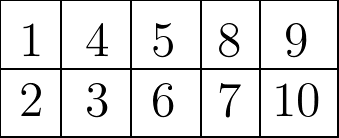
\includegraphics[width=0.3\textwidth]{pic02}}
\end{figure}

Женя прыгнула снаружи в~клетку~1, затем попрыгала по~остальным клеткам (каждый прыжок~--- на~соседнюю по~стороне клетку) и~выпрыгнула наружу из~клетки~10.
Известно, что на~клетке~1 Женя была один~раз, на~клетке~2~--- два~раза, \ldots, на~клетке~9~--- девять~раз.
Сколько раз побывала Женя на~клетке~10?

\item
Замок в~форме треугольника со~стороной 50 метров разбит на~100 треугольных залов со~сторонами $5\,\text{м}$.
В~каждой стенке между залами есть дверь.
Какое наибольшее число залов сможет обойти турист, не~заходя ни~в~какой зал дважды?

%\item а) На~шахматной доске стоят две одинаковых фишки.
%За~один ход можно сдвинуть одну из~фишек на~соседнее поле по~вертикали или горизонтали. Могут~ли фишки перейти в~симметричную относительно средней линии позицию ровно за~2015 ходов?\\
%б) На~шахматной доске стоят пять одинаковых фишек.
%За~один ход можно сдвинуть одну из~фишек на~соседнее поле по~вертикали или горизонтали. Могут~ли фишки перейти в~центрально симметричную позицию ровно за~2015 ходов?

\item а) Докажите, что следующий граф~--- двудольный:
Вершины графа~--- расстановка пары фишек на~шахматной доске. Две расстановки связаны ребром, если позиции0 получаются друг из~друга ходом фишки на~одну клетку по~вертикали или горизонтали.\\
б) На~шахматной доске стоят две одинаковых фишки.
За~один ход можно сдвинуть одну из~фишек на~соседнее поле по~вертикали или горизонтали. Так ходили, пока не~прошли через все возможные позиции. Докажите, что какая-то позиция встретилась не~менее двух раз.

%\item В клетки доски $8\times 8$ записали числа $1, 2,\dots, 64$ в неизвестном порядке. Разрешается узнать сумму чисел в любой паре клеток с общей стороной. Всегда ли можно узнать расположение всех чисел? 
\item а) 10 кружковцев образовали дежурную команду для решения домашних задач. В команде всегда не менее 3 человек. Каждый вечер в команду добавляется один человек либо из неё исключается один человек. Можно ли будет перебрать все допустимые составы команды ровно по одному разу?\\
б) Возможно ли это при другом первоначальном количестве кружковцев?

\item На клетчатой доске $11\times 11$ отмечено 22 клетки так, что на каждой вертикали и на каждой горизонтали отмечено ровно 2 клетки. Два расположения отмеченных клеток эквивалентны, если, меняя любое число раз вертикали между собой и горизонтали между собой, мы из одного расположения можем получить другое. Сколько существует неэквивалентных расположений отмеченных клеток?
\end{problems}

\resetproblem
\vspace{1cm}
\addcontentsline{toc}{abcd}{\bf Площади. 7 июля}
\begin{center}
\textbf{\Large Площади}\\
%\textit{Профи}\\
\textit{07.07.16}

\epigraph{\it Я никогда не читаю, я просто смотрю на картинки.}{Энди Уорхол}

\definition Каждой фигуре $M$ на плоскости ставится в соответствие число $S_M$, называемое \textit{площадью}, такое, что выполнены следующие свойства:

\begin{enumerate}
	\item $S_M > 0$;
	\item Площади равных фигур равны;
	\item Если фигура $M$ состоит из фигур $A$ и $B$, не имеющих общих точек, то $S_M = S_A + S_B$;
\end{enumerate}

\end{center}

\begin{problems}

\item (\textit{Рельсы Евклида})
Дан прямоугольник $ABCD$. \\
а) На $BC$ взята точка $K$. Докажите, что $S_{ABCD} = 2 S_{AKD}$.\\
б) На $BC$ взяты точки $K$ и $L$. Докажите, что $S_{AKD} = S_{ALD}$. \\
в) Будут ли верны эти результаты, если точки $K$ и $L$ взять на прямой $BC$? \\ 
\item
Докажите, что закрашенные параллелограммы равны по площади.
%1.jpg

\item
Докажите, что закрашена половина площади параллелограмма (точка~--- произвольная внутренняя точка параллелограмма). 
%2b.jpg

\item (\textit{Лемма о линолеуме}) Если пол в комнате площадью $S$ надо покрыть линолеумом общей площадью также $S$ так, чтобы не было участков, покрытых более чем в два слоя, то площадь пола, покрытая дважды, равна площади пола, не покрытой ни разу. Докажите лемму.


\item
Докажите, что сумма площадей незакрашенных фигур равна сумме площадей фигур, закрашенных тёмным.
%2c.jpg, 2d.jpg


\item
Докажите, что а) медиана треугольника делит его на два треугольника равной площади;\\
б) пусть чевиана (то есть отрезок, соединяющий вершину треугольника с точкой на противолежащей стороне) делит сторону в отношении $m:n$. Тогда площади получившихся треугольников относятся как $m:n$. 

\item
Выразите $X$ через $S$ ($X = S_{ABC}$). \\
\item
В пятиугольнике $ABCDE$ стороны $BC$ и $CD$ параллельны соотвественно диагоналям $AD$ и $BE$. Докажите, что треугольники $ABC$ и $CDE$ равновелики.
%12

\item
Через точку $D$, лежащую на стороне $BC$ треугольника $ABC$, проведены прямые параллельные двум другим сторонам и пересекающие стороны $AB$ и $AC$ соответственно в точках $E$ и $F$. Докажите, что треугольники $CDE$ и $BDF$ равновелики.

\item
Внутри параллелограмма $ABCD$ взяли произвольную точку $M$. Прямая $BM$ пересекает $AD$ в точке $E$. Докажите что площади треугольников $AMD$ и $CME$ равны.
%23

%\item
%В пятиугольнике $ABCDE$ стороны $AB,BC$ И $CD$ параллельны диагоналям $CE, AD$ и $BE$ соответственно. Верно ли, что треугольники $ABE$ и $CDE$ равновелики?
%13

\item (\textit{Теорема Пифагора})
Докажите, что сумма площадей квадратов построенных на катетах, равна площади квадрата построенного на гипотенузе, используя рельсы Евклида.

\item В параллелограмме $ABCD$ проведены четыре отрезка~--- вершина $A$ соединена с серединой стороны $BC$, вершина~--- $B$ с серединой стороны $CD$, вершины $C$ и $D$~--- с серединами сторон $AD$ и $AB$ (соответственно). Докажите, что четырехугольник, образуемый этими четырьмя отрезками~--- параллелограмм, и что его площадь в пять раз меньше площади данного параллелограмма.
\end{problems}

\begin{figure}[!h]
\minipage{.32\textwidth}
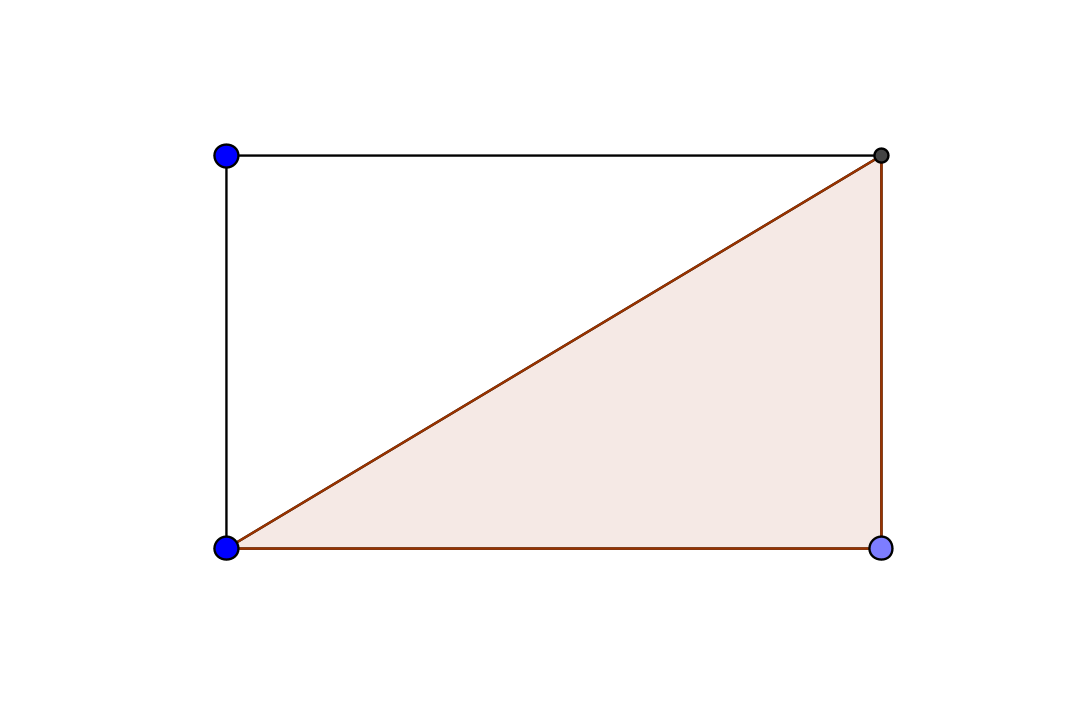
\includegraphics[width=1.2\linewidth]{0a}
\caption{1a)}
\endminipage\hfill
\minipage{.32\textwidth}
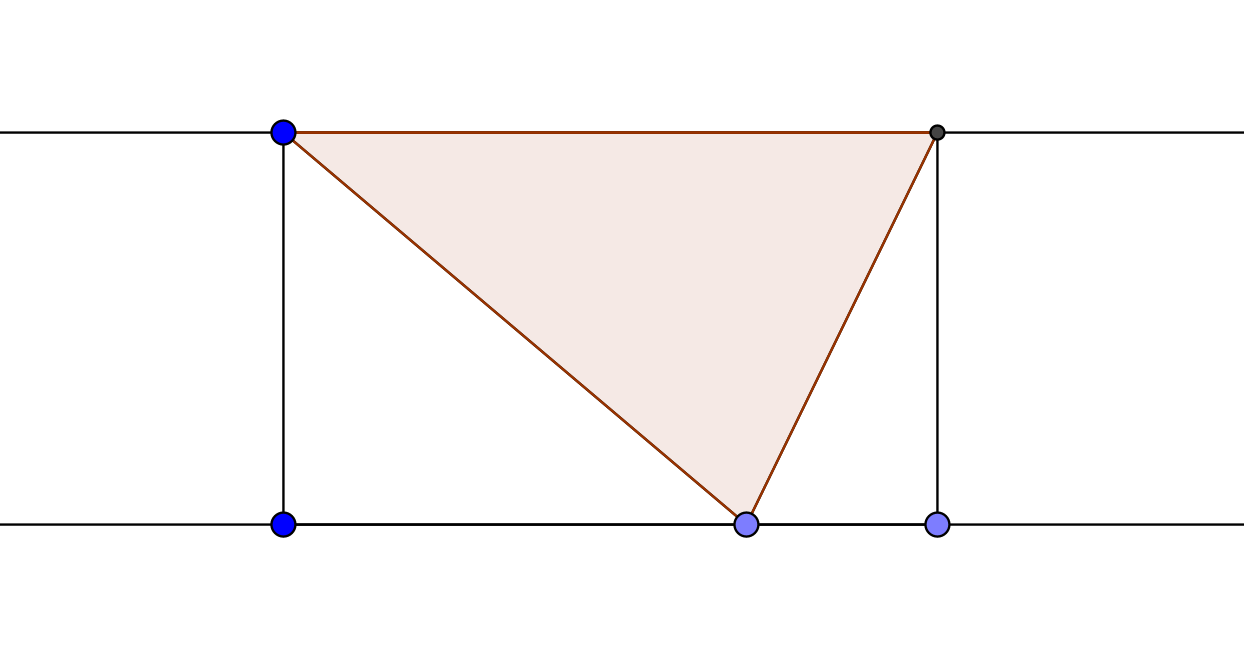
\includegraphics[width=1.2\linewidth]{0c}
\caption{1a)}
\endminipage\hfill
\minipage{.32\textwidth}
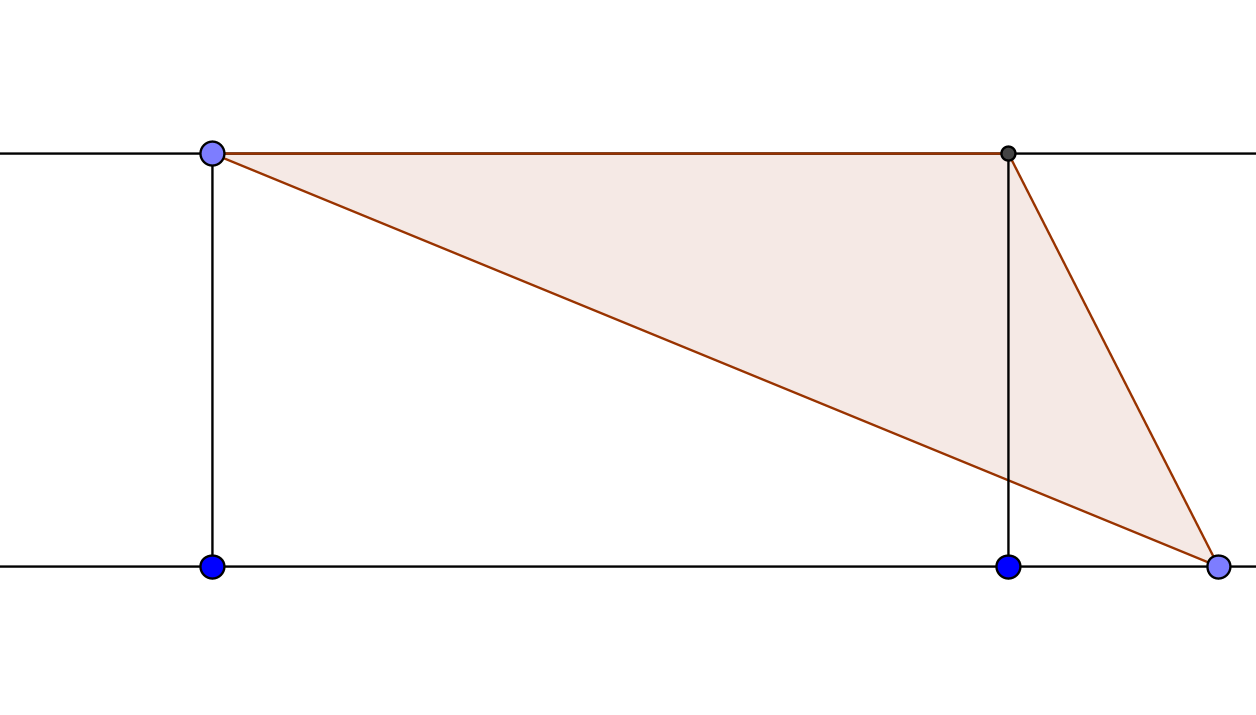
\includegraphics[width=1.2\linewidth]{0b}
\caption{1c)}
\endminipage
\end{figure}

\begin{figure}[!h]
\minipage{.32\textwidth}
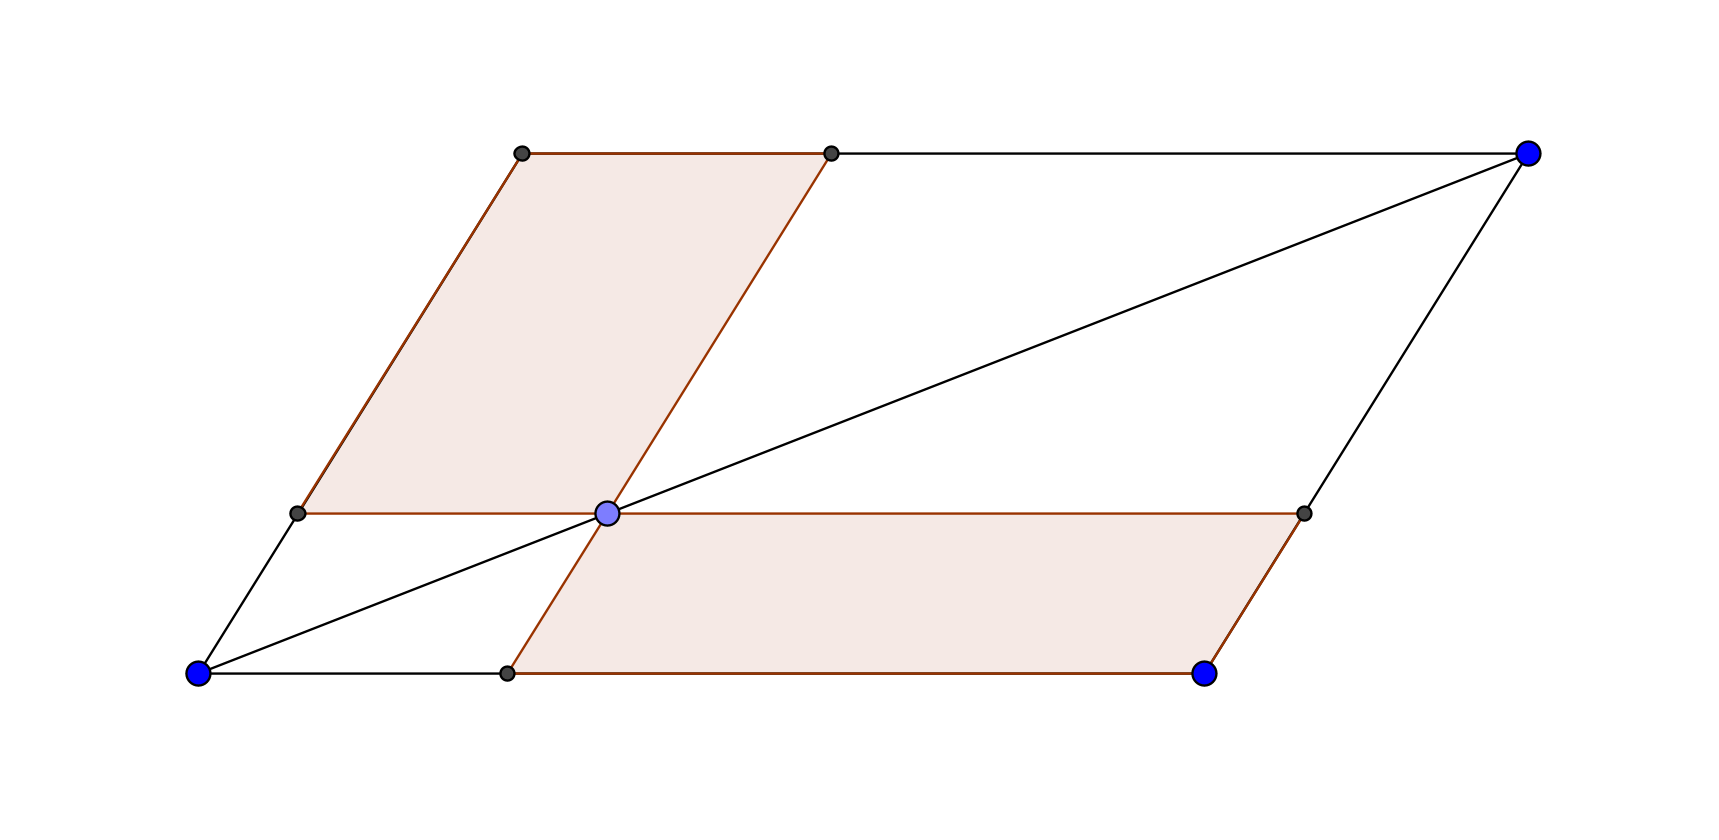
\includegraphics[width=1.2\linewidth]{1}
\caption{2)}
\endminipage\hfill
\minipage{.32\textwidth}
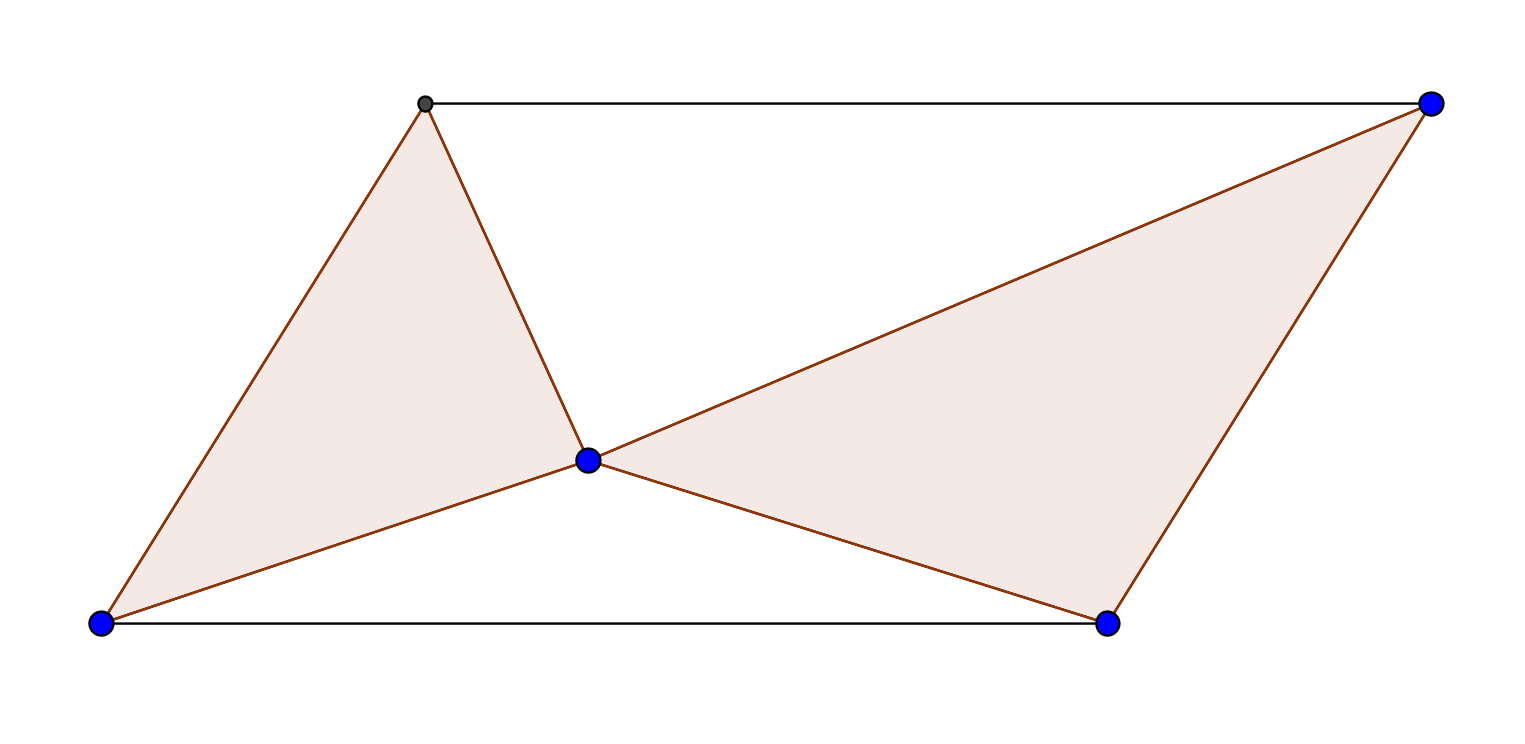
\includegraphics[width=1.2\linewidth]{2b}
\caption{3)}
\endminipage\hfill
\minipage{.32\textwidth}
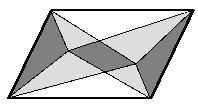
\includegraphics[width=1.2\linewidth]{2d}
\caption{5a)}
\endminipage
\end{figure}

\begin{figure}[!h]
\minipage{.32\textwidth}
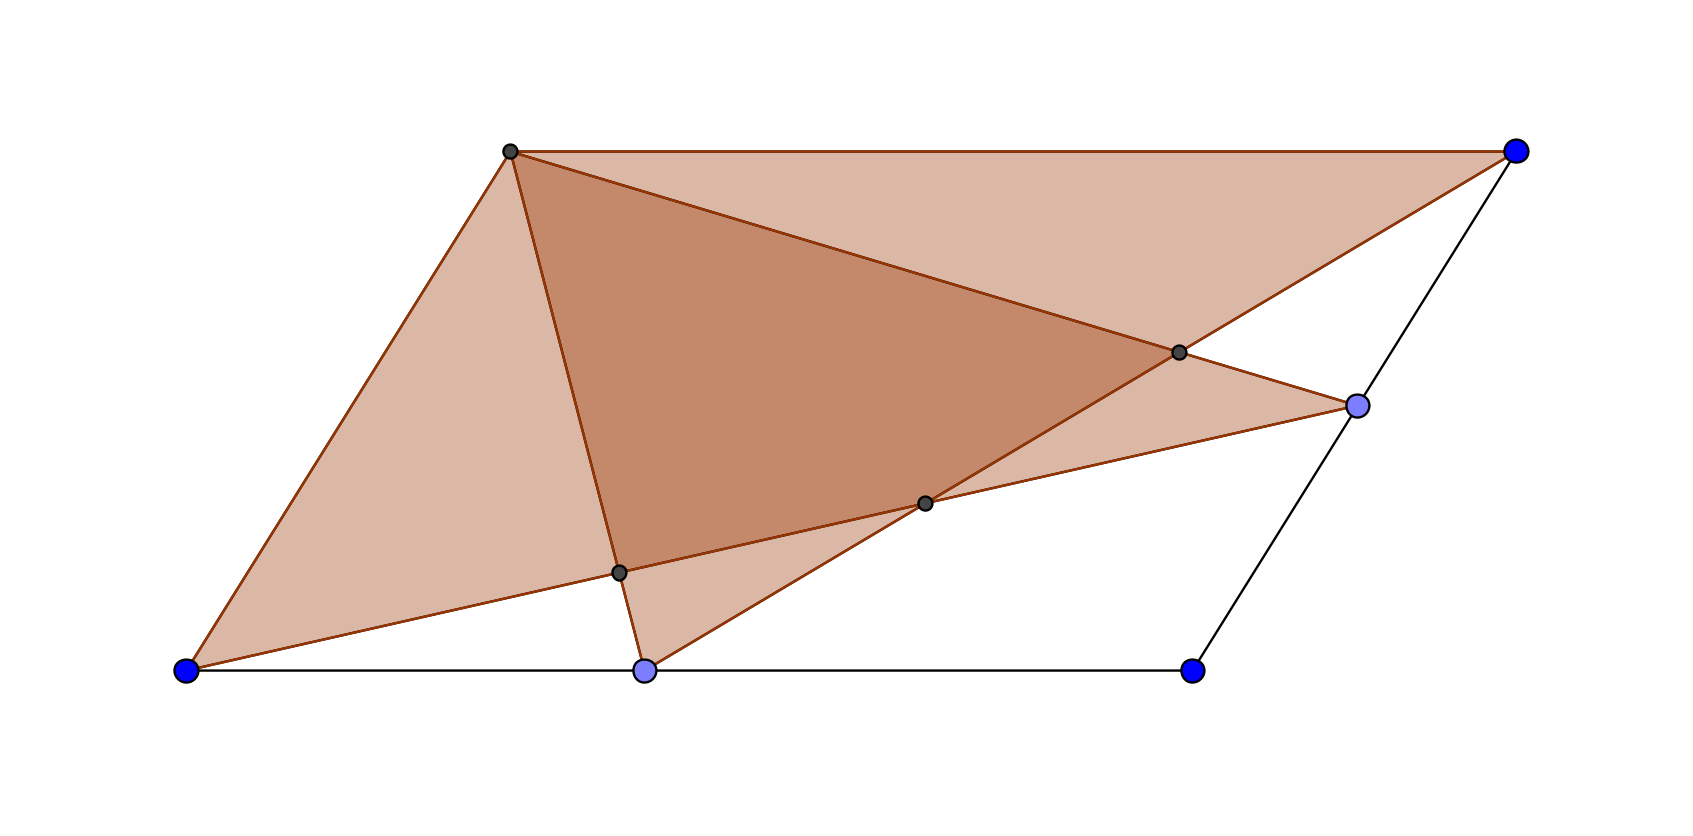
\includegraphics[width=1.2\linewidth]{2c}
\caption{5b)}
\endminipage\hfill
\minipage{.32\textwidth}
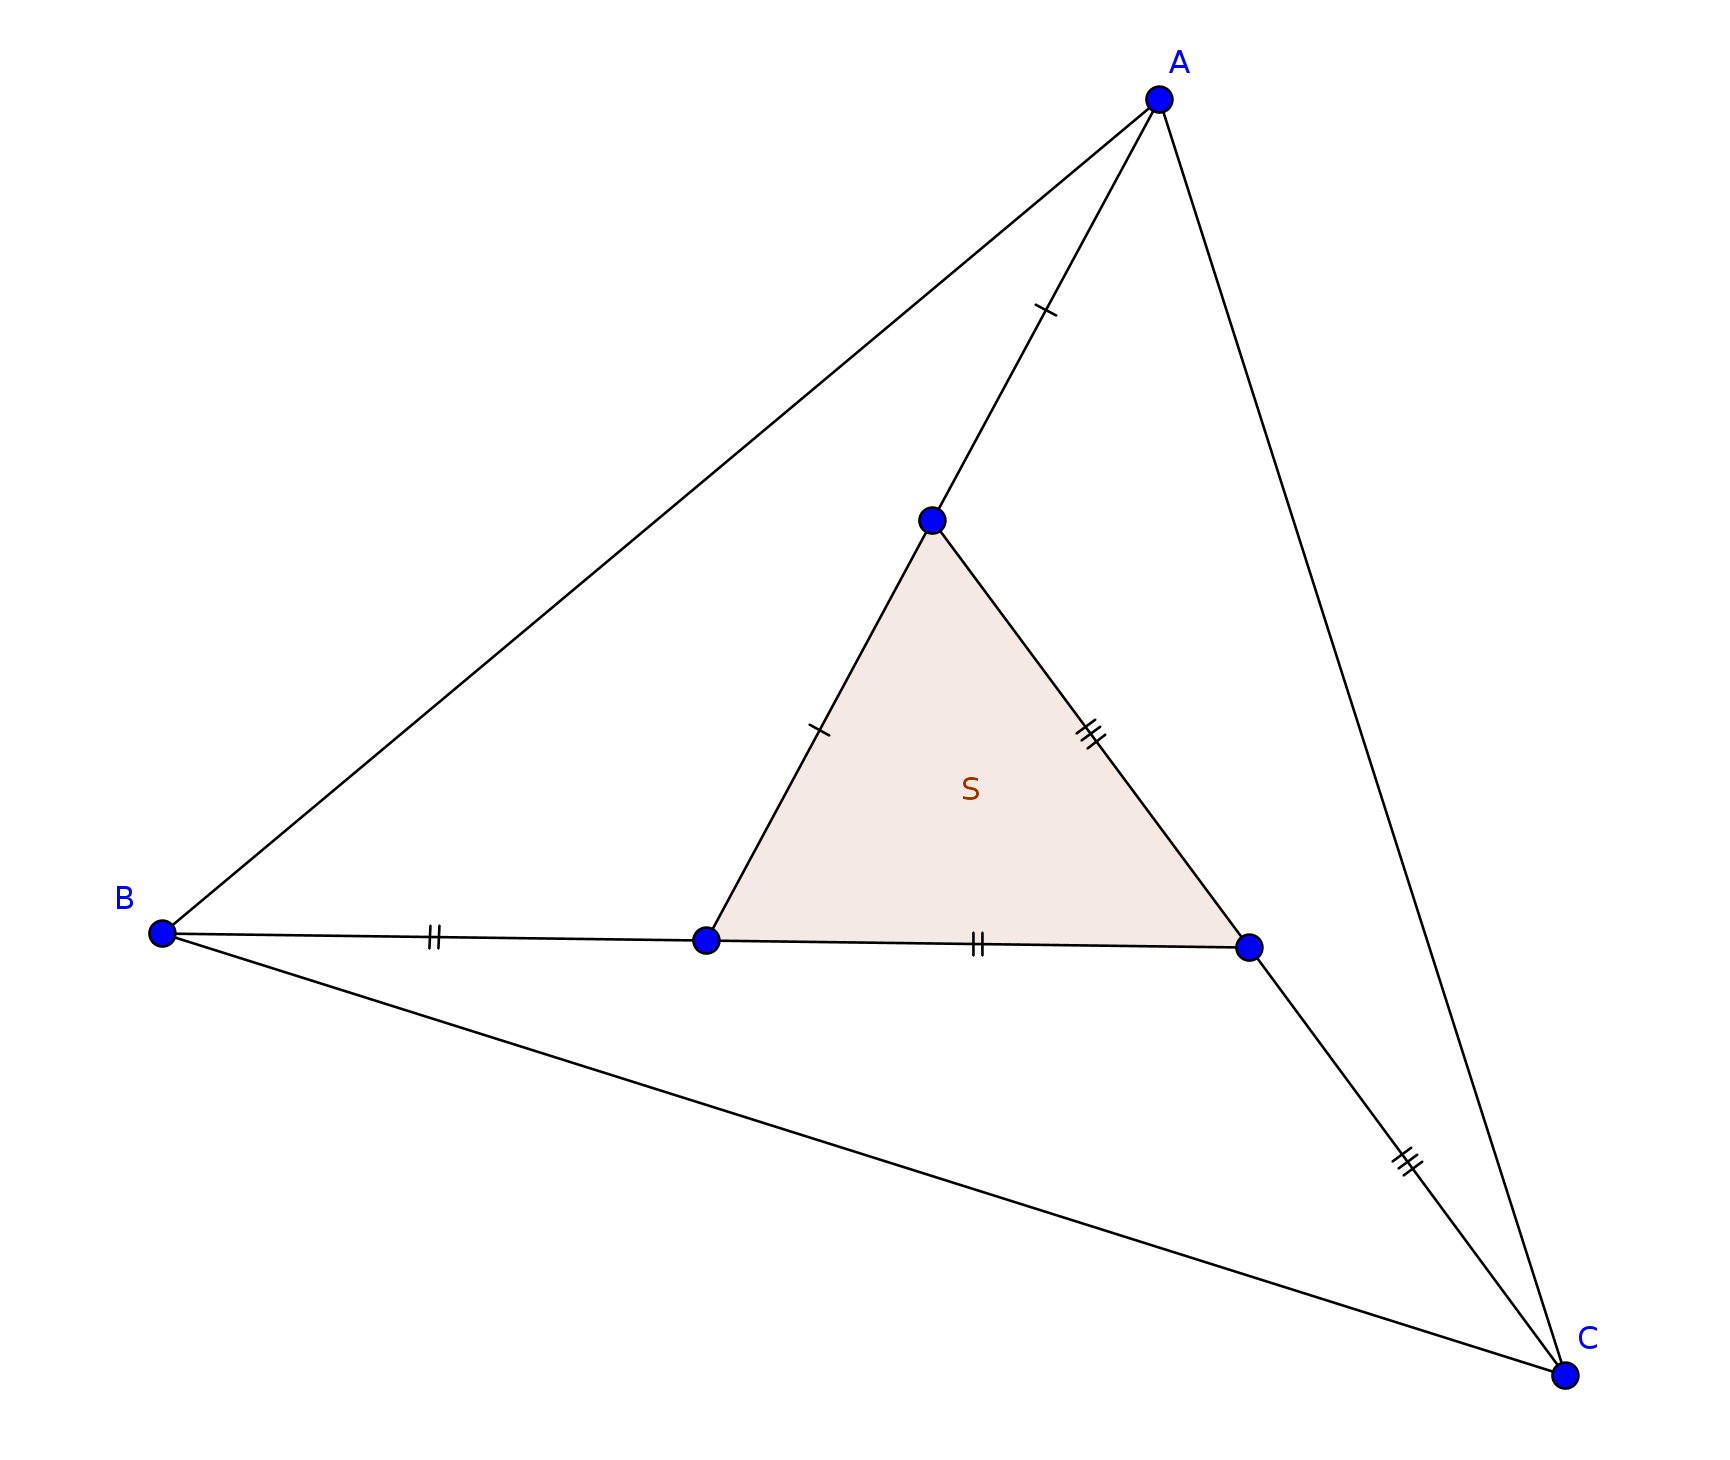
\includegraphics[width=1.2\linewidth]{7a}
\caption{7a)}
\endminipage\hfill
\minipage{.32\textwidth}
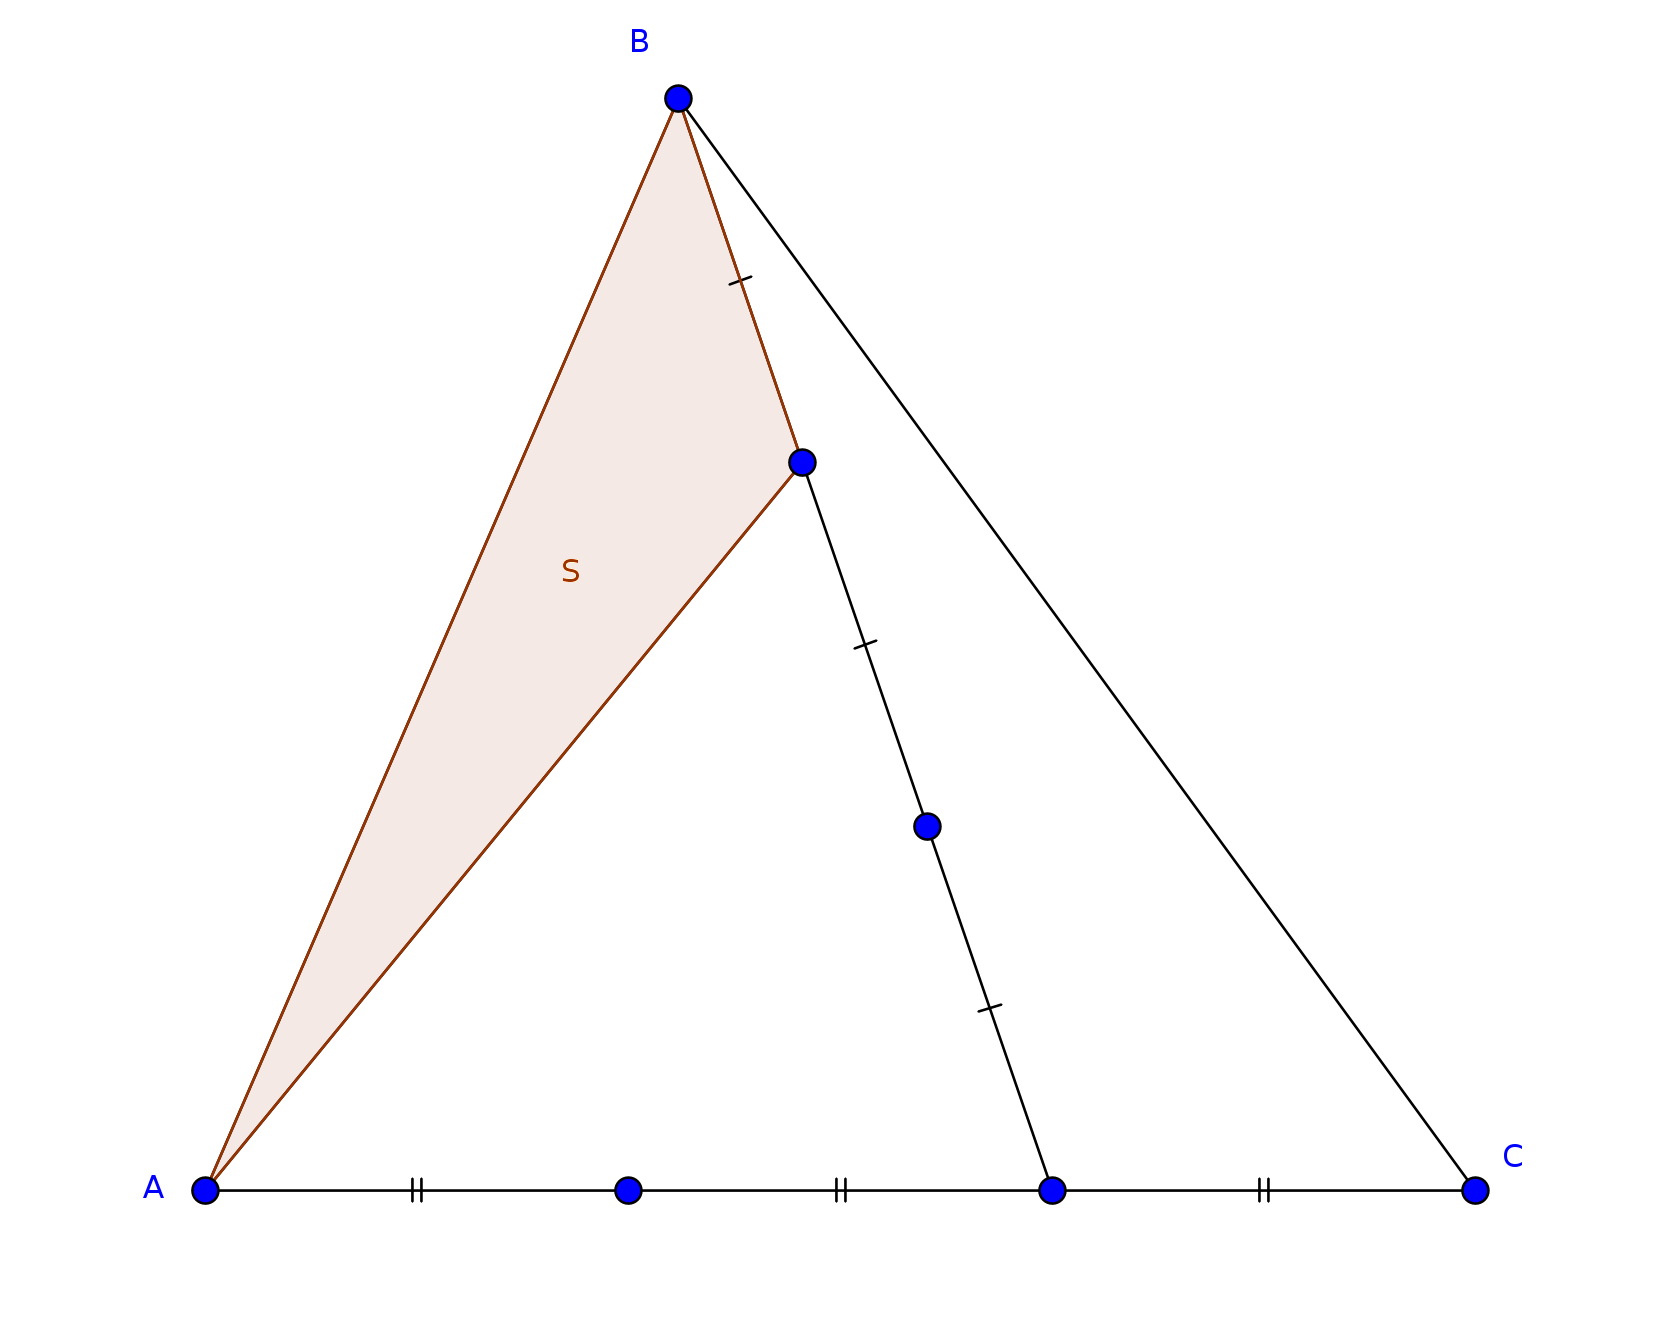
\includegraphics[width=1.2\linewidth]{7b}
\caption{7b)}
\endminipage
\end{figure}

\begin{figure}[!h]
\minipage{.32\textwidth}
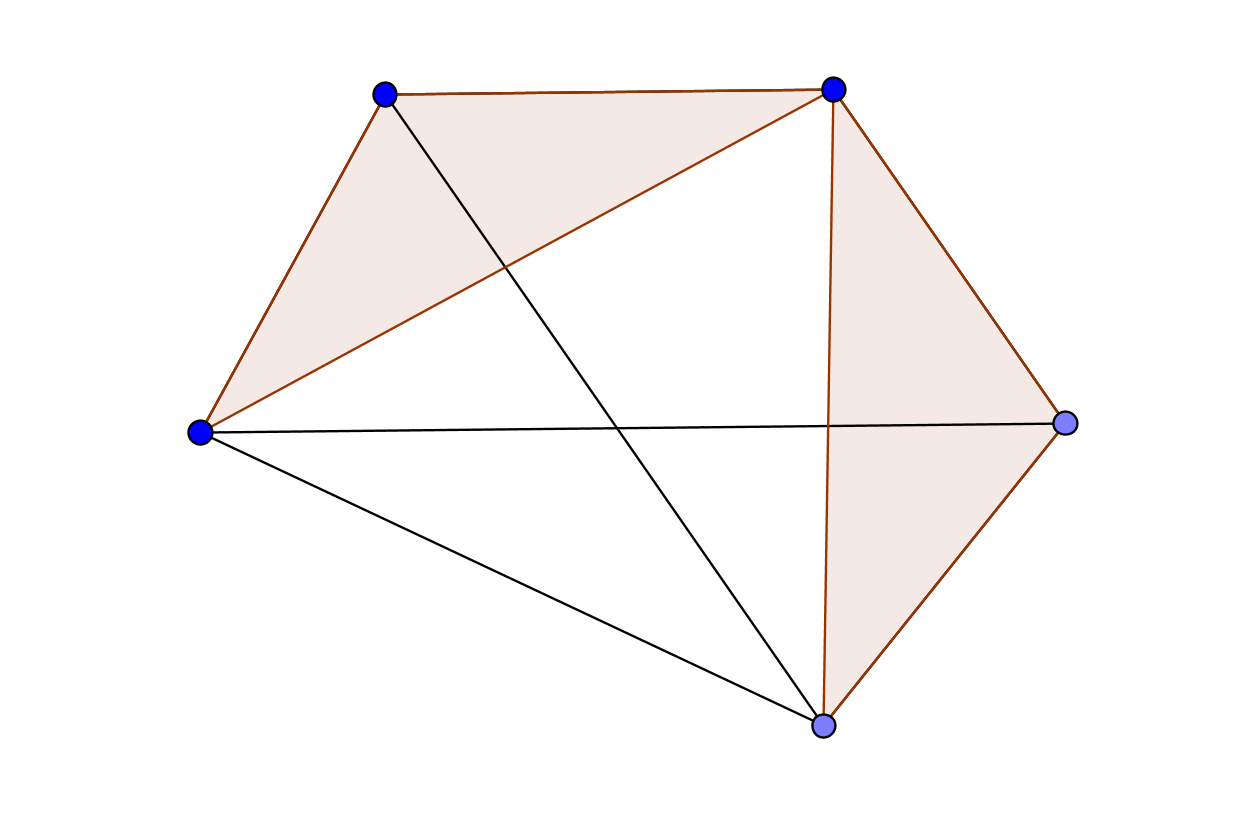
\includegraphics[width=1.2\linewidth]{5}
\caption{8)}
\endminipage\hfill
\minipage{.32\textwidth}
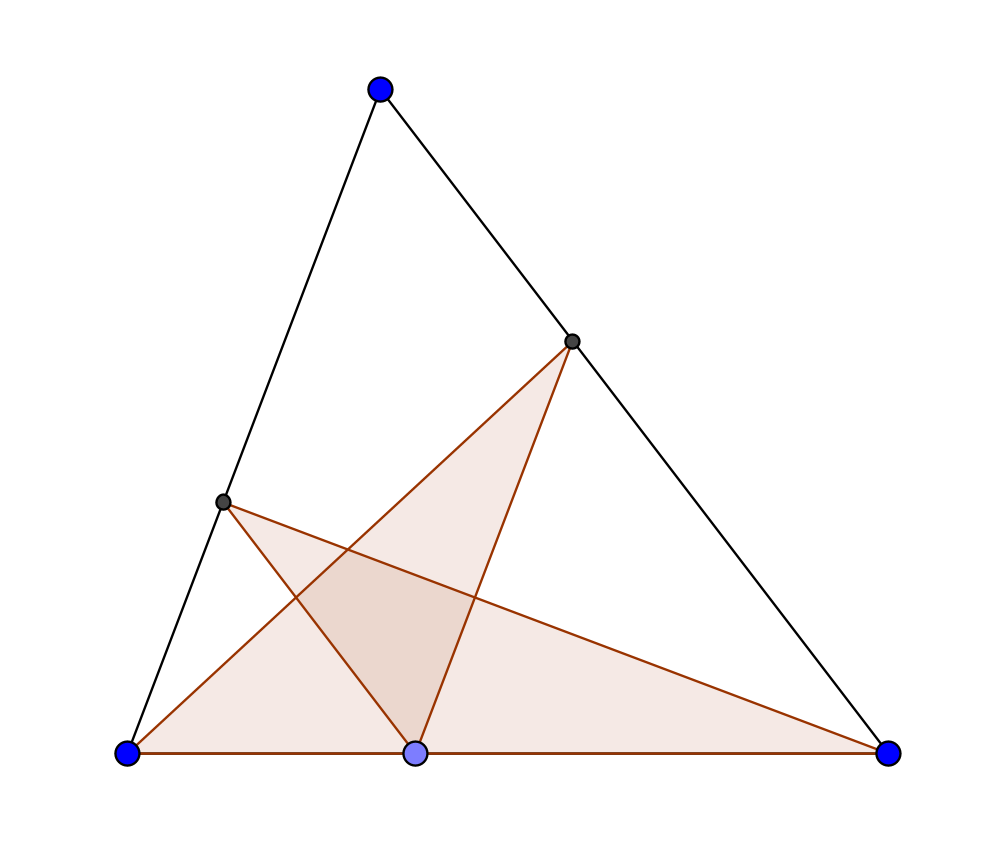
\includegraphics[width=1.2\linewidth]{6}
\caption{9)}
\endminipage\hfill
\minipage{.32\textwidth}
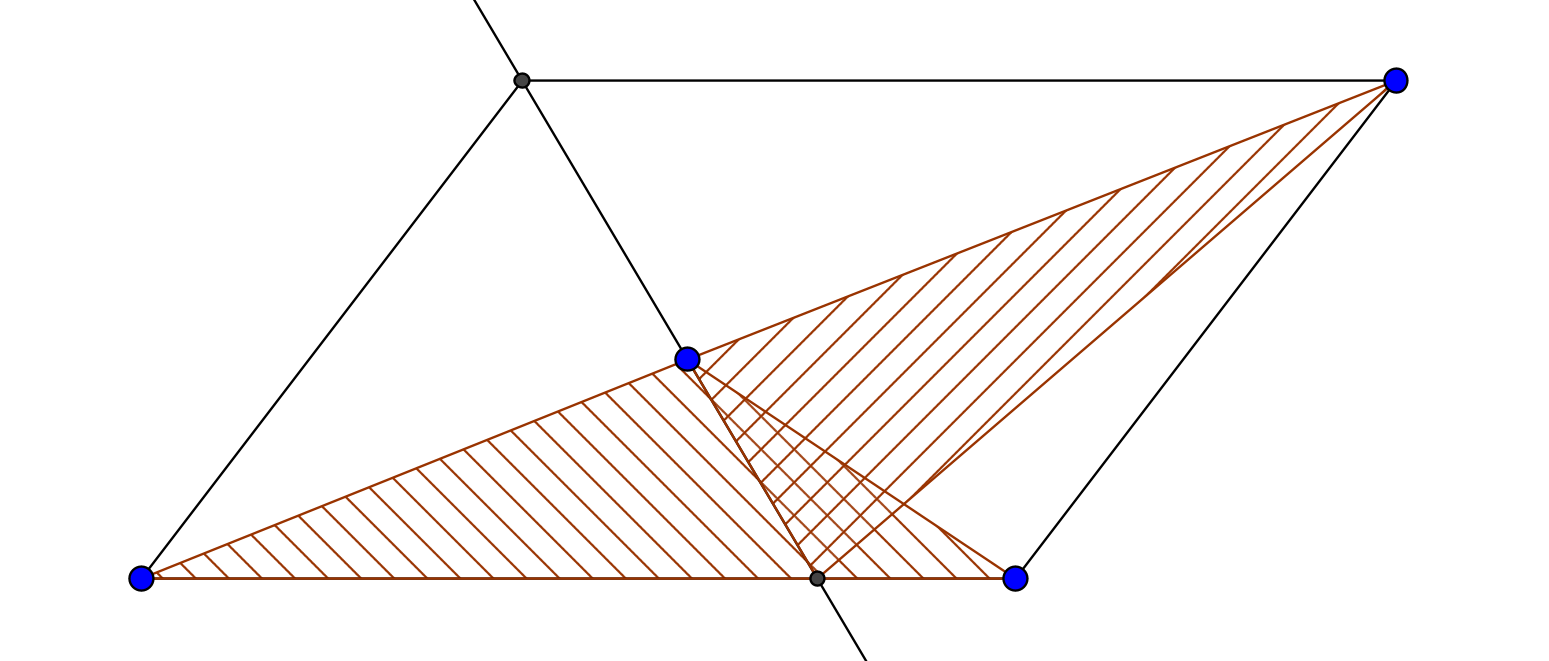
\includegraphics[width=1.2\linewidth]{3}
\caption{10)}
\endminipage
\end{figure}

\begin{figure}[!h]
\minipage{.32\textwidth}
% \includegraphics[width=\linewidth]{5d}
% \caption{7)}
\endminipage\hfill
\minipage{.32\textwidth}
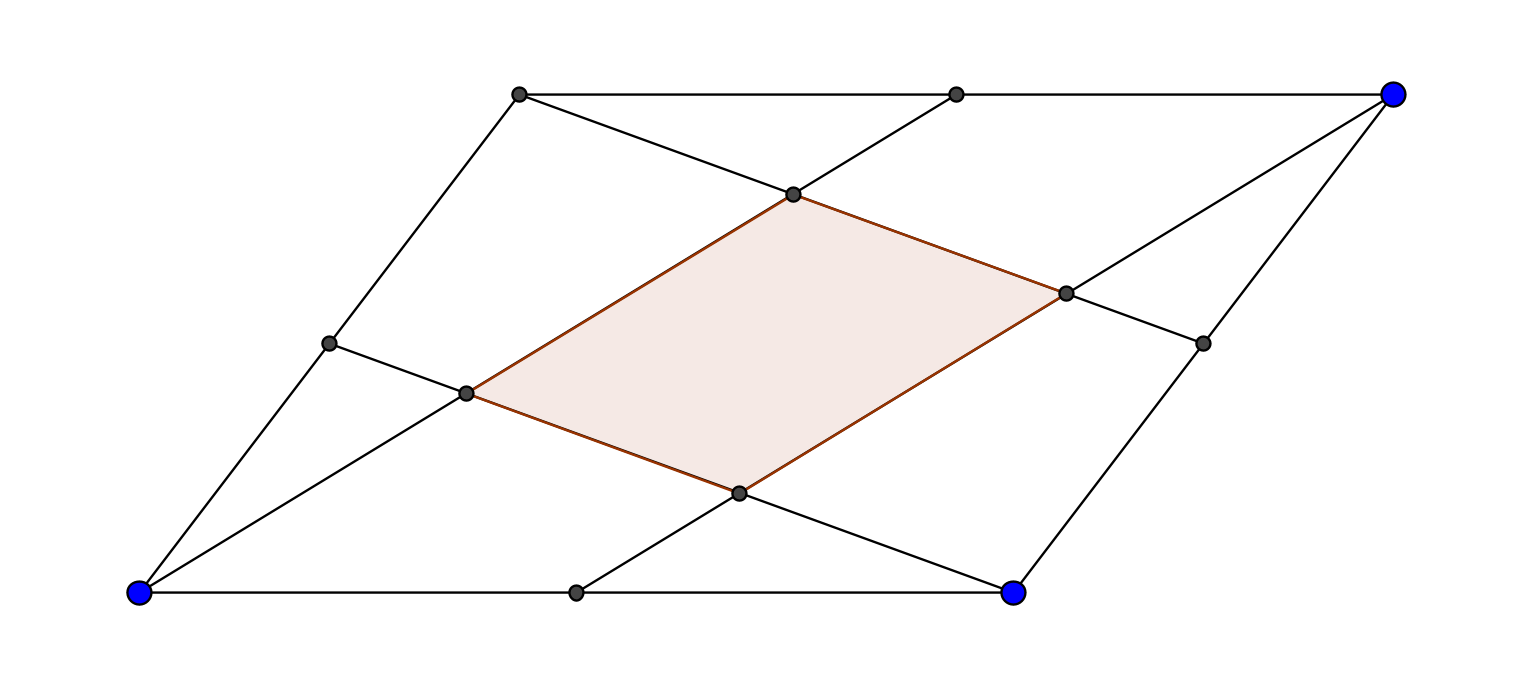
\includegraphics[width=1.2\linewidth]{4}
\caption{12)}
\endminipage\hfill
\minipage{.32\textwidth}
% 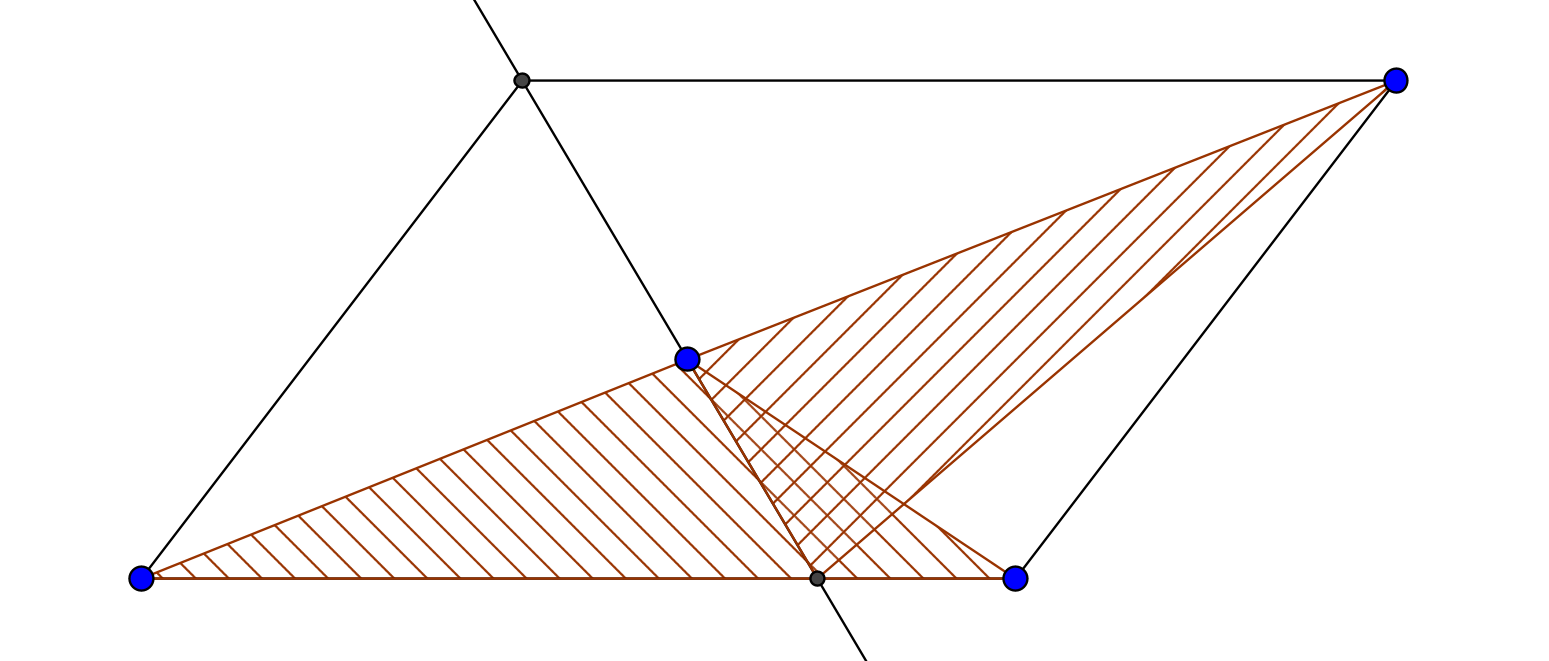
\includegraphics[width=\linewidth]{3}
% \caption{10)}
\endminipage
\end{figure}

\resetproblem
\vspace{1cm}
\addcontentsline{toc}{abcd}{\bf Классическая комбинаторика. 7 июля}
\begin{center}
\textbf{\Large Классическая комбинаторика}\\
%\textit{Профи}\\
\textit{07.07.16}
\end{center}

\epigraph{\it Это знать надо! Это классика!}{Товарищ капитан}

\textit{Материалы для работы по группам на второй паре. Цель работы~--- доказать следующие равенства комбинаторно. У разных групп разные наборы неравенств.}

\begin{problems}
\item $kC_n^k=nC_{n-1}^{k-1}$

\item $C_n^0\cdot 2^0+C_n^1\cdot 2^1+\cdots+C_n^n\cdot 2^n=3^n$

\item $C_n^0 C_n^m + C_n^1 C_{n-1}^{m-1} + \cdots + C_n^m C_{n-m}^{n-m}=2^m C_n^m$

\item $C_k^k+C_{k+1}^k+\cdots+C_n^k=C_{n+1}^{k+1}$

\item $C^1_n + 6C^2_n + 6C^3_n = n^3$
\end{problems}
\resetproblem
\vspace{5pt}
\hrule
\begin{problems}
\item $C_n^{k-1}+C_n^{k}=C_{n+1}^k$

\item $C_p^0 C_q^k + C_p^1 C_q^{k-1}+\cdots +C_p^{k-1} C_q^1 ++C_p^k C_q^0=C_{p+q}^k$

\item $0\cdot C_n^0 + 1\cdot C_n^1 + 2\cdot C_n^2+\cdots+n\cdot C_n^n=n\cdot 2^{n-1}$

\item $C_{n-1}^0+C_n^1+C_{n+1}^2+\cdots+C_{n+m-1}^m=C_{n+m}^m$

\item $1 + 14C^1_n + 36C^2_n + 24C^3_n = (n + 1)^4 - n^4$
\end{problems}
\resetproblem
\vspace{5pt}
\hrule
\begin{problems}
\item $C_r^m C_m^k=C_r^k C_{r-k}^{m-k}$

\item $C_n^0+C_n^2+C_n^4+\dots=C_n^1+C_n^3+C_n^5+\dots=C_{n-1}^0+C_{n-1}^1+\cdots+C_{n-1}^{n-1}$

\item $(C_n^0)^2 + (C_n^{1})^2+\cdots+(C_n^n)^2=C_{2n}^n$

\item $C_{n-1}^0+C_n^1+C_{n+1}^2+\cdots+C_{n+m-1}^m=C_{n+m}^m$

\item $C^1_n + 14C^2_n + 36C^3_n + 24C^4_n = n^4$
\end{problems}
\resetproblem
\vspace{5pt}
\hrule

\begin{problems}
\item Сколькими способами могут выпасть три различные игральные кости?

a. Во скольких случаях хотя бы на одной кости будет 6 очков?

b. Ровно на одной будет 6 очков?

c. Ровно на одной 6, а ровно на одной другой 3 очка?

\item Имеется $n$ абонентов телефонной сети. Сколькими способами можно одновременно соединить 3 пары абонентов?

\item Сколькими способами можно выстроить в шеренгу 5 футболистов, 5 бегунов и 5 боксёров так, чтобы никакие два боксёра не стояли рядом (отличить двух спортсменов, занимающихся одним видом спорта, невозможно).

\item В выпуклом $n$-угольнике никакие три диагонали не пересекаются в одной
точке. Найдите количество точек пересечения диагоналей.

\item Пусть $p>2$~--- простое число. Сколько существует способов раскрасить вершины правильного $p$-угольника в $a$ цветов? (раскраски, которые можно совместить поворотом, считаются одинаковыми.) 

\item Пусть $p>2$~--- простое число. Сколькими способами можно провести через вершины правильного $p$-угольника замкнутую ориентированную $p$-звенную ломаную? (ломаные, которые можно совместить поворотом, считаются одинаковыми.) 

\end{problems}

\resetproblem
\vspace{1cm}
\addcontentsline{toc}{abcd}{\bf ГМТ. 9 июля}
\begin{center}
\textbf{\Large ГМТ}\\
%\textit{Профи}\\
\textit{09.07.16}
\end{center}

\epigraph{\it В общем случае, геометрическое место точек формулируется параметрическим предикатом, аргументом которого является точка данного линейного пространства.}{Википедия}

\textbf{Обозначение.} {\itГеометрическим местом точек (ГМТ)} называется фигура, состоящая из все точек плоскости, которые удовлетворяют какому-либо определенному условию.

%примеры: окружность, круг



\begin{problems}

\item   a) Найдите ГМТ, равноудаленных от точек $A$ и $B$;\\
b) Найдите ГМТ, равноудаленных от двух заданных прямых;\\
c) Найдите ГМТ, равноудаленных от сторон заданного угла;\\
d) Дан отрезок $AB$. Найдите ГМТ таких, что $AM<BM$.

%\item   Дан четырехугольник $ABCD$. Где находится такая точка $O$, что $AO=CO$ и $BO=DO$? Сколько может быть таких точек?

\item  Дан четырехугольник $ABCD$. Оказалось, что существуют две такие точки $O$, что $AO=DO$ и $BO=CO$. Докажите, что $AD$ и $BC$ параллельны.

\item  Дан отрезок $AB$.  Найдите ГМТ $M$ таких, что $AM$ --- наименьшая сторона треугольника $ABM$ (ответ дайте в виде заштрихованной области).

\item   Даны точки $A$ и $B$. Найдите ГМТ $M$ таких, что угол $ \angle BAM< \angle AMB < \angle ABM$.

%\item  Дан треугольник $ABC$. Некоторая точка $M$ такова, что $AM=1$, $BM=2$, $ CM=3$. Единственна ли такая точка $M$?

\item   На прямой выбран отрезок $AB$. Из точки $D$ на этой прямой, но вне отрезка, восстановлен перпендикуляр $CD$ такой, что $AB=CD$. Сколько существует точек $M$ таких, что треугольники $ABM$ и $CDM$ равны?

%\item  Точка $O$ --- середина отрезка $MK$. Известно, что $AM<BM$,  $AK<BK$. Докажите, что $AO<BO$.

\item   Диагонали четырехугольника равны. Известно, что серединный перпендикуляр к одной его стороне пересекает противоположную сторону. Докажите, что это верно и для противоположной стороны.

\item   Дан шестиугольник, никакие стороны которого не параллельны. Стороны покрашены в черный и белый цвет по очереди. Сколько существует точек, которые равноудалены от всех черных сторон?

%\item  В четырехугольнике $ABCD$ внешний угол при вершине $A$ равен углу $BCD$, $AD=CD$. Докажите, что $BD$ --- биссектриса угла $ABC$.

%\item   Дан квадрат $ABCD$. Найдите ГМТ, сумма расстояний от которых до прямых $AB$ и $CD$ равна сумме расстояний до прямых $AD$ и $BC$.

\item   Пусть $O$ --- центр правильного треугольника $ABC$. Найдите ГМТ $M$, удовлетворяющих следующему условию: любая прямая, проведенная через точку $M$, пересекает либо отрезок $AB$, либо отрезок $CO$.

%\item   Даны прямая $l$ и точки $A$ и $B$ по одну сторону от нее. Найдите ГМТ $M$ таких, что прямая $AM$ пересекает прямую $l$ левее, чем прямая $BM$.

% с выходом на среднюю линию
\item На сторонах $AB$ и $BC$ треугольника $ABC$ берутся точки $D$ и $E$ (по одной на каждой). Найдите геометрическое место середин отрезков $DE$.

% знаю только сложное решение с окружностями, а должно быть и доброе
\item Найдите геометрическое место точек $M$, лежащих внутри ромба $ABCD$ и обладающих тем свойством, что  $ \angle AMD +  \angle BMC = 180^\circ$.


\end{problems}

\resetproblem
\vspace{1cm}
\addcontentsline{toc}{abcd}{\bf Индукция. 9 июля}
\begin{center}
\textbf{\Large Индукция}\\
%\textit{Профи}\\
\textit{09.07.16}
\end{center}

\epigraph{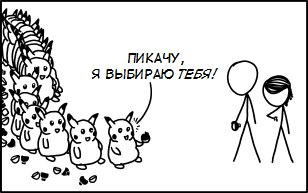
\includegraphics[width=.8\textwidth]{ind.jpg}}{http://xkcd.ru/1516/}

\begin{problems}
\item Из квадрата $2^n \times 2^n$ вырезали одну клетку. Докажите,
что полученную фигуру можно разрезать на уголки из трёх клеток.

\item
На сколько частей делят плоскость $n$ прямых, среди которых нет
параллельных, и никакие три не пересекаются в одной точке?

\item
Докажите, что $1 + 2 + 3 + \ldots + n = \dfrac{n(n+1)}{2}$.

\end{problems}

\resetproblem

%\q4.
%ханойские башни

%\q5.
%Докажите, что $3^{2n+2}+8n-9$ делится на 16.

%\q6.
%{\itshape Утверждение.} У всех людей глаза одинакового цвета. \\
%{\itshape Доказательство. } Докажем, что в компании из $n$  людей у всех глаза одинакового цвета, методом
%математической индукции.
%При     $n=1$    утверждение очевидно. \\

%Предположим, что в любой компании из $k$  человек у всех глаза одинакового цвета. Рассмотрим
%компанию из   $k+1$   человека. Перенумеруем их: первый, второй, третий, …, $k$ -ый,    $(k+1)$ -ый. По
%предположению, у любых   из этих людей глаза одинакового цвета. Значит, у первого, второго,
%…,  $k$-го — глаза одинакового цвета. \\

%Возьмём теперь другую группу из человек: второй, третий, …,  $k$-ый, $(k+1)$-ый. У них тоже
%глаза одинакового цвета. В обеих группах присутствовал второй человек. Значит у всех них глаза
%того же цвета, как и у второго, то есть у всех одинаковые. {\bf Где же ошибка?}


{\bf Задачи для самостоятельного решения.}


\begin{problems}
%равенства
\item
Докажите, что $1^2 + 2^2 + \ldots + n^2 = \dfrac{n(n+1)(2n+1)}{6}.$

%\item
%Докажите, что $1^3+2^3+3^3+ \ldots + n^3 = %\dfrac{n^2(n+1)^2}{4}$

\item
Докажите, что $1 \cdot 1! + 2 \cdot 2! + \ldots + n \cdot n! = (n+1)! - 1.$

%\item
%Докажите, что для любого $x \ne 1$ $1 + x + x^2 + %\ldots + x^n =
%\frac{x^{n+1} - 1}{x - 1}$

\item
Докажите, что $\frac{1}{1 \cdot 2} + \frac{1}{2 \cdot 3} + \ldots + \frac{1}{n \cdot (n+1)} = 1 - \frac{1}{n+1}.$

%\item
%Докажите равенство $3 + 33 + 333 + \ldots + \underbrace{33 \ldots
%33}_n = \dfrac{10^{n+1} - 9n - 10}{27}$

%\item
%Докажите, что
%$$ (1 - \frac{1}{4}) (1 - \frac{1}{9}) \ldots (1 - \frac{1}{n^2}) = \frac{n+1}{2n}$$

%полегче

\item
У бородатого многоугольника во внешнюю сторону растет щетина. Его
пересекает несколько прямых, на каждой из которых с одной из сторон
тоже растет щетина. В результате многоугольник оказался разбитым на
некоторое число частей. Докажите, что хотя бы одна из частей
окажется бородатой снаружи (никакие три прямые не проходят через
одну точку).

\item
Плоскость поделена на области несколькими прямыми. Докажите, что эти
области можно раскрасить в два цвета так, чтобы любые две соседние
области были раскрашены в различные цвета.



%средние



\item
Докажите, что если клетчатая доска $n \times n$ покрашена в 4 цвета
так, что любой квадрат $2 \times 2$ содержит все четыре цвета, то:
если $n$~--- чётно, то в углах квадрата стоят разные цвета; если $n$~---
нечётно, то клетки в углах раскрашены не более, чем в 2 цвета.

%\item
%Кусок бумаги разрешается рвать на 4 или на 6 кусков. Докажите, что по этим правилам его можно разорвать на любое число кусков, начиная с шести.

%\item Докажите, что любой квадрат можно разрезать на $n$ квадратов, начиная с шести.


\item
Пусть $x$~--- такое, что $x+ \frac{1}{x}$~--- целое. Докажите, что
$x^n + \frac{1}{x^n}$~--- целое для любого натурального $n$.

%сложные



\item
Доказать, что для любого натурального $n$ существует $n$-значное число, составленное из цифр $1$ и $2$, которое делится на $2^n$.

\item
В выпуклом многоугольнике некоторые стороны и диагонали окрашены в
красный цвет так, что никакие две красные диагонали не пересекаются
внутри многоугольника, а любые две вершины многоугольника соединены
ломаной из красных отрезков. Докажите, что сумма длин всех красных
отрезков больше полупериметра многоугольника.

\item 
Есть два квадрата со стороной $25\cdot 2^n$. В одном Василий Иванович отмечает одну клетку. Петька должен разрезать свой квадрат на части так, что:

(a) среди них есть квадратик со стороной $1$;

(b) какую бы клетку Василий Иванович не отметил бы, Петька сможет закрыть своими фигурками все клетки квадрата Чапаева, кроме отмеченной. 

Докажите, что Петьке достаточно разбить квадрат на $6+n$ деталей.



%\item
%Пусть $p$ -- простое и $gcd(n,p) = 1$. Докажите, что $n^{p-1}$ даёт остаток 1 при делении на $p$.

%\item На сколько частей делят пространство $n$ плоскостей,если никакие три из которых не пересекаются по одной прямой и никакие 4 из них не имеют общей точки? (на какое наибольшее число частей могут разбивать плоскость $n$ окружностей)

%\item есть жесть

%делимость

%\item Докажите, что $5 \cdot 2^{3n+1} + 3^{3n+2}$ делится на 19.

%\item Числа вида $F_n = 2^{2^n} + 1$ называются числами Ферма. Докажите, что десятичная запись числа $F_n$ при $n \geqslant 2$ оканчивается цифрой 7.

%\item Докажите, что все числа 10017, 100117, 1001117, . . . делятся на 53.

%\item Докажите, что $2^{3^n}$ + 1 делится на $3^{n+1}$.

%\item Докажите, что $3^{2^n} - 1$ делится на $2^{n+2}$, но не делится на $2^{n+3}$.

\end{problems}
\resetproblem
\vspace{1cm}
\addcontentsline{toc}{abcd}{\bf Деревья. 10 июля}
\begin{center}
\textbf{\Large Деревья}\\
%\textit{Профи}\\
\textit{10.07.16}
\end{center}

\epigraph{\it Дуров, верни стену!}{Довольные клиенты ВКонтакте после введения микроблога.}

%\textbf{Определение.} Последовательность вершин $v_1, v_2, \dots, v_k$ называется путем, если в графе есть ребра $v_1v_2, v_2v_3, \dots, v_{k - 1}v_k$. Путь называется простым, если все его вершины попарно различны.\\
%\textbf{Определение.} Путь называется циклом, если $v_1 = v_k$. Цикл называется простым, если вершины $v_1, v_2, \dots, v_{k - 1}$ попарно различны.\\
\textbf{Определение.} Будем давать несколько определений дерева:\\
1. Связный граф без циклов.\\
%отсутствие простых циклов и циклов суть одно и то же
2. Граф, между любыми двумя вершинами которого существует единственный путь.\\
3. Связный граф, который при удалении любого ребра перестает быть связным.\\
4. Связный граф, количество ребер которого на 1 меньше количества вершин.\\
\textbf{Определение.} Листом (висячей вершиной) называется вершина дерева, которая имеет степень 1.\\
\begin{center}
\textbf{Теоретические задачи}\\
\end{center}
\begin{problems}
\item Докажите, что первое и второе определения дерева эквивалентны.
\item Докажите, что первое и третье определения дерева эквивалентны. 
\item а) Докажите, что в каждом дереве (по первому определению) из более чем одной вершины есть лист.\\
%двудольность дерева
б) Докажите, что в каждом дереве (по первому определению) из более чем одной вершины есть хотя бы два листа.
\item Докажите, что первое и четвертое определения дерева эквиваленты.
%взять граф на n вершинах, добавить ребро, спросить где подвох 
%об индукции
\item \textbf{Лемма о существовании остовного дерева (скелета).} Докажите, что из каждого связного графа можно удалить некоторое число ребер так, чтобы получилось дерево. 
%через первое определение
%остовное дерево не единственно
%Докажите, что если в графе нет циклов, то в него можно добавить ребер так, чтобы получилось дерево.

\end{problems}
\begin{center}
\textbf{Практические задачи}\\
\end{center}
\resetproblem

\begin{problems}
\item Существует ли граф, у которого есть два остовных дерева без общих ребер?
\item Существует ли дерево на 9 вершинах, в котором 2 вершины имеют степень 5?
\item Невод браконьера представляет собой прямоугольную сетку $100\times 100$ клеток. После каждой поимки инспектор рыбоохраны обрезает в неводе одну веревочку (указанную браконьером), так, чтобы невод не распался на части. Сколько задержаний может выдержать браконьер до разрушения своего инструмента?
\item Имеется связный граф. Докажите, что в нем можно выбрать одну из вершин так, чтобы после ее
удаления вместе со всеми ведущими из нее ребрами останется связный граф.
\item В доску вбито 2016 гвоздей. Двое играют в игру, делая ходы по очереди. За ход можно соединить два еще не соединенных  между собой гвоздя ниткой. Кто выиграет при правильной игре, если получивший замкнутую цепь
    
    а)~проигрывает;
    
    б)~выигрывает?
\item В стране 100 городов, некоторые из которых соединены авиалиниями. Известно, что от любого города можно долететь до любого другого (возможно, с пересадками). Докажите, что можно побывать в каждом городе, совершив не более  а) 198 перёлетов;  б) 196 перелётов. 
\end{problems}
\begin{center}
\textbf{Стена}\\
\end{center}
\begin{problems}
\item а) В дереве нет вершин степени 2. Докажите, что количество листов
больше половины общего количества вершин.\\
б) Пусть $d$~--- наибольшая степень вершины дерева. Докажите, что в этом дереве есть хотя бы $d$ листов.
\item В графе на 31 вершине все ребра покрашены в один из трех цветов так, что при удалении всех ребер любого цвета граф остается связным. Какое минимальное количество ребер может быть в этом графе?
\item В стране Летняя есть $n$ городов, которые соединены дорогами так, что из каждого города можно добраться до каждого. У каждой дороги есть прочность (у всех дорог разная), то есть максимальный вес автомобиля, который может по ней проехать. Каждый житель страны знает прочность каждой дороги, но не вес собственного автомобиля, потому планирует свое путешествие из одного города в другой так, чтобы минимальная прочность дороги, по которой он проедет, была максимальна. Правительство заметило, что в таком случае некоторыми дорогами никогда не воспользуется ни один житель, а потому было решено снести все неиспользуемые дороги и посадить на их месте кукурузу. Сколько дорог осталось в стране Летняя?
\end{problems}
\resetproblem
\vspace{1cm}
\addcontentsline{toc}{abcd}{\bf Малая теорема Ферма. 10 июля}
\begin{center}
\textbf{\Large Малая теорема Ферма}\\
%\textit{Профи}\\
\textit{10.07.16}
\end{center}

\epigraph{\it Чем отличается ученик математического класса от ученика географического, экономического, политологического класса? Тем, что он больше размышляет над задачами? Да, и этим тоже. Но не только. Ещё он знает малую теорему Ферма...}{В. Сендеров, А. Спивак, ``Малая теорема Ферма'' (журнал ``Квант'', 2000, №1)}

\begin{problems}

\item Пусть $a$~--- некоторое число, которое не делится на простое число $p$.

\textbf{a)} Докажите, что в последовательности $0\cdot a$, $1\cdot a$, $2\cdot a$,\ldots,$(p-1)\cdot a$ все числа дают разные остатки по модулю $p$.

\textbf{b)} Докажите, что ~$(1\cdot a) \cdot (2\cdot a) \cdot \ldots\cdot ((p-1)\cdot a) \mathop{\equiv}\limits_p (p-1)!$.

\textbf{c)} (Малая теорема Ферма) Докажите, что $a^{p-1} \mathop{\equiv}\limits_p 1$.

 
\item Найдите остаток от деления $23^{1600}$ на $41$.
\item Докажите, что $300^{3000}-1$ делится на $1001$.
\item Докажите, что  $n^7-n$ делится на $42$. 
\item Докажите, что либо $n^{18}-1$, либо $n^{18}+1$ делится на $37$.
\item Докажите, что число $40^{81}+17^{160}$ является составным.
\item Пусть $p$~--- простое число.\\ \textbf{a)}Докажите, что для любых чисел $a$ и $b$ верно, что $(a+b)^p \mathop{\equiv}\limits_p a^p+b^p$.\\
\textbf{b)} Выведите из этой задачи малую теорему Ферма.
\item 	Математические хулиганы Гриша и Андрей катаются на лифте $17$-этажного дома. Они садятся в лифт на этаже с номером $n$,  и едут на этаж, номер которого равен остатку от деления  на $17$. После этого  они умножают на n номер этажа, на котором оказались, и едут на этаж с номером, равным остатку от деления на $17$ полученного произведения. На каком этаже может закончиться пятнадцатая  поездка?

\item Андрею и Грише надоело вспоминать, с какого этажа они начали путешествие, и теперь они просто возводят в квадрат номер этажа, на котором находятся, и едут на этаж с номером, равным остатку от деления результата на $17$. Какое максимальное количество поездок удастся им совершить таким способом?
\end{problems}

\newpage
\begin{center}
\textbf{Задачи на подумать}
\end{center}
\begin{problems}
\item Отметим на бумаге произвольным образом $p-1$ точку. Каждой точке сопоставим какой-то ненулевой остаток при делении на $p$. Проведём из остатка $k$ стрелочку в остаток $ka$. \\ \textbf{а)} Убедитесь, что из каждой точки выходит одна стрелочка, и в кажду точку входит одна стрелочка.\\ 
\textbf{б)} Поймите, что тогда все точки разбиваются на циклические маршруты. \\ 
\textbf{в)} Докажите, что у всех циклических маршртутов одна и та же длина и она делит $p-1$.\\ 
\textbf{г)} Выведите отсюда малую теорему Ферма.

\item Пусть $p$ и $q$ различные простые числа. Докажите, что $p^q+q^p \mathop{\equiv}\limits_{pq} p+q$.
\item Докажите, что для любого простого $p>5$ справедливо, что
\\ \textbf{a)} число $\underbrace{111\ldots11}_{p-1}$ делится на $p$;
\\ \textbf{b)} число $\underbrace{111\ldots11}_{p}$ не делится на $p$.
\item Найти все такие простые числа $p$, что число $5^{p^2}-1$ делится на $p$.  
\item Докажите, что для любого простого $p$ число $2^{2^p}-4$ делится на $2^p-1$. 
\item Может ли число $2^{1260} + 3^{1260} - 1$ быть точной десятой степенью?
%простите, что без $$


%Определение: Графом умножения на остаток n по модулю m называется ориентированный граф, вершинами которого служат остатки от деления на m, а из каждой вершины k единственное ребро ведет в вершину kn.

%\item а) Постройте графы умножения на 2, 3 и 5 по модулю 10, на 3 по модулю 9, на 1, 2, 3, 4, 5, 6 по модулю 7 .

%б) Докажите, что граф умножения на ненулевой остаток по простому модулю разлагается на циклы равной длины.

%в) Используя результат п. б), докажите малую теорему Ферма.

%\item 	Математические хулиганы Гриша и Вова катаются на лифте 17-этажного дома. Они садятся в лифт на этаже с номером n,  и едут на этаж, номер которого равен остатку от деления  на 17. После этого  они умножают на n номер этажа, на котором оказались, и едут на этаж с номером, равным остатку от деления на 17 полученного произведения. На каком этаже может закончиться пятнадцатая  поездка?

%\item Вове и Грише надоело вспоминать, с какого этажа они начали путешествие, и теперь они просто возводят в квадрат номер этажа, на котором находятся, и едут на этаж с номером, равным остатку от деления результата на 17. Какое максимальное количество поездок удастся им совершить таким способом?


\end{problems}

\resetproblem
\vspace{1cm}
\addcontentsline{toc}{abcd}{\bf Четвёртый признак <<равенства>> треугольников. 11 июля}
\begin{center}
\textbf{\Large Четвёртый <<признак равенства>> треугольников}\\
%\textit{Профи}\\
\textit{11.07.16}
\end{center}

\epigraph{\it Дело в том, что пока ты боишься высоты~--- она сильнее тебя.}{О. Тищенков, ``Кот''}

\begin{problems}

\item В треугольнике $ABC$  $\angle BAC = 15^{\circ}$. Можно ли однозначно найти сторону $AC$, если\\
а) $AB = 3$, $BC = 4$;\\
б) $AB = 4$, $BC = 3$?

\item В треугольниках $ABC$ и $A'B'C'$  $AB=A'B'$ и $\angle BAC+\angle B'A'C'=180^{\circ}$. Докажите, что равенство сторон $BC$ и $B'C'$ равносильно равенству углов $\angle BCA$ и $\angle B'C'A'$.

\item В выпуклом четырехугольнике $ABCD$: $AD = BC$; $\angle ABD + \angle CDB = 180^{\circ}$. Докажите, что $\angle BAD = \angle BCD$.

\item Пусть $K$~--- середина стороны $BC$ треугольника $ABC$. На лучах $AB$ и $AC$ взяты точки $X$ и $Y$ соответственно таким образом, что $AX = AY$ и точка $K$ лежит на отрезке $XY$. Докажите, что $BX = CY$.

\item  В четырехугольнике $ABCD$ внешний угол при вершине $A$ равен углу $BCD$, $AD=CD$. Докажите, что $BD$~--- биссектриса угла $ABC$.

\item В выпуклом четырёхугольнике $ABCD$, в котором $AB = CD$, на сторонах $AB$ и $CD$ выбраны точки $K$ и $M$ соответственно. Оказалось, что $AM = KC, BM = KD$. Докажите, что угол между прямыми $AB$ и $KM$ равен углу между прямыми $KM$ и $CD$.

\item В неравнобедренном треугольнике $ABC$ биссектрисы $AA_1$ и $BB_1$ пересекаются в точке $I$. Найдите $\angle C$, 
если $A_1I=B_1I$.

\item В выпуклом четырёхугольнике $ABCD$ $\angle A=\angle C$. На продолжении $BA$ за точкой $A$ выбрали точку $E$ такую, что $BC=AE$. Оказалось, что $\angle BDC=\angle ADE$ и $\angle ABD= \angle CAD$. Докажите, что $AC \perp BD$.

\item На стороне $BC$ равностороннего треугольника $ABC$ взята точка $M$, а на продолжении стороны $AC$ за точку 
$C$ --- точка $N$, причем $AM=MN$. Докажите, что $BM=CN$.

\item Внутри квадрата $ABCD$ выбрана точка $P$, а на его сторонах $BC$ и $CD$~--- точки $K$ и $L$ соответственно таким образом, что $PK = PL$. Точка $Q$ отрезка $BK$ такова, что $BP < PQ = DL$, а углы $BKP$ и $DPL$ равны. Докажите, что $PQ$ перпендикулярно $DP$.

\item На сторонах $BC$ и $AB$ треугольника $ABC$ выбраны точки $A'$ и $C'$ соответственно. Прямые $AA'$ и $CC'$ пересекаются в точке $K$. Оказалось, что $AC'=CA'$ и $\angle ABC=\angle A'KC$. На отрезке $KC'$ выбрана точка $P$ такая, что $2PK=A'K+KC'$. Докажите, что $\angle APC=90^{\circ}$.

%\item (было в Мск, гробина для 7классников) Обязательно ли треугольник равнобедренный, если точка пересечения биссектрис одинаково удалена от середин двух сторон?
\end{problems}

\resetproblem
\vspace{1cm}
\addcontentsline{toc}{abcd}{\bf Треугольник Паскаля. 11 июля}
\begin{center}
\textbf{\Large Треугольник Паскаля}\\
%\textit{Профи}\\
\textit{11.07.16}
\end{center}

\epigraph{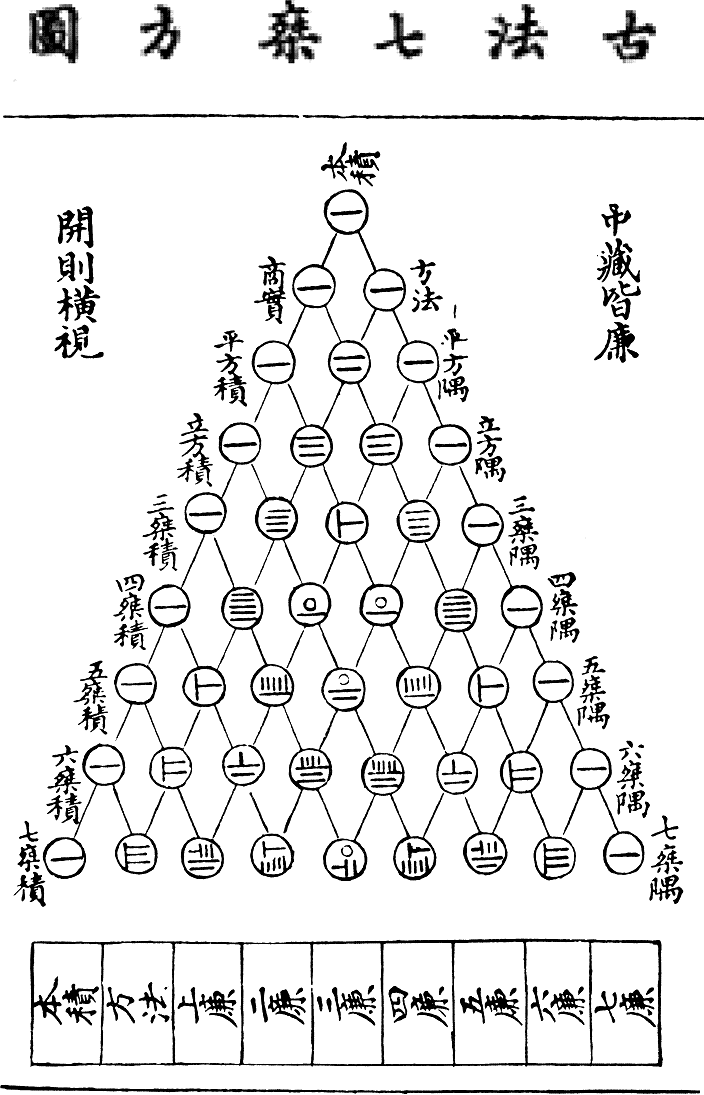
\includegraphics[width=.8\textwidth]{Yanghui_triangle}}{Треугольник Яна Хуэя, 1303}

\textbf{Задача.} Черепашка Пося находится в нижнем левом углу таблицы $(n+1)\times (m+1)$. За один ход Пося может переползти на одну клетку вверх или на одну клетку вправо. Сколько существует способов добраться до верхнего правого угла таблицы?

\begin{problems}
 
\item а) Пронумеруем строки от 1 до $(n+1)$, столбцы от 1 до $(m+1)$. Пусть черепашка начинает движение из клетки $(1, 1)$. Докажите, что количество способов добраться до клетки $(x, y)$ равно количеству способов добраться до клетки $(x-1, y)$ плюс количество способов добраться до клетки $(x, y-1)$.\\
б) Решите задачу про черепашку для $n=m=5$.

\item а) Мы выдрессировали черепашку. Теперь мы ей говорим, когда ползти вверх, а когда ползти вправо. Чтобы запомнить как именно черепашка ползёт, мы записываем очередность наших команд. Сколько вариантов записей могло получиться, если черепашка в итоге оказалась в клетке $(n+1, 2)$?\\
б) Решите задачу про черепашку Посю.

\item Посмотрите, куда черепашка может доползти за $n$ шагов и докажите тождество:
$$C_n^0+C_n^1+\cdots+C_n^n=2^n.$$

\item Пока мальчик Вова командует черепашкой, мальчик Лёня начал раскрывать скобки выражения:
$$(a+b)^n=(a+b)(a+b)\cdots (a+b).$$
Но получилось так, что когда Лёня умножал слагаемое на $a$, то Вова говорил черепашке ползти вверх, а если Лёня умножал слагаемое на $b$, то Вова говорил черепашке ползти вправо. В конце концов Лёня привел подобные слагаемые. Выразите получившиеся коэффициенты. 
\end{problems}

Запишем в каждую клетку таблицы число, равное количеству способов добраться до этой клетки. Повернем нашу таблицу так, чтобы все числа, отвечающие за одинаковое количество ходов, были на одном уровне. Результат называется \textbf{треугольником Паскаля}.

На краях этого треугольника стоят единицы, а каждое число внутри является суммой двух, стоящих над ним. $k$-е число $n$-й строки треугольника Паскаля равно $C_n^k$ (строки нумеруются сверху вниз, начиная с нуля, а числа в строках нумеруются слева направо, также начиная с нуля).

\begin{figure}[h!]
\center{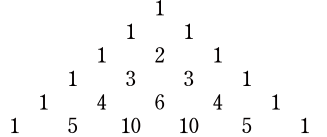
\includegraphics[scale=0.5]{pasc.png}}
\end{figure}

Коэффициенты разложения из 4 задачи называются \textbf{бином Ньютона.}
% \newpage
\begin{problems}
\item Вычислите выражение $C_n^0-C_n^1+C_n^2-\cdots\pm C_n^n$\\
а) используя треугольник Паскаля;\\
б) используя бином Ньютона.

\item У Тома Сойера есть забор из $2n$ досок и белая краска. Сколькими способами он может покрасить в этом заборе четное число досок?

\item Чему равно $C_k^k+C_{k+1}^k+\cdots+C_n^k$?

\item а) Для каждой из первых 4 строчек треугольника Паскаля сложите квадраты стоящих в ней чисел и найдите полученное число в треугольнике Паскаля. Запишите полученное тождество.\\
б) Докажите это тождество.
\end{problems}

\textbf{Числа Фибоначчи}~--- последовательность чисел:
$$1, \;1, \;2, \;3, \;5, \;8, \;13, \;21, \;34, \;55, \;89,\dots,$$
удовлетворяющая условию $F_0=1, F_1=1, F_{n+2}=F_{n+1}+F_n.$

\begin{problems}
\item Используя треугольник Паскаля докажите тождество: $$F_n=C_n^0+C_{n-1}^1+C_{n-2}^2+\cdots.$$
\end{problems}

\resetproblem
\vspace{1cm}
\addcontentsline{toc}{abcd}{\bf Матбой-междусобой. 12 июля}
\tolerance = 1600

\begin{center}
\textbf{\Large МеждусоБой}\\
\textit{12.07.16}
\end{center}

\begin{enumerate}
\item Через вершину $A$ параллелограмма $ABCD$ провели прямую $\ell$, пересекающую сторону $BC$. Докажите, что расстояние от точки $D$ до прямой $\ell$ равно сумме расстояний от точек $B$ и $C$ до этой же прямой. 
%легкая

\item В $10$ коробках лежат камни: в $k$-ой коробке лежит $2016+k$ камней ($k=~1,2,\ldots,10$). Двое играют в такую игру: один из игроков выбирает любые $5$ коробок и вынимает из них некоторое ненулевое количество камней (возможно, для разных коробок число вынутых камней различается, но для каждой из этих пяти коробок оно ненулевое). Тот, кто не может сделать ход, проигрывает. Кто из игроков выигрывает при правильной игре?
%средне-легкая 

\item На сторонах $AB$ и $BC$ равностороннего треугольника $ABC$ взяты точки $D$ и $E$ такие, что $AD = BE$. Отрезки $CD$ и $AE$  пересекаются в точке $O$. Серединный перпендикуляр к отрезку  $CO$ пересекает прямую $AO$ в точке $K$. Докажите, что $BK$ и $CO$ параллельны.
%средняя

\item По окружности расставлены в некотором порядке числа от 1 до 100. 
Назовем пару чисел {\it хорошей}, если эти два числа не стоят рядом, и хотя бы 
на одной из двух дуг, на которые они разбивают окружность, все числа 
меньше каждого из них. Чему может равняться общее количество хороших пар?
%тяжелая

\item На доске написано число 2000. Разрешается переставить в нем произвольным образом первые три цифры (ставить цифру 0 на первое место нельзя) или прибавить 361. Через 100 таких операций вновь получили 2000. Сколько раз прибавляли 361, если известно, что это сделали хотя бы один раз? 
%средне-тяжелая

\item Клетки шахматной доски $8 \times 8$ раскрашены в белый и черный цвета таким образом, что в каждом квадрате $2 \times 2$ половина клеток черные и половина белые. Сколько существует таких раскрасок?
%средне-тяжелая

\item В ряд выписано 25 цифр. Разрешается ставить между ними плюс, минус, умножить и скобки (склеивать цифры нельзя). Докажите, что всегда можно получить ноль.
%тяжелая

\item Компания из нескольких друзей вела переписку так, что каждое письмо получали все, кроме отправителя. Каждый написал одно и то же количество писем, в результате чего всеми вместе было получено 440 писем. Сколько человек могло быть в этой компании?
%легкая
\end{enumerate}

\resetproblem
\vspace{1cm}
\addcontentsline{toc}{abcd}{\bf Индукция-2. 14 июля}
\begin{center}
\textbf{\Large Индукция-2}\\
\textit{14.07.16}
\end{center}

\epigraph{\it Элемент тока длины $dl$ создаёт поле с магнитной индукцией $dB = k\frac{Idl}{r^2}$.}{Закон Био-Савара-Лапласа}

{\bf Задачи на разбор}
\begin{problems}

\item Плоскость поделена на области несколькими прямыми. Докажите, что эти области можно раскрасить в два цвета так, чтобы любые две соседние области были раскрашены в различные цвета.
\item У бородатого многоугольника во внешнюю сторону растет щетина. Его пересекает несколько прямых, на каждой из которых с одной из сторон тоже растет щетина. В результате многоугольник оказался разбитым на некоторое число частей. Докажите, что хотя бы одна из частей окажется бородатой снаружи (никакие три прямые не проходят через одну точку).
\item Докажите, что $3^{2n+2}+8n-9$ делится на 16.
\item Докажите, что любое число можно представить в виде суммы степеней двоек единственным образом.

\end{problems}
\resetproblem

{\bf Задачи для самостоятельного решения}
\begin{problems}
\item
Докажите равенство $$3 + 33 + 333 + \ldots + \underbrace{33 \ldots 33}_n = \dfrac{10^{n+1} - 9n - 10}{27}.$$
\item Числа вида $F_n = 2^{2^n} + 1$ называются числами Ферма. Докажите, что десятичная запись числа $F_n$ при $n \geqslant 2$ оканчивается цифрой 7.
\item Треугольник разбит на несколько частей несколькими прямыми. Докажите, что хотя бы одна из частей является треугольником.
\item Доказать, что монетами по 3 и 5 рублей можно выдать любую сумму больше 8 рублей?
\item Проведём в выпуклом многоугольнике некоторые диагонали так, что никакие две из них не пересекаются (из одной вершины могут выходить несколько диагоналей). Доказать, что найдутся по крайней мере две вершины многоугольника, из которых не проведено ни одной диагонали.
\item Докажите, что все числа 10017, 100117, 1001117, \ldots делятся на 53.
\item На столе стоят $2^n$ стаканов с водой. Разрешается взять любые два стакана и уравнять в них количества воды, перелив часть воды из одного стакана в другой. Докажите, что с помощью таких операций можно добиться того, чтобы во всех стаканах было поровну воды. 
\item Кусок бумаги разрешается рвать на 4 или на 6 кусков. Докажите, что по этим правилам его можно разорвать на любое число кусков, начиная с шести.
\item Докажите, что любое число можно представить в виде суммы нескольких различных чисел Фибоначчи. Единственно ли такое представление?
\item На кольцевой дороге стоят $n$ машин. При этом, суммарное количество топлива у машин  равно количеству топлива чтобы проехать один круг. Докажите, что существует машина, которая может проехать весь круг, забирая топливо у других машин.
\item Докажите, что $3^{2^n} - 1$ делится на $2^{n+2}$, но не делится на $2^{n+3}$.

\strut\hrule

\item Докажите, что $3^{2^n} - 1$ делится на $2^{n+2}$, но не делится на $2^{n+3}$.
\item Докажите,  что любое количество квадратов можно разрезать на несколько частей, из которых можно составить квадрат.
\item Даны два взаимнопростых числа $m$ и $n$, а также число 0. Имеется калькулятор, который умеет выполнять лишь одну операцию: вычислять среднее арифметическое двух чисел одной чётности. Докажите, что с помощью этого калькулятора можно получить все числа от $1$ до $n$.
\item  На окружности взяли $n$ точек и соединили их всевозможными отрезками. Оказалось, что никакие три не пересекаются в одной точке. На сколько частей они делят круг?
\end{problems}

\resetproblem
\vspace{1cm}
\addcontentsline{toc}{abcd}{\bf Симметрия. 14 июля}
\tolerance = 1600

\begin{center}
\textbf{\Large Симметрия}\\
\textit{14.07.16}
\end{center}

\epigraph{\it Неочевидное, \\ Невероятное, \\ Но явно что-то неземной красоты...}{Л. Агутин, ``Мир зелёного цвета''}

\begin{problems}
\item Внутри острого угла с вершиной $O$ взяли произвольную точку $A$. Её отразили относительно сторон угла и получили точки $A_1$ и $A_2$. Докажите, что угол $A_1OA_2$ не зависит от выбора точки.

\item а) Точки $A$ и $B$ лежат по одну сторону от прямой. Постройте на этой прямой такую точку $M$, чтобы отрезки $AM$ и $BM$ образовывали с данной прямой равные углы.

б) То же самое, но $A$ и $B$ должны лежать по разные стороны от прямой.

\begin{center}
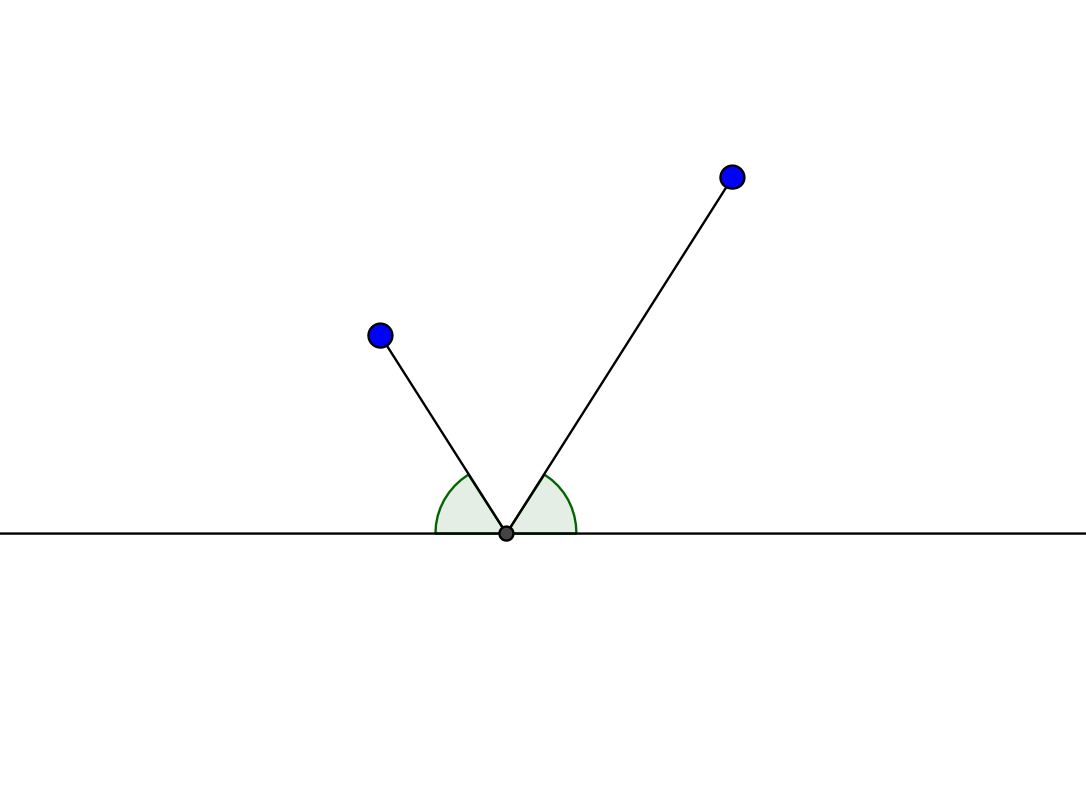
\includegraphics[width=.35\textwidth]{simm01}
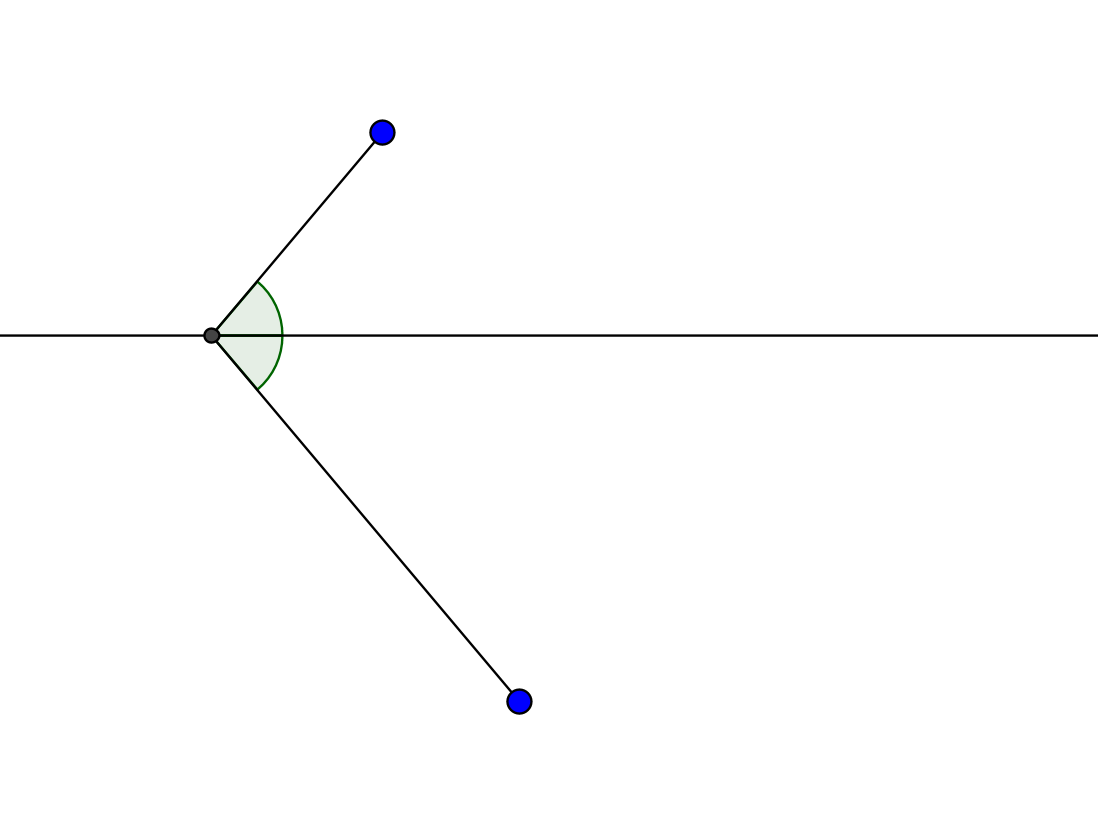
\includegraphics[width=.35\textwidth]{simm02}
\end{center}

\item а) В выпуклом четырёхугольнике $ABCD$ угол $A = 30^\circ$. Докажите, что ${AC \leqslant BC + CD + DB}$.

б) В выпуклом четырёхугольнике $ABCD$ угол $A$ прямой. Докажите, что ${2AC \leqslant BC + CD + DB}$.

\item Точка $M$~--- середина гипотенузы $AB$ прямоугольного треугольника $ABC$, угол $B$ которого равен $30^\circ$. На его катете $BC$ выбирают такую точку $K$, что $AK + KM = BC$. Докажите, что $MK\perp AB$.

\item На гипотенузе $AB$ и катете $BC$ прямоугольного равнобедренного треугольника $ABC$ соответственно взяли произвольные точки $M$ и $K$. Докажите, что $AK + KM \geqslant AB$.

%\item Из точки, лежащей на диаметре полукруга, под равными к нему углами провели два отрезка так, как показано на рисунке. Докажите, что сумма этих отрезков не больше диаметра полукруга.

\item На стороне $BC$ треугольника $ABC$ выбрана точка $D$. Кроме этого $$\angle{BAC}:\angle{ADC}:\angle{BCA}=3:2:1.$$ 
При этом $BC=19, AB=13$. Найдите $AD$.

\item В прямоугольнике $ABCD$ точка $M$~--- середина стороны $BC$, точка $N$~--- середина стороны $CD$, $P$~--- точка пересечения отрезков $DM$ и $BN$. Докажите, что угол $MAN$ равен углу $BPM$.

\item Биссектриса $AE$ равнобедренного треугольника $ABC$ ($AB = BC$) пересекает биссектрису его угла $B$ в точке $O$. На боковой стороне $AB$ взяли точку $M$ так, что $AM = AC$. Прямая $MO$ пересекает основание $AC$ в точке $K$. Докажите, что $AK = EC$.

%\item Внутри треугольника взяли произвольную точку. Всегда ли можно провести через неё три прямые так, чтобы отрезок каждой из них внутри треугольника делился данной точкой пополам?

\end{problems}
\resetproblem
\vspace{1cm}
\addcontentsline{toc}{abcd}{\bf Алгоритм Евклида. 15 июля}
\begin{center}
\textbf{\Large   Алгоритм Евклида }\\
%\textit{Профи}\\
\textit{15.07.16}
\end{center}

\epigraph{\it То, что принято без доказательства, может быть отвергнуто без доказательства.}{Евклид}

\indent \textbf{Определение 1.} \textit{Наибольшим общим делителем} двух целых чисел называется такой их общий делитель, который больше всех остальных общих делителей.\\
\indent \textbf{Определение 2.} \textit{Наименьшим общим кратным} двух целых чисел называется наименьшее положительное число, делящееся на оба этих числа.\\
\textbf{Обозначение.} НОД$(a,b)=(a,b)$, НОК($a,b$)=[$a,b$].\\
\textbf{Определение 3.} Если $(a,b)=1$, то числа $a$ и $b$ называются \textit{взаимно простыми}. 
\textbf{Алгоритм Евклида.}\\
Пусть $a$ и $b$ -- целые числа, не равные одновременно нулю, и последовательность чисел
$a > b > r_1 > r_2 > r_3 > r_4 > ... > r_n$
определена тем, что каждое $r_k$~-- это остаток от деления предпредыдущего числа на предыдущее, а предпоследнее делится на последнее нацело, то есть \\
\begin{equation*}
 a = b \cdot q_0 + r_1
\end{equation*}
\begin{equation*}
b = r_1  \cdot q_1 + r_2
\end{equation*}
\begin{equation*}
r_1 = r_2  \cdot q_2 + r_3
\end{equation*}
\begin{center} $\cdots$ \end{center}  
\begin{equation*}
r_{k-2} = r_{k-1}  \cdot q_{k-1} + r_k
\end{equation*}
\begin{center} $\cdots$ \end{center}
\begin{equation*}
r_{n-2} = r_{n-1}  \cdot q_{n-1}+ r_n
\end{equation*}
\begin{equation*}
r_{n-1} = r_n  \cdot q_n
\end{equation*}
Тогда $(a,b)=r_n$.\\
\textbf{Упражнение. } Найдите \textbf{a)} ($1333$, $372$);  \textbf{b)} ($561$, $4301$);   \textbf{c)} ($9163$, $3311$).



\begin{problems}
\item Докажите следующий свойства НОД и НОК:\\
\textbf{a)} если $m$ делится на $n$, то $(m$, $n)=n$, $[m$, $n]=m$;\\
\textbf{b)} $(a \cdot m$, $a \cdot n$)=$a\cdot (m$, $n)$;\\
\textbf{c)} если $(m$, $n)=d$, то $(\frac{m}{d}$, $\frac{n}{d})=1$;\\
\textbf{d)} для любого целого числа $a$ справедливо, что $(m$, $n$)=($m-a \cdot n$, $n)$;\\
\textbf{e)} $(m$, $n) \cdot [m$, $n]=m\cdot n$.
\item \textbf{a)} Докажите, что ($n+3$, $5n+14$)  взаимно просты при любом целом $n$.\\  
\textbf{b)} Какие значения может принимать ($3n+2$, $10n+23$).
\item Вася посчитал НОК всех чисел от $1$ до $1000$, а Петя -- всех чисел от $501$ до $1000$. У кого результат получился больше и во сколько раз?

\item Пусть $m,n$ -- целые взаимнопростые числа. Найдите наибольшее возможное значение $(n+2016m$, $m+2016n)$.

\item Пусть $a$ и $b$ -- натуральные числа. Докажите, что среди чисел $a, 2a, 3a,...,ba$ ровно ($a$, $b$) чисел делится на $b$.

\item Изначально на доске записаны числа $m$ и $n$. Каждую минуту Саша записывает в тетрадку квадрат наименьшего из чисел на доске, после чего Даша ищет разность чисел на доске и записывает ее вместо наибольшего из них, пока в какой-то момент не выпишет $0$. Чему равна сумма  чисел у Саши в тетради?

\item Пусть $a$ и $b$ –- взаимно простые натуральные числа. В доме есть лифт с двумя кнопками, одна из которых
поднимает лифт на $a$ этажей вверх, а вторая опускает на $b$ этажей вниз, если это возможно (например, на последнем этаже первая кнопка не работает). Докажите, что на этом лифте можно попасть с любого этажа на любой другой, если высота дома не меньше
\textbf{а)} $2ab$; \textbf{б)} $a + b$.

%\item Натуральные числа $a, b$ и  $c$ удовлетворяют равенству:
%\begin{equation*}
%[a,c]-[b,c]= a-b
%\end{equation*}
%Докажите, что $a$, $b$ делятся на $c$. 
%Докажите, что в вершинах любого графа можно расставить натуральные числа так, что любые два числа,
%соединенные ребром имеют НОД>1, а числа, не соединенные ребром, взаимно просты.

\end{problems}

\begin{center}
\textbf{Перегородка}
\end{center}

\begin{problems}
\item На доске написаны взаимнопростые числа $m$ и $n$. Каждую минуту модуль разности этих чисел записывается вместо наибольшего из них. Докажите, что в какой-то момент на доске будут написаны две единицы. 
\item Пусть $p$~--- простое число. Сколько существует пар взаимнопростых натуральных чисел $(m,n)$ таких, что $p=m+n$? 
\item Аня нашла себе интересное занятие. Она написала на доске две единички, потом между ними написала их сумму. Ее это так захватило, что она продолжила: брала ряд чисел, который у нее получился на предыдущем шаге, и между двумя соседними числами писала их сумму (старые числа при этом не стирала).\\ \textbf{a)} Сколько раз она выписала простое число $p$?\\  \textbf{b)} Сколько раз она выписала произвольное число $n$? 

\end{problems}

\resetproblem
\vspace{1cm}
\addcontentsline{toc}{abcd}{\bf Изоморфизм комбинаторных задач. 15 июля}
\begin{center}
\textbf{\Large Изоморфизм комбинаторных задач}\\
%\textit{Профи}\\
\textit{15.07.16}
\end{center}

\epigraph{\it Если $666$~--- это зло, то $25.807$~--- корень зла.}{Народная мудрость}

Не решая задач, разбейте их на группы <<одинаковых задач>>. Объясните, как установить соответствие между задачами одной группы.

\begin{problems}

\item Зуб может быть здоровым, больным, отсутствующим, растущим, искусственным и сломанным. У шушканчиков 6 рядов по 6 зубов. К черепашке Посе пришли в гости несколько шушканчиков с различными наборами зубов. Каково могло быть максимальное число гостей-шушканчиков? % 6^36

\item Сколькими способами можно поставить на доску $6\times6$ шесть ладей? % C

\item Сколько существует способов расставить 36 человек в шеренгу? % !

\item Сколькими способами можно на доске $36\times36$  расставить 36 ладей, не бьющих друг друга? % !

\item Есть 36 человек. Сколькими способами можно разбить их на 6 команд по 6 человек, если команды будут участвовать в разных соревнованиях? % multiC

\item Пося приехала в страну, где всего 64 города: каждый из них называется словом из 6 букв, состоящим только из букв <<Х>> и <<Е>>. Дорогой соединены ровно те пары городов, названия которых отличаются ровно в одной букве. Пося вышла из города ХХХХХХ и 36 раз прошла по дороге в другой город. Сколькими способами она могла это сделать? % 6^36

\item В магазине продаются чашки 6 видов и блюдца 6 видов. Сколькими способами можно выбрать 6 различных наборов из чашки и блюдца? % C

\item Имеется 30 ёжиков и 6 дикобразов. Сколько существует способов отправить по одному зверьку в 36 зоопарков? % C

\item Сколькими способами можно расставить на доске $6\times6$ числа от 1 до 36? % !

\item У Поси есть 6 револьверов, каждый из которых содержит по 6 пуль. Пули в первом револьвере отравляют, во втором~--- разрывают, в третьем~--- пронзают насквозь, в четвёртом~--- поджигают, в пятом~--- отчисляют из лагеря, а в шестом~--- расщепляют на молекулы. Пося хочет расстрелять 36 черепах по очереди: сначала первую, затем вторую, и так далее. Каждый выстрел можно делать из любого револьвера, в котором на этот момент есть хотя бы одна пуля. Сколькими способами Пося может это сделать? % multiC

\item В алфавите ЛМШ есть 6 букв: <<л>>, <<м>>, <<ш>> и <<ф>>, <<x>>, <<б>>. Сколько различных слов длины 36 есть в ЛМШ (любая последовательность букв в ЛМШ считается осмысленной)? % 6^36

\item Сколько существует способов раскраски доски $6\times6$ в 6 цветов? % 6^36

\item Есть 6 видов конфет, по мешку каждого вида. Сколько существует способов угостить ими 6 девочек так, чтобы ни одной не попалось более пяти одинаковых конфет? % 6^36

\item Есть 36-угольник, сколько существует шестиугольников с вершинами в вершинах 36-угольника? % C

\item Есть 36 разных конфет. Сколькими способами можно раздать их 36 девочкам по одной? % !

\item В стране черепашки Поси 117649 городов: Вишкиль-000000, Вишкиль-000001, и так далее до Вишкиля-666666 (в записи каждого используются только цифры от 0 до 6). Дорогой соединены ровно те пары городов, которые отличаются ровно в одной цифре на 1. Пося вышла из города Вишкиль-000000 и, двигаясь только по дорогам, посетила некоторые города в порядке возрастания номеров и остановилась в Вишкиле-666666. Сколькими способами она могла это сделать? % multiC

% \item (переделать)
% Черепашка Пося ходит по городу, в котором к каждому перекрёстку ведёт одна дорога, а отходит по 6. Пося собирается делать выбор на 6 перекрёстках. Сколько есть различных мест, куда она может попасть?
% \item (переделать)
% У Поси есть 6 волшебных игральных кубиков. Если такой кубик подкинуть, то результат выпадения повторится не раньше чем через сутки (если кубик не может выпасть ни на одну из граней, он испаряется). Пося достаёт кубики из мешочка, подкидывает, запоминает результат и возвращает в мешочек. Сколькими способами она может это сделать, пока все кубики не испарятся?

\end{problems}
\resetproblem
\vspace{1cm}
\addcontentsline{toc}{abcd}{\bf Перекладывание отрезков. 16 июля}
\begin{center}
\textbf{\Large Перекладывание отрезков}\\
\textit{16.07.16}
\end{center}

\epigraph{\it Выживает только сильнейший.}{Ч. Дарвин}

\begin{problems}
\item На катетах $AC$ и $BC$ равнобедренного прямоугольного треугольника отметили точки $M$ и $L$ 
соответственно так, что $MC=BL$. Точка $K$ --- середина гипотенузы $AB$. Докажите, что треугольник 
$MKL$ также является прямоугольным равнобедренным. 

\item В треугольнике $ABC$ биссектриса $AE$ равна по длине отрезку $EC$. Причем $2AB=AC$. Найдите 
углы треугольника $ABC$.

\item В равнобедренном прямоугольном треугольнике $ABC$ на гипотенузе $AB$ взяты точки $M$ и $N$ ($N$ между $M$ и $B$) такие, что $\angle MCN=45^{\circ}$. Докажите, что из отрезков $MN, AM, NB$ можно составить прямоугольный треугольник.

\item В равнобедренном треугольнике $ABC\; (AB = BC)$ на боковую сторону $BC$ опущена высота $AH$. Точка $L$~--- основание перпендикуляра из $H$ на сторону $AB$. Оказалось, что $AL = AB/4$. Найдите углы треугольника $ABC$.
%легко, счет углов

\item На боковых сторонах $AB$ и $AC$ равнобедренного треугольника $ABC$ отметили соответственно точки $K$ и $L$ так, что $AK = CL$ и $\angle ALK + \angle LKB = 60^{\circ}$. Докажите, что $KL = BC$.

\item На гипотенузе~$AC$ прямоугольного треугольника $ABC$ выбрали точку~$D$ такую, что $BC=CD$. На катете~$BC$ выбрали такую точку~$E$, что $DE=CE$. Докажите, что $AD+BE=DE$. 
% На равенство треугольников с доп построением

\item В квадрате $ABCD$ точки $K$ и $M$ принадлежат сторонам $BC$ и $CD$  соответственно, причем $AM$~--- биссектриса угла $\angle KAD$. Докажите, что $AK=DM+BK$.

%\item В равнобедренном треугольнике $ABC$ с основанием $AC$ проведена биссектриса $AD$. Известно, что $AD+BD = AC$. Найдите углы треугольника.
%трудновато, надо правильно отложить пару отрезков и потом считать углы

\item На медиану $BM$ треугольника $ABC$ опустили перпендикуляр $AL$ и перпендикуляр $DK$ из некоторой точки $D$ на стороне $AB$ ($L$ и $K$~--- различные точки, лежащие внутри $BM$). Оказалось, что $BK = LM$. Докажите, что $CD = BD+BA$.
%удвоение медианы, внимательно смотреть, не очень легко

\end{problems}
\resetproblem
\vspace{1cm}
\addcontentsline{toc}{abcd}{\bf Линейное представление НОД. 16 июля}
\begin{center}
\textbf{\Large   Линейное представление НОД }\\
%\textit{Профи}\\
\textit{16.07.16}
\end{center}

\epigraph{\it Не всё в жизни смешно.}{Р. Л. Асприн}
 
\begin{problems}
\item Натуральные числа $a$ и $b$ взаимно просты. По окружности длины $a$ катится колесо
длины $b$, в обод которого вбит гвоздь, оставляющий на окружности отметины.\\
\textbf{a)} Докажите, что в какой-то момент новые отметины перестанут появляться.\\
 \textbf{b)} Докажите, что в этот момент отметины делят обод неподвижного колеса на равные части.\\ 
\textbf{c)} Пусть $c$~--- длина отрезка между двумя соседними отметинами. Докажите, что $c=1$.\\ 
\textbf{d)} \textbf{(Линейное представление НОД)} Докажите, что существуют целые числа $m$ и $n$ такие, что $m a+n b=1$.\\
\textbf{e)} Докажите, что для произвольных чисел $a$ и $b$ (не обязательно взаимнопростых) существуют целые числа $m$ и $n$, такие что $am+bn=(a,b)$.
\item В государстве имеют хождение монеты достоинством $a$ и $b$ золотых, где $a$ и $b$ -- взаимнопростые натуральные числа. Докажите, что такими монетами можно (возможно, со сдачей) набрать любую сумму.

\item Докажите, что угол в $17^{\circ}$ можно разделить с помощью циркуля и линейки на $17$ равных частей.

\item В классе химии имеются $25$ пробирок объема $1$, $2$, \ldots, $25$ мл. Когда химики стали собираться в ЛМШ, оказалось, что у них осталось мало места, и они могут взять только набор из $10$ пробирок. Химики хотят, чтобы с помощью любых двух пробирок из набора можно было отмерить $1$ мл. Сколькими способами можно составить такой набор?

\item Петя произвольным образом разложил некоторое количество монет по $30$ коробкам.
Вася может выбрать любые $k$ коробок и добавить в каждую из них по монете. При каких
$k$ Вася такими операциями сможет при любом исходном раскладе уравнять число монет
во всех коробках?

\item \textbf{a)} Числа $a$, $b$ и $c$ взаимнопросты в совокупности, то есть $(a,b,c)=1$.\\
Докажите, что любое число $d$ можно представить в виде $d=ax+by+cz$, где $x$, $y$, $z$~--- целые.\\
\textbf{b)} Сформулируйте и докажите аналогичную задачу, если изначально дано $n$ чисел, взаимнопростых в совокупности.

\item Докажите, что для любых натуральных чисел $a$ и $b$ существуют такие натуральные числа $c$ и $d$, что числа $an+c$ и $bn+d$ взаимнопросты при всех натуральных $n$.

%\item На доске написано четыре числа $m$, $n$, $m$, $n$. Каждую минуту с числами проделывается следующая операция: если на доске записаны $x$, $y$, $z$, $t$ и $x>y$, то все числа стираются и вместо них записываются $x-y$, $y$, $z+t$, $t$, а если $x<y$, то вместо них записываются $x$, $y-x$, $z$, $t+z$. Через несколько минут первые два числа стали равны. Докажите, что сумма двух последних равна $2mn$. 

\end{problems}
%\item Натуральные числа $a, b$ и  $c$ удовлетворяют равенству:
%\begin{equation*}
%[a,c]-[b,c]= a-b
%\end{equation*}
%Докажите, что $a$, $b$ делятся на $c$. 
%Докажите, что в вершинах любого графа можно расставить натуральные числа так, что любые два числа,
%соединенные ребром имеют НОД>1, а числа, не соединенные ребром, взаимно просты.

\resetproblem
\vspace{1cm}
\addcontentsline{toc}{abcd}{\bf Дискретная непрерывность. 17 июля}
\renewcommand{\baselinestretch}{0.8}
\parskip=0.75\parskip

\begin{center}
\textbf{\Large Дискретная непрерывность}\\
\textit{17.07.16}
\end{center}

\epigraph{\it --- Я ранее бывал в этом городе, тогда даже ни одной гостиницы не было. А теперь сразу две и с интересными названиями!}{С. Карамов, ``Бег на месте, или замкнутый круг''}

Разбор.
В ряд выложены 100 черных и 100 красных шаров, причём самый левый и самый правый шары чёрные. Докажите, что можно выбрать слева подряд несколько шаров (но не все!) так, чтобы среди них количество красных равнялось количеству чёрных. 

\begin{problems}
\item Шеренга новобранцев стояла лицом к сержанту. По команде ``налево'' некоторые повернулись налево, некоторые~--- направо, а остальные~--- кругом. Всегда ли сержант сможет встать в строй так, чтобы с обеих сторон от него оказалось поровну новобранцев, стоящих к нему лицом? 

\item За круглым столом сидит 10 мальчиков и 10 девочек. Докажите, что найдётся группа из 10 сидящих подряд детей, в которой девочек и мальчиков поровну. 

\item
Существуют ли сто последовательных натуральных чисел, среди которых
ровно пять простых?

%\item   Некто   расставил   в   произвольном   порядке   десятитомное   собрание   сочинений.
%Назовем <<беспорядком>> пару томов (не обязательно соседних), в которой том с большим
%номером стоит левее. Для некоторой расстановки томов подсчитано количество всех
%<<беспорядков>>. Какие значения оно может принимать? 

\item За круглым столом сидит чётное количество гномов. У каждого на колпаке по несколько помпонов. Причём у любых двух рядом сидящих гномов количество помпонов отличается не более чем на 1. Докажите, что найдётся пара гномов, сидящих друг напротив друга, количества помпонов на колпаках которых отличаются не больше, чем на 1.

\item      В зале находятся $n$ юношей и $n$ девушек, причём никакие трое не находятся на одной прямой. Всегда ли можно провести по полу прямую черту так, чтобы в каждой из образовавшихся частей зала юношей и девушек было поровну (но не ноль)? 

\item Грани восьми единичных кубиков окрашены в чёрный и белый цвета так, что чёрных и белых граней поровну. Докажите, что из этих кубиков можно сложить куб со стороной 2, на поверхности которого чёрных и белых квадратиков поровну.

\item В ряд стоят $n$ шаров, известно, что среди этих шаров могут быть шары только двух цветов: чёрного и белого. Если в автомат отправить запрос $(a, b)$, то он проверит шары на местах с номерами $a$ и $b$ и если первый чёрный, а второй~--- белый, то поменяет их местами. Паша утверждает, что может, не зная исходного набора, написать такой список запросов, что потом на двух, известных ему позициях, будут шары одного цвета. Докажите, что Паша хвастается безосновательно.  


\end{problems}

\renewcommand{\baselinestretch}{1}
\parskip=1.25\parskip

\resetproblem
\vspace{1cm}
\addcontentsline{toc}{abcd}{\bf Точки пересечения биссектрис. 19 июля}
\begin{center}
\textbf{\Large Точки пересечения биссектрис}\\
\textit{19.07.16}
\end{center}

\epigraph{\it две параллельные прямые\\
живут в евклидовом мирке\\
и бегают пересекаться\\
в мир лобачевского тайком}{Пирожок}

\begin{problems}
\item В треугольнике $ABC$ $\angle A=\alpha$. Найдите угол между биссектрисами $BB_1$ и $CC_1$.

\item Может ли точка пересечения биссектрис лежать на средней линии треугольника?

\begin{center}
	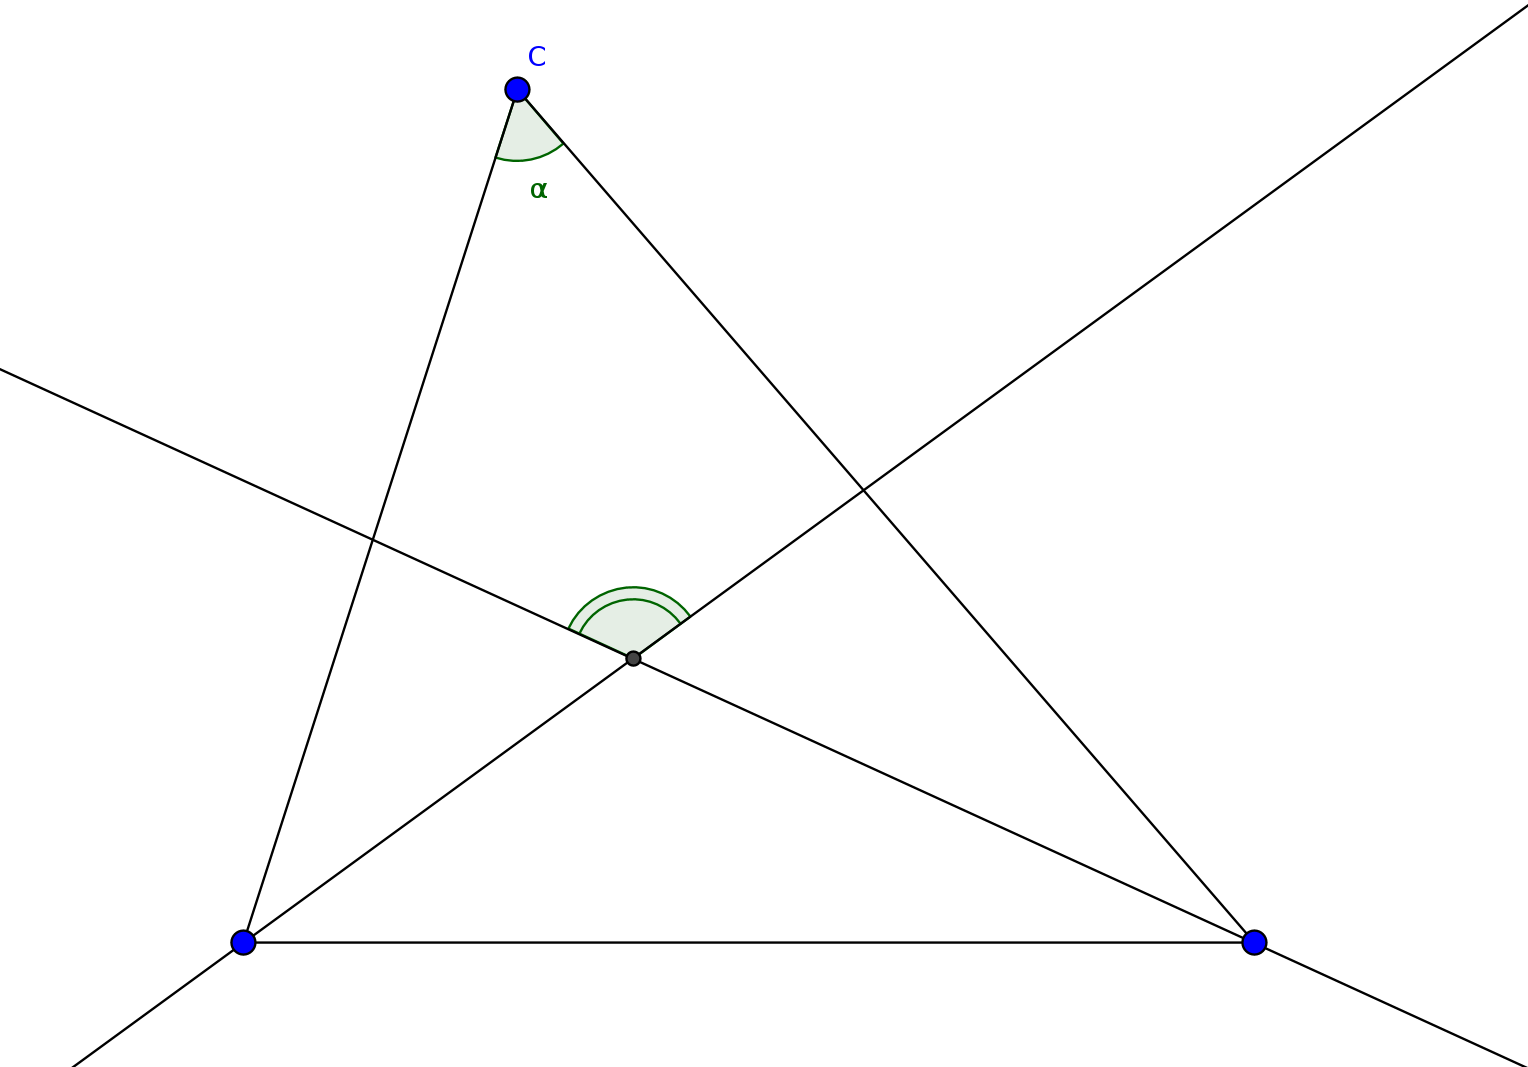
\includegraphics[width=.45\textwidth]{incen01}
	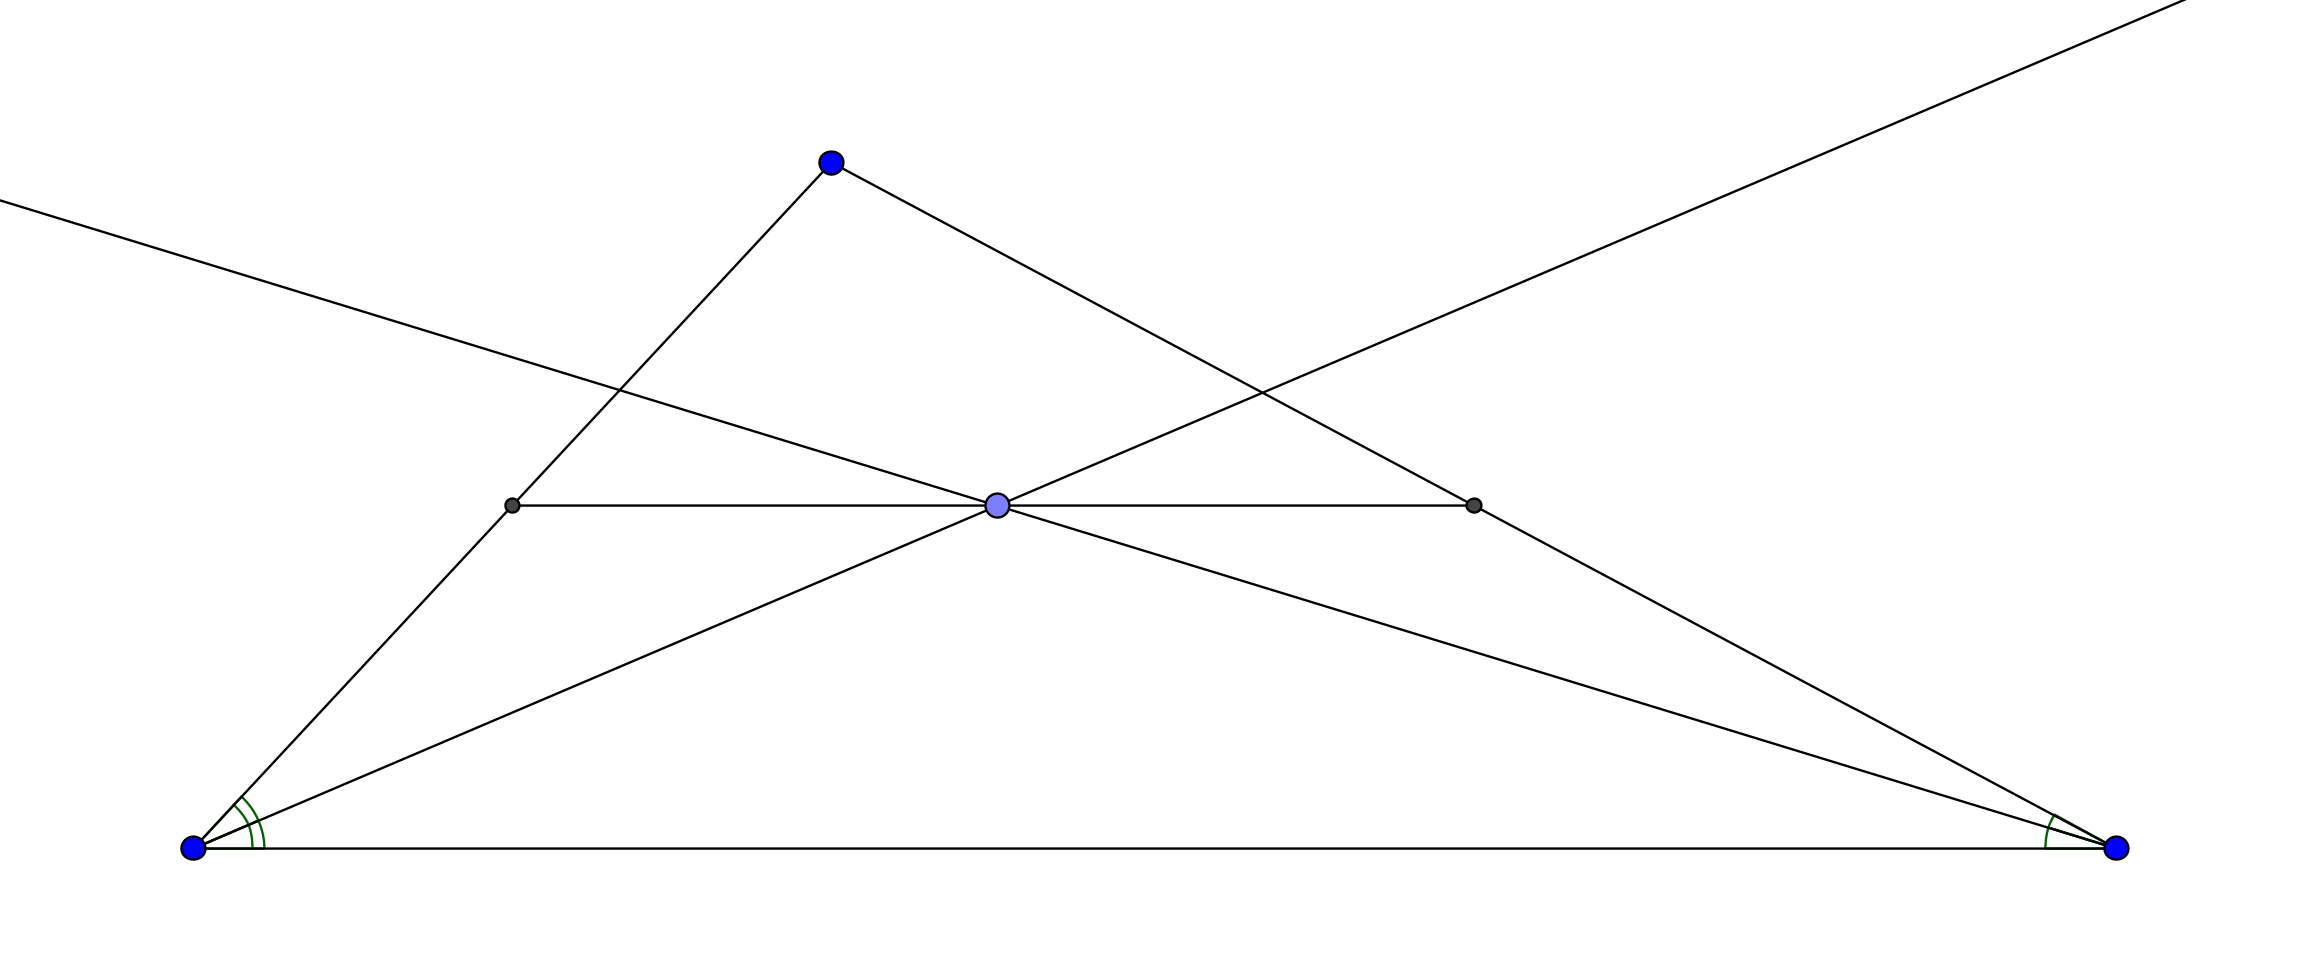
\includegraphics[width=.45\textwidth]{incen02}
\end{center}

\item В четырёхугольнике $ABCD$ $\angle B=\angle C=146^{\circ}$. Биссектриса угла $D$ пересекает серединный перпендикуляр к стороне $BC$ в точке $O$. Найдите $\angle AOD$.

\item В выпуклом шестиугольнике $ABCDEF$, все углы которого тупые, $\angle A=\angle B$, $\angle C=\angle D$, $\angle E=\angle F$. Докажите, что серединные перпендикуляры к его сторонам $AB, CD, EF$ пересекаются в одной точке.

\item Биссектрисы двух соседних углов четырехугольника пересекаются в середине его стороны. Докажите, что либо у этого четырехугольника равны два угла, либо две стороны параллельны. 

\item От угла равностороннего треугольника со стороной $1$ отрезали меньший треугольник так, что биссектриса его внешнего угла делит пополам сторону исходного треугольника, противоположную данному углу. Найдите периметр отрезанного треугольника.

\item Дан четырёхугольник $ABCD$, в котором $\angle ABD=\angle DBC=60^{\circ}$, $\angle ADB=40^{\circ}$, а $\angle BDC=70^{\circ}$. Найдите угол между его диагоналями.

\begin{center}
	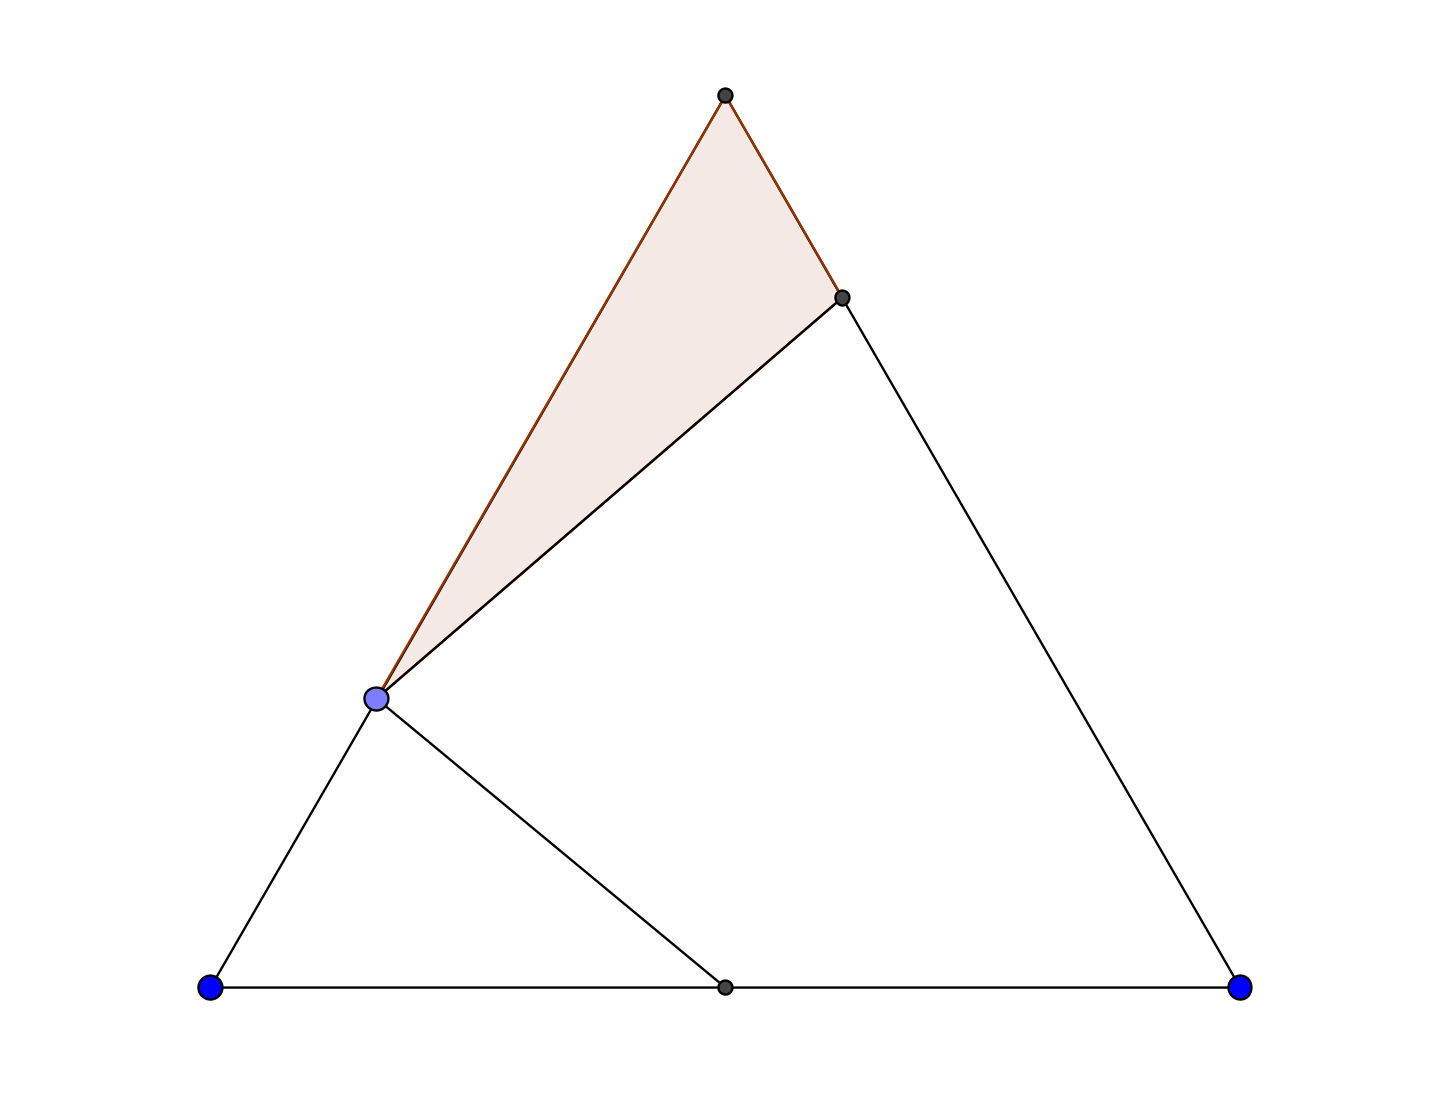
\includegraphics[width=.45\textwidth]{incen03}
	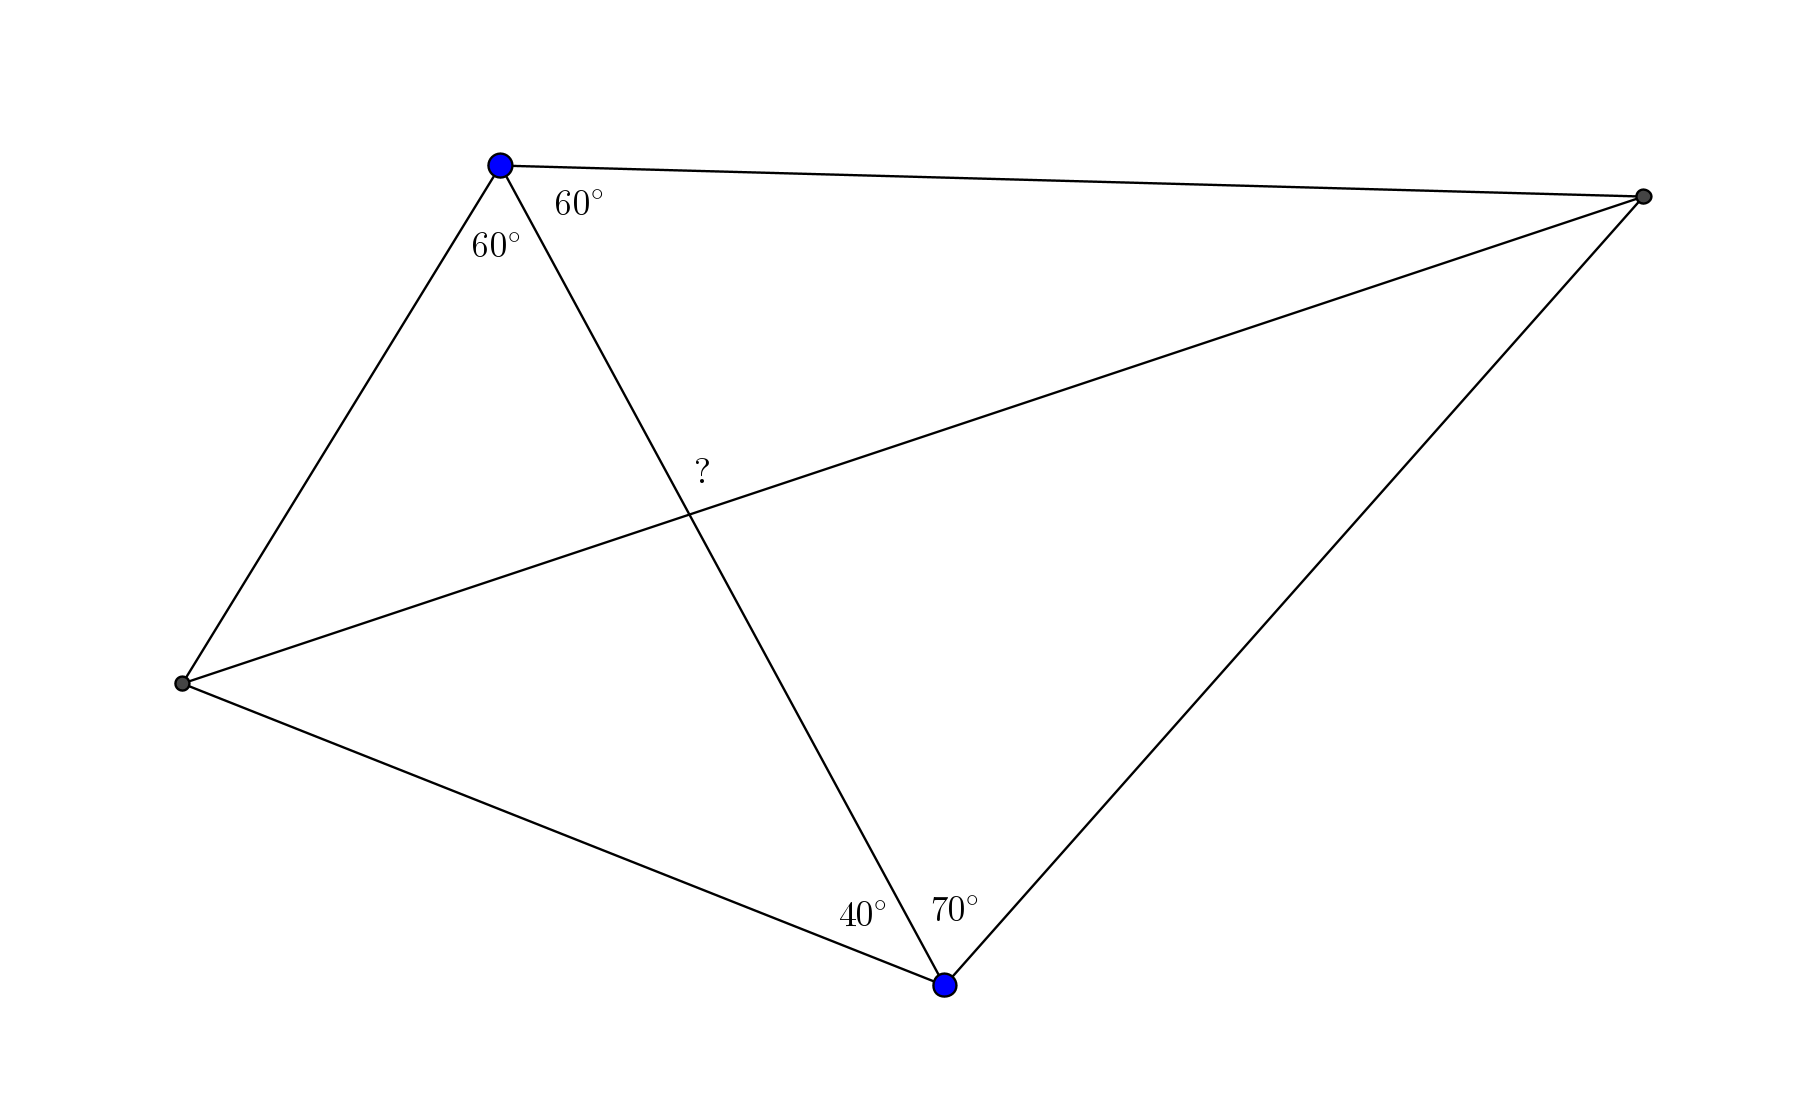
\includegraphics[width=.45\textwidth]{incen04}
\end{center}

\item В треугольнике $ABC$ угол $A$ равен $60^{\circ}$. На сторонах $AB$ и $AC$ выбраны точки $K$ и $L$ соответственно так, что $BK = KL = LC$. Докажите, что угол $KLC$ в два раза больше угла $ABC$.
%центр вневписанной окружности

%\item На~сторонах $AB$ и~$AD$ единичного квадрата $ABCD$ выбраны точки $N$ и~$P$ соответственно. Причем периметр треугольника $ANP$ равен 2. Докажите, что $\angle NCP=45^{\circ}$.

\end{problems}
\resetproblem
\vspace{1cm}
\addcontentsline{toc}{abcd}{\bf Индукция в графах. 19 июля}
\begin{center}
\textbf{\Large Индукция в графах}\\
\textit{19.07.16}
\end{center}

\epigraph{\it ...и, когда он уснул, взял одно из ребр его...}{Книга Бытия}

Разбор. Докажите по индукции, что в дереве с $n$ вершинами $n-1$ ребро.

\begin{problems}

\item
Усадьбы любых двух джентльменов в графстве Вишкиль соединены либо водным (лодочка), либо сухопутным (карета) сообщением. Докажите, что можно закрыть один из видов транспорта так, чтобы любой джентльмен мог по-прежнему добраться до любого другого.

\item В одном государстве 100 городов, и каждый соединён с каждым дорогой с односторонним движением. Докажите, что можно поменять направление движения не более, чем на одной дороге, так, чтобы от каждого города можно было доехать до любого другого.

\item В графе степень каждой вершины не превосходит $d$. Докажите, что все вершины графа можно покрасить в $d + 1$ цвет так, чтобы любые две вершины, соединённые ребром, имели разный цвет. 

%\item (вершины, средняя)
\item  а) Докажите, что в турнире (полном ориентированном графе) найдётся путь, который проходит по каждой вершине ровно один раз. \\
б) В шахматном турнире каждый сыграл с каждым по партии. Докажите, что участников можно перенумеровать так, что участник с номером $n$ не проиграл участнику с номером $n+1$.

\item Докажите, что граф двудольный, если в нем нет циклов нечётной длины, используя:\\
а) индукцию по количеству вершин;\\
б) индукцию по количеству ребер.

%\item (рёбра) формула Эйлера

\item На конференцию приехали учёные, каждый из них знает несколько языков. Оказалось, что любые трое человек могут поговорить друг с другом (возможно, одному из них придётся переводить для остальных). Докажите, что учёные могут разбиться на пары, говорящие на одном языке, если общее число учёных чётное.

\item В стране 100 городов и несколько дорог. Каждая дорога соединяет два каких-то города. Из каждого города можно добраться до любого другого, двигаясь по дорогам. Докажите, что можно объявить несколько дорог главными так, чтобы из каждого города выходило нечётное число главных дорог.

%дальше могут быть драконы
%\item (Вершины) Школьники играли в настольный теннис "на победителя". Они установили очередь и правила: вначале играют первый и второй, а в дальнейшем каждый очередной участник играет с победителем предыдущей пары. На следующий день те же школьники снова сыграли по тем же правилам, но очередь шла в обратном порядке (вчерашний последний стал первым, предпоследний – вторым, и так далее). Известно, что каждый сыграл хотя бы раз и в первый день, и во второй. Докажите, что найдутся два школьника, которые играли между собой и в первый день, и во второй.

%\item (вершины, конструктив, забава)$n$ человек не знакомы между собой. Нужно так познакомить друг с другом некоторых из них, чтобы ни у каких трех людей не оказалось одинакового числа знакомых. Докажите, что это можно сделать при любом $n$.

%\item (не добро, вершинки по три) Пусть в графе не менее чем  $3n - 2$  вершины и не более чем  $3n - 2$  ребра  ($n \geq 2$).  Тогда найдутся $n$ вершин, между которыми нет ребер. 

%\item (рёбра??) В стране некоторые пары городов соединены дорогами. Оказалось, что нет трёх городов, соединённых дорогами попарно. Кроме того, для любых $n$ дорог, найдётся город, из которого выходит хотя бы две из них. Докажите, что города можно так разбить на $n$ округов, что дорог внутри округов не будет.

%\item В компании из  $2n + 1$ человека для любых $n$ человек найдется отличный от них человек, знакомый с каждым из них. Докажите, что в этой компании есть человек, знающий всех.



\end{problems}
\resetproblem
\vspace{1cm}
\addcontentsline{toc}{abcd}{\bf Шары и перегородки. 20 июля}
\begin{center}
\textbf{\Large И снова комбинаторика}\\
%\textit{Профи}\\
\textit{20.07.16}
\end{center}

\renewcommand{\epigraphwidth}{.45\textheight}

\epigraph{\it Двумерная сфера~--- это граница трёхмерного шара, но гомотопически трёхмерный шар примитивен, он стягивается в точку, а сфера являет собой все тайны гомотопического хаоса.}{Роман Михайлов}

\begin{problems}

\item 
(а) Есть буквы Ш (12 штук) и П (5 штук). Сколькими способами можно их расставить?

(b) Есть Шары (12 штук) и Перегородки (5 штук). Сколькими способами можно их переставить?
 
(c) Есть 6 коробок и 12 одинаковых кубиков. Сколькими способами можно разложить кубики по коробкам?
 
(d) Игральную кость подкидывают 12 раз. Сколько различных вариантов есть?

\item 
(а) В магазине 5 касс и всего 10 покупателей. Сколькими способами они могут распределиться по очередям (очередь у любой кассы может быть любой длины, все кассы разные)? 

(b) В почтовом отделении продаётся 5 видов открыток. Сколькими способами можно купить 10 открыток?
 
(c) Сколько решений в натуральных числах имеет уравнение: $x+y+z+a+b=10$.

%\item (a) Тайным голосованием 30 человек голосуют по 5 предложениям. Сколькими способами могут распределиться голоса, если каждый голосует только за одно предложение и учитывается лишь количество голосов, поданных за каждое предложение?

%(b) Та же задача, но голосование открытое --- важно, кто за кого голосует.

% вообще, можно бы было поговорить сначала про деление на 2.
\item
(a) Есть 10 ромашек, 15 васильков и 14 незабудок.
Сколькими способами можно раздать цветы трём различным черепашкам?

(b) Оказалось, что букеты предназначены для завтрака этих черепашек. Каждой черепашке важно, в каком порядке она ест цветы. Сколькими способами можно покормить черепашек?

(c) Сколько имеет решений в натуральных числах уравнение $xyz=2^{10}3^{14}7^{15}$

\item 
(a) Сколькими способами можно разместить $n$ различных флагов на $k$ различных мачтах, если все флаги должны быть развешаны, а конфигурации, отличающиеся порядком флагов на матче, считаются одинаковыми?

(b) Тот же вопрос, но конфигурации, отличающиеся порядком флагов на мачте, считаются разными.

(с) Есть $n$ различных букв и $k-1$ одинаковая буква. Сколько слов можно составить из этого набора, если обязательно использовать все буквы.

\item (a) Сколькими способами 3 человека могут разделить между собой 2016 одинаковых яблок, 1 апельсин, 1 сливу, 1 мандарин, 1 грушу, 1 айву и 1 хурму?

(b) Черепашка Пося съела 24 яблок. Сколькими способами можно поровну разделить оставшиеся фрукты между тремя людьми?

% я понимаю, что эта задача не совсем про то, но блин.
%\item Заданы числа $M$ и $G$, причём $M=GA^aB^bC^cD^d$ и $A$, $B$, $C$, $D$ ---простые числа. Сколькими способами можно выбрать $X$ и $Y$, что $(X, Y)=G$, $[X, Y]=M$.

%\item В шахматной олимпиаде участвует по 4 представителя от $n$ стран. Сколькими способами они могут стать в ряд так, что рядом с каждым был бы представитель этой же страны?

\end{problems}

\resetproblem
\vspace{1cm}
\addcontentsline{toc}{abcd}{\bf Точка пересечения высот. 20 июля}
\begin{center}
\textbf{\Large Ортоцентр треугольника}\\
\textit{20.07.16}
\end{center}

\epigraph{\it Прожита медиана,\\
Прожита биссектриса,\\
А золотое сечение\\
Прожито даже дважды.}{Деление на ноль~--- 13000}

\begin{problems}
\item Дан прямоугольный треугольник. Впишите в него прямоугольник с общим прямым углом, у которого диагональ минимальна.

\item Пусть $M$~--- основание перпендикуляра, опущенного из вершины $D$ параллелограмма $ABCD$ на диагональ $AC$. Докажите, что перпендикуляры к прямым $AB$ и $BC$, проведённые через точки $A$ и $C$ соответственно, пересекутся на прямой $DM$.

\item В треугольнике $PQR$  $\angle QPR=46^{\circ}$. Через вершины $P$ и $R$ проведены перпендикуляры к сторонам $QR$ и $PQ$ соответственно. Точка пересечения этих перпендикуляров находится от вершин $P$ и $Q$ на расстоянии, равном $1$. Найдите углы треугольника $PQR$.

\item В прямоугольнике $ABCD$ биссектрисы угла $B$ и внешнего угла $D$ пересекают сторону $AD$ и прямую $AB$ в точках $K, M$ соответственно. Докажите что отрезок $KM$ равен и перпендикулярен отрезку $BD$.

\item В треугольнике $ABC$ сторона $AC$ наименьшая. На сторонах $AB$ и $CB$ взяты точки $K$ и $L$ соответственно, причём  $KA = AC = CL$.  Пусть $M$~--- точка пересечения $AL$ и $KC$, а $I$~--- точка пересечения биссектрис треугольника $ABC$. Докажите, что прямая $MI$ перпендикулярна прямой $AC$.

\item а) \textbf{(Параллелограмм Вариньона)} Докажите, что в произвольном четырехугольнике середины сторон образуют параллелограмм.\\
б) В четырехугольнике три угла равны $45^{\circ}$. Докажите, что параллелограмм Вариньона~--- квадрат.

\item Диагонали выпуклого четырехугольника $ABCD$ взаимно перпендикулярны. Через середины сторон $AB$ и $AD$ проведены прямые, перпендикулярные противоположным сторонам $CD$ и $CB$ соответственно. Докажите, что эти прямые и прямая $AC$ имеют общую точку.

\item В прямоугольнике $ABCD$ точка $M$~--- середина стороны $CD$. Через точку $C$ провели прямую, перпендикулярную прямой $BM$, а через точку $M$~--- прямую, перпендикулярную диагонали $BD$. Докажите, что два проведенных перпендикуляра пересекаются на прямой $AD$.

%\item Дан прямоугольник $ABCD$ и точка $P$. Прямые, проходящие через $A$ и $B$ и перпендикулярные, соответственно, $PC$ и $PD$, пересекаются в точке $Q$. Докажите, что $PQ \perp AB$.

%\item В параллелограмме $ABCD$ опустили перпендикуляр $BH$ на сторону $AD$. На отрезке $BH$ отметили точку $M$, равноудалённую от точек $C$ и $D$. Пусть точка $K$~--- середина стороны $AB$. Докажите, что угол $MKD$ прямой.
\end{problems}

\resetproblem
\vspace{1cm}
\addcontentsline{toc}{abcd}{\bf Теорема Вильсона. 21 июля}
\begin{center}
\textbf{\Large Теорема Вильсона}\\
%\textit{Профи}\\
\textit{21.07.16}
\end{center}

\epigraph{\it Теорема впервые была сформулирована Уорингом в 1770 году. Первое доказательство теоремы Вильсона было дано в 1771 году Лагранжем. Гаусс обобщил теорему Вильсона на случай составного модуля.}{Википедия}

\begin{problems}
\item Известно, что $x^2-1$ делится на простое число $p$. Какие остатки может давать $x$ при делении на $p$?

\item Дано простое число $p$  и его некоторый ненулевой остаток $a$.\\
\textbf{a)} Докажите, что существует и при том единственный остаток $b$, что $ab \mathop{\equiv}\limits_p 1$ (такой остаток $b$ называется \textit{обратным} остатка $a$).\\
\textbf{b)} Какие остатки совпадают со своими обратными остатками?

\item \textbf{(Теорема Вильсона)} Пусть $p$~--- некоторое простое число. Докажите, что $(p-1)! \mathop{\equiv}\limits_p -1$.
\item Докажите, что если $(n-1)! \mathop{\equiv}\limits_p -1$, то число $n$~--- простоею
 
\item Найдите обратные остатки:\\ 
\textbf{a)} $2$ и $3$ по модулю $11$; \\
\textbf{b)} $5$ по модулю $23$;\\
\textbf{c)} $17$ по модулю $37$.\\
\textbf{d)} Сопоставьте каждому остатку его обратный по модулю $7$. 

\item Пусть $p$~--- простое число. Докажите, что  $(p-k)! \cdot (k-1)! \mathop{\equiv}\limits_p (-1)^k$.

\item Пусть $p$~--- простое число. Докажите, что $(2p-1)!-p$ делится на $p^2$. 

\item Пусть числа $p$ и $p+2$ являются простыми числами-близнецами. Докажите, что справедливо   $4((p-1)!+1)+p\mathop{\equiv}\limits_{p^2+2p} 0$.

\item \textbf{a)} На доске написаны числа $\frac{100}{1}, \frac{99}{2}, \ldots, \frac{2}{99}, \frac{1}{100}$. Можно ли выбрать какие-то пять из них, произведение которых равняется единице? \\
\textbf{b)} Пусть произведение каких-то $2k+1$ чисел, написанных на доске, равно $\frac{m}{n}$. Докажите, что $m \mathop{\equiv}\limits_{101} -n$.  

\item Пусть $a_1, \ldots, a_p$~--- конечная арифметическая прогрессия с разницей не кратной $p$. Докажите, что: \\
\textbf{a)} существует некоторый член последовательности $a_m$, делящийся на $p$;\\
\textbf{b)} существует некоторый член $a_k$, такой что $a_k+a_1\cdot a_2\cdot\ldots\cdot a_p$ делится на $p$;\\
\textbf{c)} существует некоторый член $a_k$, такой что $a_k+a_1\cdot a_2\cdot\ldots\cdot a_p$ делится на $p^2$.

\item 
\textbf{a)} Найдите все простые числа $p$, такие что $(p-2)!$ не делится на $(p-1)$.\\
\textbf{c)} Дано простое число $p$. При каких $n$ число $p^n-1$ делится на $(p-1)^2$.\\
\textbf{c)} Для каких натуральных $n$ число $(n-1)!+1$ является точной степенью $n$. 


\item Докажите, что существует бесконечно много таких пар различных натуральных чисел 
$k,n>1$, что $(k!+1,n!+1)>1$; 


\end{problems}

\resetproblem
\vspace{1cm}
\addcontentsline{toc}{abcd}{\bf Геометрический разнобой. 21 июля}
\begin{center}
\textbf{\Large Геометрический разнобой}\\
%\textit{Профи}\\
\textit{21.07.16}
\end{center}

\epigraph{\it Искренне не понимаю чьего-либо негодования по поводу третьей геометрии на межнаре}{А. Семченков}

\begin{problems}
\item Квадраты $ABCD$ и $CPQR$ одинаково ориентированы (см. рис.) и имеют только одну общую точку (точку $C$). Докажите, что $BR=DP$.
%нужна картинка!!!!

\item Дан выпуклый четырёхугольник, у которого нет параллельных сторон. Где находится такая точка, которая одновременно равноудалена от двух пар его противоположных сторон? Сколько может быть таких точек?
%желательна картинка

\begin{center}
	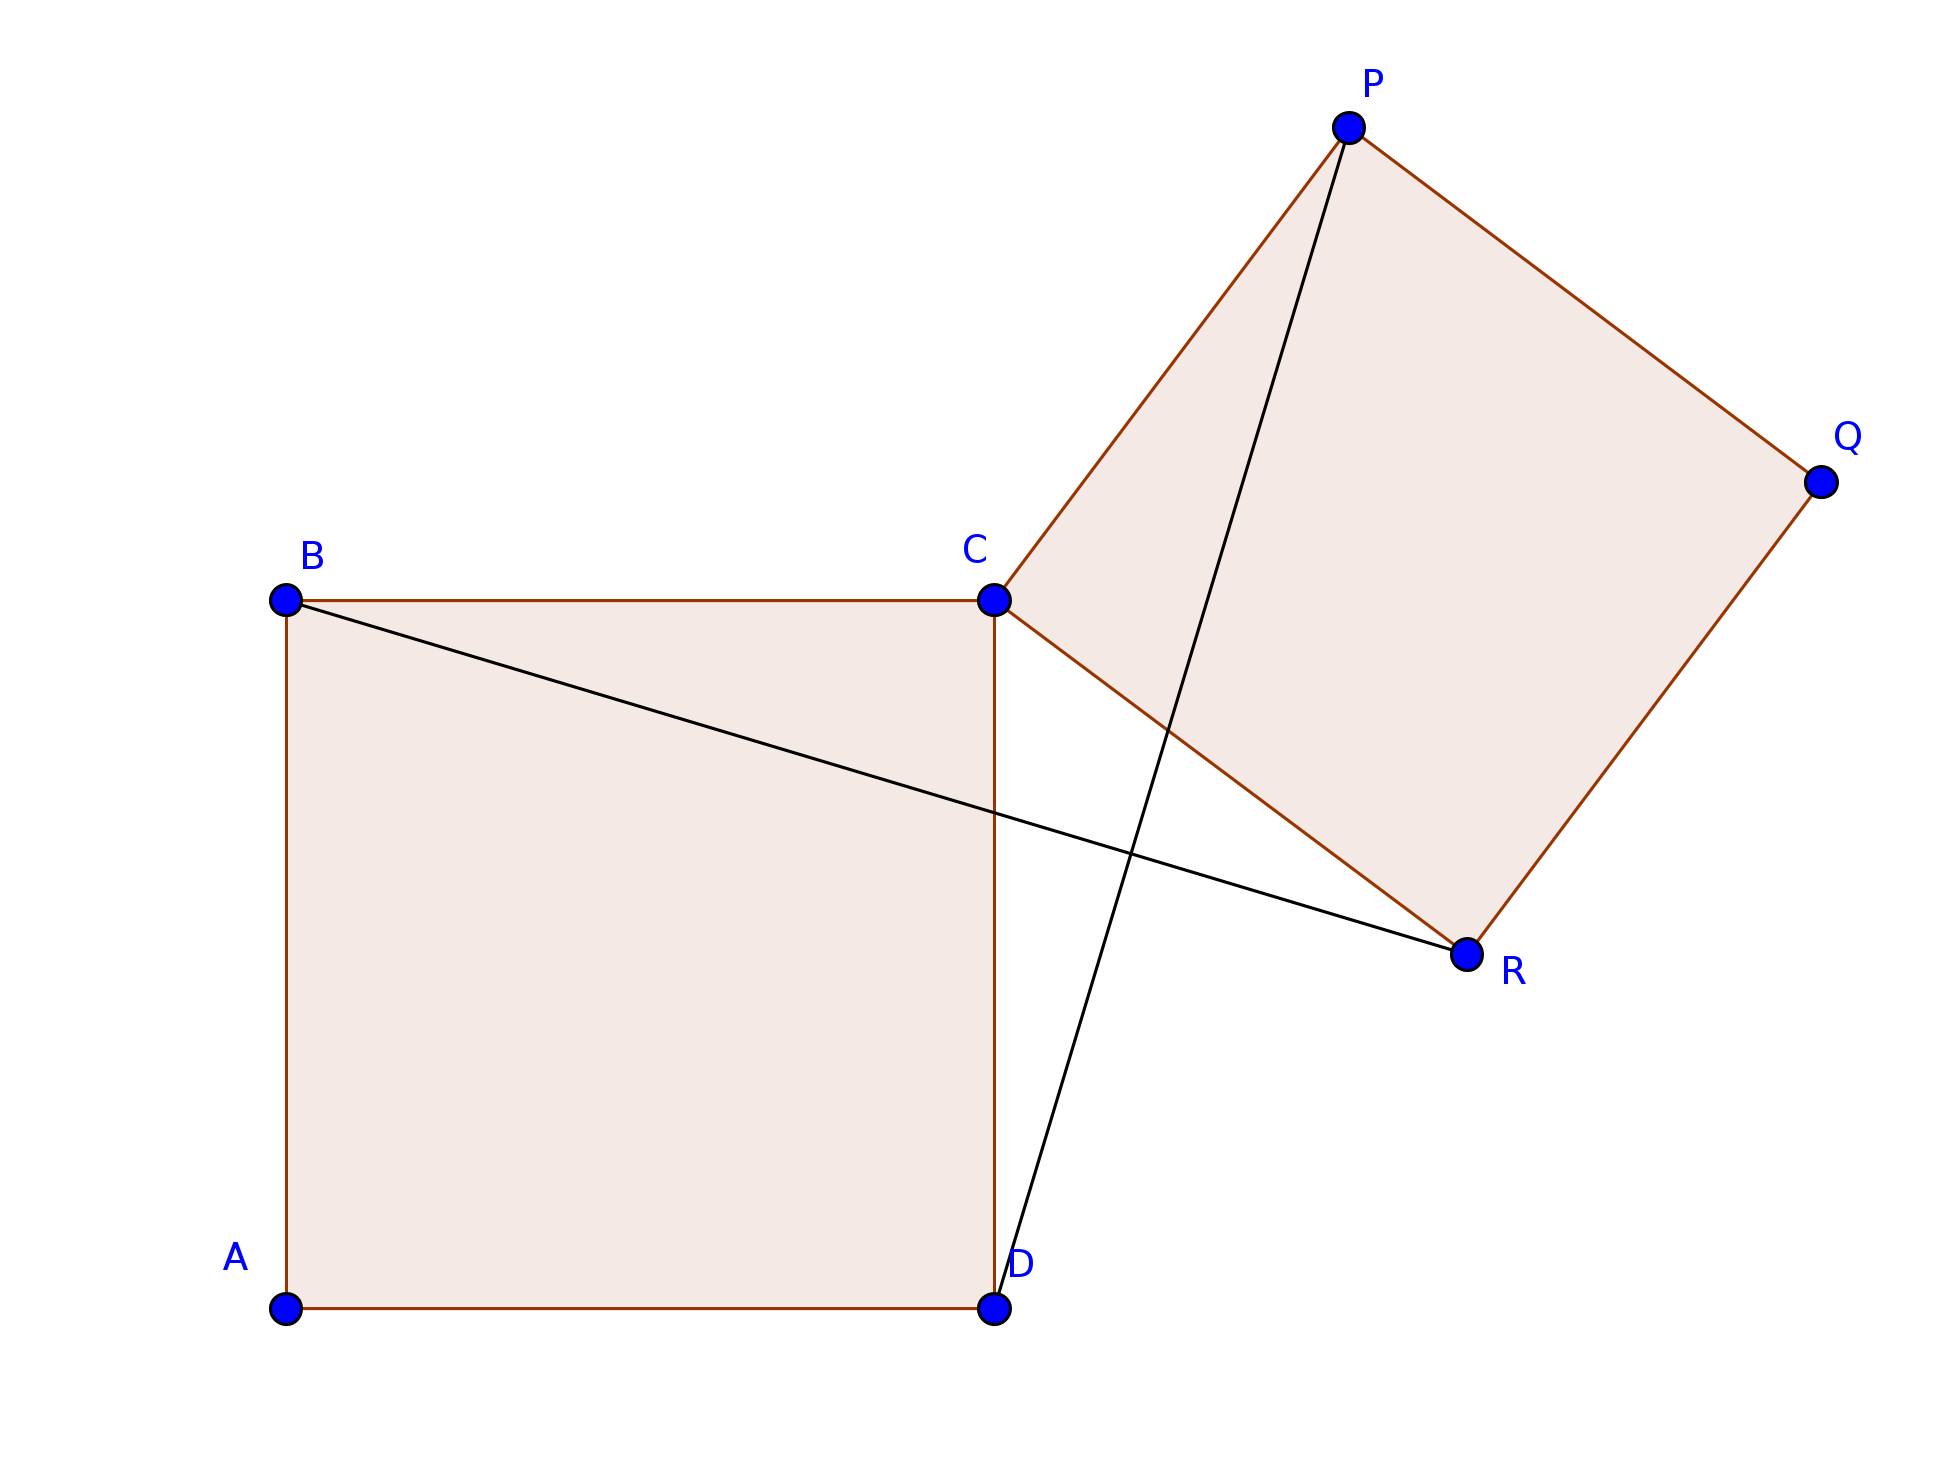
\includegraphics[width=.45\textwidth]{georazn01}
	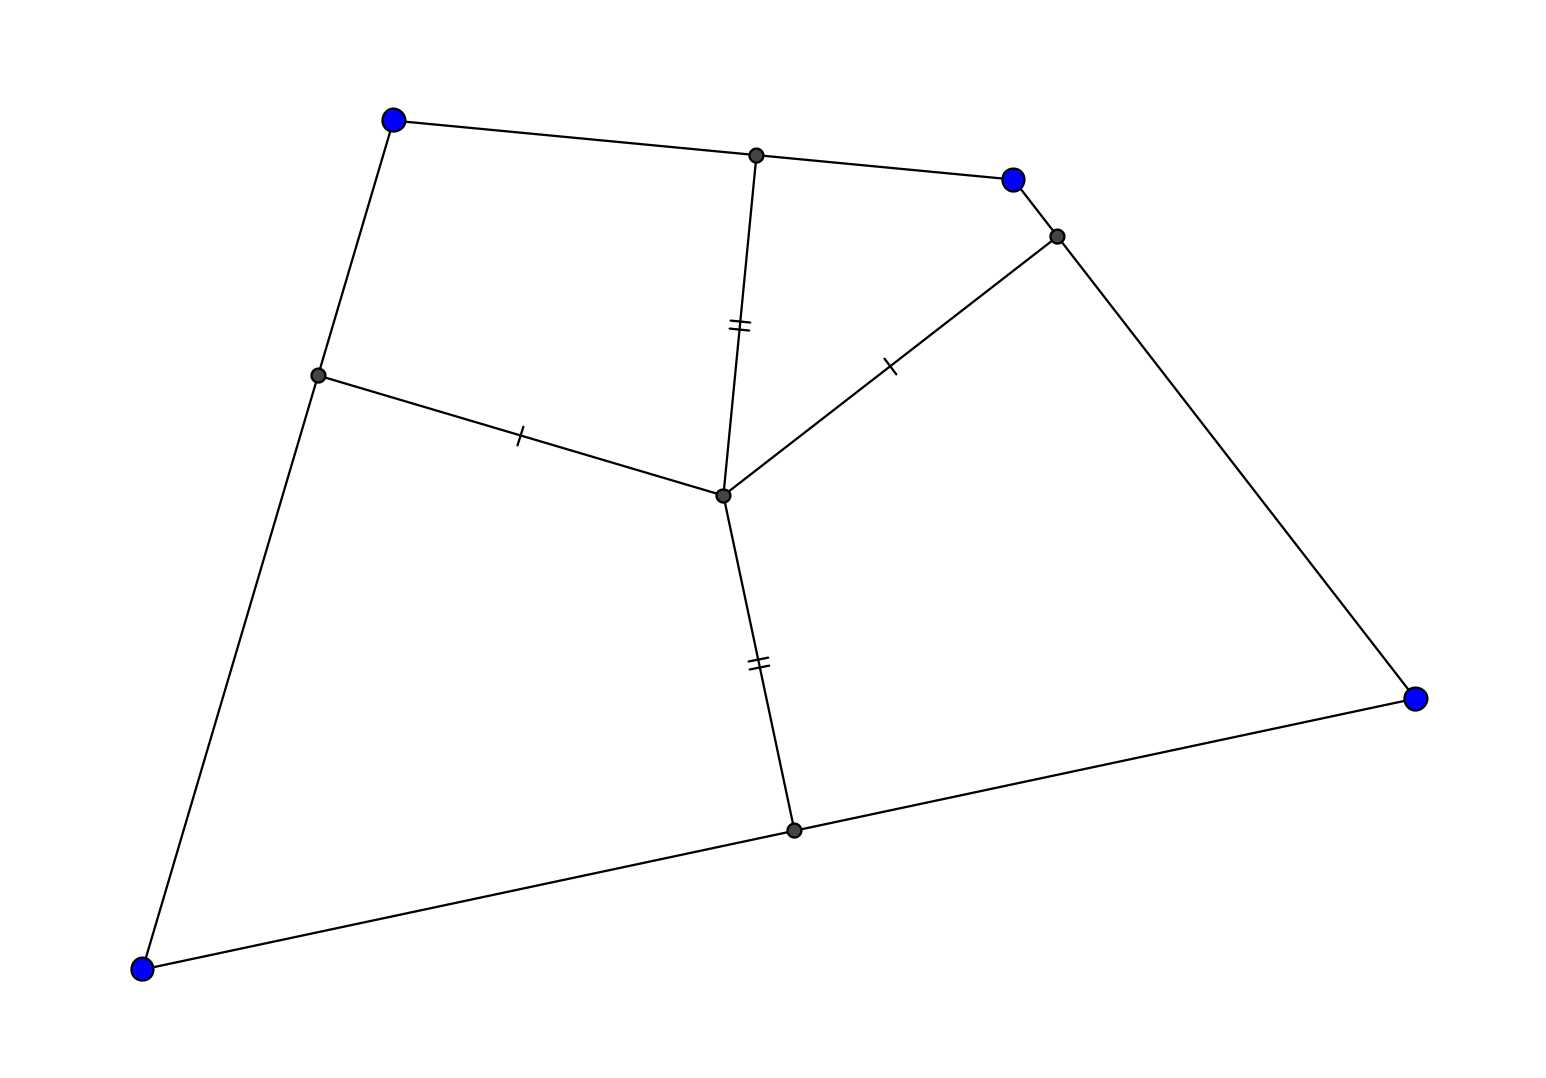
\includegraphics[width=.45\textwidth]{georazn02}
\end{center}

\item На стороне $BC$ квадрата $ABCD$ выбрана точка $M$. На стороне $CD$ выбрана такая точка $P$, что $AP\perp MD$. На стороне $AB$ выбрана такая точка $Q$, что $DQ\perp MA$. Докажите, что прямая $PQ$ проходит через центр квадрата.
%симметричная картинка

\item Бильярд имеет форму остроугольного треугольника $ABC$. Из точки $K$ стороны $AB$ выпустили бильярдный шар, который отразился (по правилу угол падения равен углу отражения) в точках $L, M$ от сторон $BC, CA$, возвратился в точку $K$ и вновь вышел на траекторию $KLM$. Докажите, что точки $K, L, M$~--- точки основания высот треугольника $ABC$.

\item Внутри острого угла $XOY$ взяты точки $M$ и $N$ так, что $\angle XON = \angle YOM$. На отрезке $OX$ выбирается точка $Q$ так, что $\angle NQO = \angle MQX$, а на отрезке $OY$ выбирается точка $P$ так, что $\angle NPO = \angle MPY$. Докажите, что длины ломаных $MPN$ и $MQN$ равны.

\item В треугольнике $ABC$ на сторонах $AC$ и $BC$ взяты точки $X$ и $Y$ такие, что $\angle ABX = \angle YAC$, $\angle AYB = \angle BXC$, $XC = YB$. Найдите углы треугольника $ABC$.
% 4 признак + небольшой счёт углов

\item На~сторонах $AB$ и~$AD$ квадрата $ABCD$ выбраны точки $N$ и~$P$ соответственно,
а~на~отрезке~$AN$ выбрана точка~$Q$ так, что $NP = NC$
и~$\angle QPN = \angle NCB$.
Докажите, что $\angle BCQ = \frac{1}{2} \angle AQP$.

%\item Даны два выпуклых многоугольника $A_1A_2A_3A_4...A_n$ и $B_1B_2B_3B_4...B_n$. Известно, что $A_1A_2 = B_1B_2$, $A_2A_3 = B_2B_3,..., A_nA_1 = B_nB_1$ и $n - 3$ угла одного многоугольника равны соответственным углам другого. Будут ли многоугольники равны?

\end{problems}
\resetproblem
\vspace{1cm}
\addcontentsline{toc}{abcd}{\bf Полуинвариант. 22 июля}
\begin{center}
\textbf{\Large Легенды о короле Артуре}\\
\textit{22.07.16}
\end{center}

\epigraph{\it Всё выше, выше и выше\\
Стремим мы полёт наших птиц,\\
И в каждом пропеллере дышит\\
Спокойствие наших границ.}{Марш авиаторов}

\textbf{Упражнение 1.}\\
На доске написано несколько натуральных чисел. Каждую минуту выбирают какие-то два из них ($x$ и $y$) и заменяют их на числа $x-2$ и $y+1$. Докажите, что рано или поздно на доске появится отрицательное число.\\
\textbf{Упражнение 2.}\\
По кругу стоит 101 мудрец. Каждый из них либо считает, что Земля вращается вокруг Юпитера, либо считает, что Юпитер вращается вокруг Земли. Один раз в минуту все мудрецы одновременно оглашают свои мнения. Сразу после этого каждый мудрец, оба соседа которого думают иначе, чем он, меняет своё мнение, а остальные – не меняют. Докажите, что через некоторое время мнения перестанут меняться.

\begin{problems}

\item При дворе у короля Артура собралась свита из верных рыцарей. Рыцари дружны, однако в любом коллективе есть разногласия. Известно также, что любой рыцарь имеет не более трех врагов.  Король Артур собирается в поход, карать мятежных южных баронов. Докажите, что Артур сможет собрать карательный отряд и оставить остальных рыцарей править городом так, чтобы у каждый имел не более одного врага в своей группе?
% ну все и так помнят


\item Мерлин предложил королю Артуру, уставшему от походов, поиграть вот в такую игру: есть прямоугольная таблице $ m \times n$,  в ней записаны какие-то действительные числа. Разрешается менять знак сразу у всех чисел какой-либо строки или столбца. Докажите, что такими операциями можно добиться того, чтобы в каждой строке и в каждом столбце сумма чисел была неотрицательна.

\item Король Артур устроил пир по поводу перемирия, на который пригласил южных мятежных баронов. У каждого южного мятежного барона есть придворный шут, который хочет спеть песенку. Известно, что каждая песенка оскорбительна не более чем для
трех других южных мятежных Баронств. Каждый барон, дослушав своего шута, тут же уезжает и не слышит песенки, прозвучавшие после него. Докажите, что мудрый Мерлин может расположить выступления шутов в таком порядке, что каждый барон услышит не более трех оскорбительных песенок.

%сумма чисел во всей таблице увеличивается

%\item Из-за постоянных вооруженных разногласий по поводу политики, проводимой королем Артуром, его верным рыцарям некогда следить за своими землями. Управляющий заявил Ланселоту, что скоро участок рыцаря придет в негодность, ведь что уже 9 клеток его 100-клеточного квадратного поля поросли бурьяном. Известно, что бурьян за месяц распространяется на те и только те участки, у каждого из которых не менее двух соседних участков уже поражены бурьяном (участки соседние, если они имеют общую сторону). Докажите, что управляющий ошибается, и поле никогда не зарастет полностью. 
% граница бурьяна не возрастает

\item Король Артур постепенно завоевывает все новые и новые территории. В n окрестных графствах власть принадлежит либо королю, либо Нзависимому Южному Союзу Графов. Мятежные графы в большинстве своем очень трусливы. Каждый день в одном из графств( назовем его А) может поменяться власть. Это может произойти в том случае, если в большинстве граничащих с А графств власть принадлежит не тому, кто правит в графстве А(т.е., например,  если графство А примкнуло к Независимому Союзу, а большинство соседей присягнули Королю Артуру, и наоборот). Докажите, что смены правительств не могут продолжаться бесконечно. 
% После смены партии в стране количество ее стран-соседей той же партии увеличивается

\item  После карательного похода рыцари собрались за круглым столом и делят свою добычу. Известно лишь, что изначально у каждого рыцаря четное количество монет. По команде Мерлина каждый передает половину своих монет сидящему справа. Если после этого у кого-нибудь оказалось нечётное количество монет, то добрый южный барон, который не хочет, чтобы его повесили, добавляет этому рыцарю еще одну монету. Это повторяется много раз.  Доказать, что настанет время, когда у всех рыцарей будет поровну монет.

% Суммарная разность межу соседними дугами уменьшается 
%\item Даны две последовательности: 2, 4, 8, 16, 14, 10, 2 и 3, 6, 12. В каждой из них каждое число получено из предыдущего по одному и тому же закону.\\
%а) Найдите этот закон.\\
%б) Найдите все натуральные числа, переходящие сами в себя (по этому закону).\\
%в) Докажите, что число $2^{1991}$ после нескольких переходов станет однозначным.
%Следующее число -  удвоенная сумма цифр предыдущего. б - "Неподвижное число" - 18. в - Число не длится на 9 - значит, уменьшается
\item Темница короля Артура - длинный-длинный подземный коридор с камерами только по одну сторону, занумерованными числами от минус бесконечности до плюс бесконечности. В камерах находятся 9 узников (в одной камере могут быть заключены несколько узников). Их тюремщики скучают, и поэтому каждый день каких-то двух узников, обитающих в соседних камерах (k-й и (k+1)-й), переселяют соответственно в (k–1)-ю и (k+2)-ю комнаты. Докажите, что через конечное число дней тюремщики не смогут продолжать свою игру.(Узников, заключенных в одной камере, не расселяют.)

%\item В королевстве Артура магический турнир. На огромном поле соревнуются $n$ магов, никакие трое из них не стоят на одной прямой.По команде маги пускают фаерболы  в $n$ бесконечно длинных прямых заграждений(каждый - в свое), никакие два из заграждений не параллельны. Докажите, что Мерлин может так разбить магов на пары "маг - заграждение", что никакие два фаербола не столкнутся(Фаерболы интеллектуальные, и летят по наименьшему из возможных расстояний)
% Длины перпендикуляров уменьшаются
% Число пар врагов-соседей уменьшается
\item Прогуливаясь однажды по городскому базару инкогнито, Мерли увидел маленьких мошенников, играющих с горожанами в наперстки. Желая проучить мальчишек, Мерлин предложил им одно пари. Пари заключается в следуюшем: берется колода карт. Мальчишки переворачивают часть карт рубашкой вниз. Разрешается вынуть из колоды пачку из нескольких подряд идущих карт, в которой верхняя и нижняя карты лежат рубашкой вниз (в частности, можно вынуть просто одну карту рубашкой вниз), перевернуть эту пачку как одно целое и вставить в то же место колоды. Мерлин переворачивает ту пачку, на которую укажут мальчики (перевернуть что-то нужно каждым ходом). Мерлин выигрывает, если в колоде все карты лягут рубашкой вверх. Докажите, что в конце концов Мерлин выиграет.
% Полуинвариант: если закодировать буквами - в -вверх и н — вниз, то каждая операция улучшает лексикографический порядок

\end{problems}
\resetproblem
\vspace{1cm}
\addcontentsline{toc}{abcd}{\bf Разнобой. 22 июля}
\begin{center}
\textbf{\Large Разнобой}\\
%\textit{Профи}\\
\textit{22.07.16}
\end{center}

\epigraph{\it Дорогие друзья! Пришло время прощаться. Спасибо всем, кто пришёл сюда в этот зимний снежный день! Мы вас любим.}{С. Калугин}

\begin{problems}
\item На некоторых белых клетках шахматной доски стоят короли. Докажите, что их можно покрасить в два цвета так, чтобы короли одинакового цвета друг друга не били.

\item Выписаны 1000 целых чисел. Докажите, что их можно покрасить в два цвета так, чтобы отношение чисел одинакового цвета не было простым числом. 

\item В классе 30 учеников, у каждого ровно по 2 друга. Докажите, что можно организовать не менее 10 дежурств так, чтобы дежурили по двое друзей, и никто не дежурил дважды. Всегда ли можно организовать 11 дежурств?

\item Шах разбил свой квадратный одноэтажный дворец на 64 одинаковые квадратные комнаты, разделил комнаты на семь квартир (проделав двери в некоторых перегородках между комнатами) и в каждой квартире поселил по жене. Жены могут ходить по всем комнатам своей квартиры, не заходя к другим. Какое наименьшее число дверей пришлось проделать во внутренних стенах?

\item Назовем крокодилом шахматную фигуру, ход которой заключается в прыжке на $m$ клеток по вертикали или по горизонтали и затем на $n$ клеток в перпендикулярном направлении. Докажите, что для любых $m$ и $n$ можно так раскрасить клетчатую доску $1000000\times 1000000$ в два цвета (для каждых конкретных $m$ и $n$ своя раскраска), что любые две клетки, соединенные одним ходом крокодила, будут покрашены в разные цвета.

%\item Петя поставил на доску $50 \times 50$ несколько фишек, в каждую клетку~--- не больше одной. Докажите, что у Васи есть способ поставить на свободные поля этой же доски не более 99 новых фишек (возможно, ни одной) так, чтобы по-прежнему в каждой клетке стояло не больше одной фишки, и в каждой строке и каждом столбце этой доски оказалось чётное количество фишек.
%В норке живёт семья из 24 мышей. Каждую ночь ровно четыре из них отправляются на склад за сыром. Может ли так получиться, что в некоторый момент времени каждая мышка побывала на складе с каждой ровно по одному разу?
%Дана ладья, которой разрешается делать ходы только длиной в одну клетку. Доказать, что она может обойти все клетки прямоугольной шахматной доски, побывав на каждой клетке ровно один раз, и вернуться в начальную клетку тогда и только тогда, когда число клеток на доске чётно.

%Дано натуральное число  $n \geq 2$.  Рассмотрим все такие покраски клеток доски n×n в $k$ цветов, что каждая клетка покрашена ровно в один цвет и все $k$ цветов встречаются. При каком наименьшем $k$ в любой такой покраске найдутся четыре окрашенных в четыре разных цвета клетки, расположенные в пересечении двух строк и двух столбцов?
%\item Каждая деталь конструктора <<Юный паяльщик>>~--- это скобка в виде буквы П, состоящая из трёх единичных отрезков. Можно ли из деталей этого конструктора спаять полный проволочный каркас куба $2\times2\times2$, разбитого на кубики $1\times1\times1$? (Каркас состоит из 27 точек, соединенных единичными отрезками; любые две соседние точки должны быть соединены ровно одним проволочным отрезком.)
\end{problems}

\resetproblem
\vspace{1cm}

\end{document}